\documentclass[8pt,aspectratio=169]{beamer}
%\documentclass[8pt,aspectratio=169,handout]{beamer}

% Beamer theme
% Install from https://github.com/jolars/moloch or https://ctan.org/pkg/moloch
\usetheme{moloch}

% Packages
\usepackage{biblatex}
\usepackage{booktabs}
\usepackage{fontawesome}
\usepackage{graphicx}
\usepackage{hyperref}
\usepackage{tikz}

% Bibtex file
\ExecuteBibliographyOptions{doi=false,eprint=false,isbn=false,url=false}
\addbibresource{biblio.bib}


% Tikz libraries
\usetikzlibrary{arrows.meta, positioning}

% hyperref settings
% (color definition: https://latexcolor.com)
\definecolor{pastelred}{rgb}{1.0, 0.41, 0.38}
\definecolor{steelblue}{rgb}{0.27, 0.51, 0.71}
\hypersetup{
  colorlinks=true,
  linkcolor=steelblue,
  urlcolor=steelblue,
  citecolor=steelblue
}

% import urls
\newcommand{\githubURL}{%
  https://github.com/jpasquier/pres-simpson%
}
\newcommand{\jmorrisBlogpostURL}{%
  https://www.covid-datascience.com/post/israeli-data-how-can-efficacy-vs-severe-disease-be-strong-when-60-of-hospitalized-are-vaccinated%
}
\newcommand{\imhDashboardURL}{%
  https://datadashboard.health.gov.il/COVID-19/general%
}
\newcommand{\whoVaxEfficayURL}{%
  https://www.who.int/news-room/feature-stories/detail/vaccine-efficacy-effectiveness-and-protection%
}
\newcommand{\charigURL}{%
  https://doi.org/10.1136/bmj.292.6524.879%
}


% Commands
\newcommand{\bs}{\vspace{\baselineskip}}
\newcommand{\Vax}{\text{Vax}}
\newcommand{\Unvax}{\text{Unvax}}
\newcommand{\Severe}{\text{Severe}}
\newcommand{\Effectiveness}{\text{Effectiveness}}
\newcommand{\Prob}{\text{Prob}}
\newcommand{\logit}{\text{logit}}

% ─────────────────────────────────────────────────────────────────────────────

% Title page
\title{Simpson's Paradox}
\author{Jérôme Pasquier}
\date{October 24, 2024}

% ─────────────────────────────────────────────────────────────────────────────

\begin{document}

% ─────────────────────────────────────────────────────────────────────────────

\maketitle

% ─────────────────────────────────────────────────────────────────────────────

\begin{frame}

  \centering

  \faGithub \hspace{1pt} \href{\githubURL}{\githubURL}

\end{frame}

% ─────────────────────────────────────────────────────────────────────────────

\begin{frame}{Professional Experience and Education}

  \textbf{Current Position:}
  \begin{itemize}
    \item {\bfseries Biostatistician, CSL Behring (2023–Present)} \\
      Expertise in pre-clinical research applications, including study design,
      drug candidate selection, and assay development.
  \end{itemize}

  \textbf{Previous Positions:}
  \begin{itemize}
    \item {\bfseries Biostatistician, Unisanté, University of Lausanne
      (2015–2023)} \\
      Supported statistical aspects of research, including writing protocols,
      performing analyses, and publishing articles.
    \item {\bfseries Scientific Collaborator, Federal Statistical Office
      (2013–2015, 2009–2012)} \\
      Focused on survey design, data analysis, and quality control for national
      projects.
    \item {\bfseries Teaching Assistant, University of Fribourg (2003–2008)} \\
      Assisted in mathematics instruction and interdisciplinary research.
  \end{itemize}

  \textbf{Education:}
  \begin{itemize}
    \item PhD in Mathematics, University of Fribourg (2003–2008) \\
      Thesis: Stochastic models for gene regulation.
  \end{itemize}

\end{frame}

% ─────────────────────────────────────────────────────────────────────────────

\begin{frame}{Covid-19 Pfizer Vaccine Effectiveness in Israel in 2021}

  \begin{center}

    \begin{minipage}{.75\textwidth}

       
\includegraphics[width=.35\textwidth]{%
         images/becker_hospital_review_header.png}

       \centering

       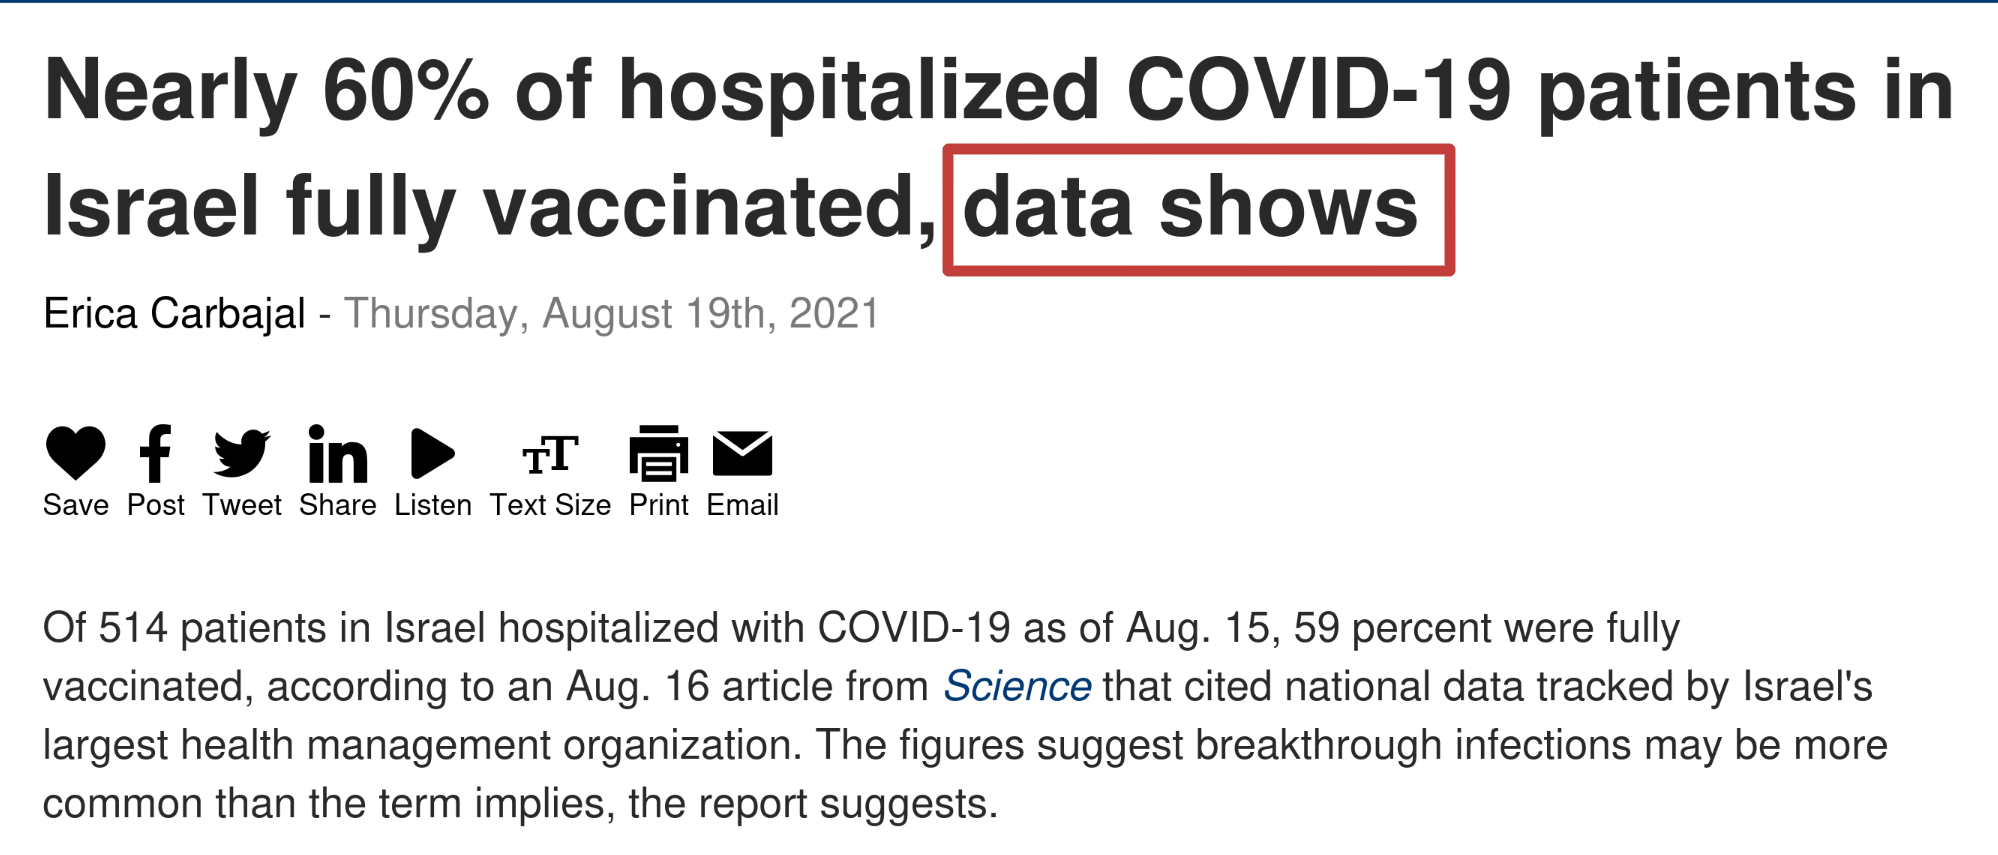
\includegraphics[width=\textwidth]{%
         images/becker_hospital_review_article_1.png}

       \noindent\rule{\textwidth}{0.4pt}

       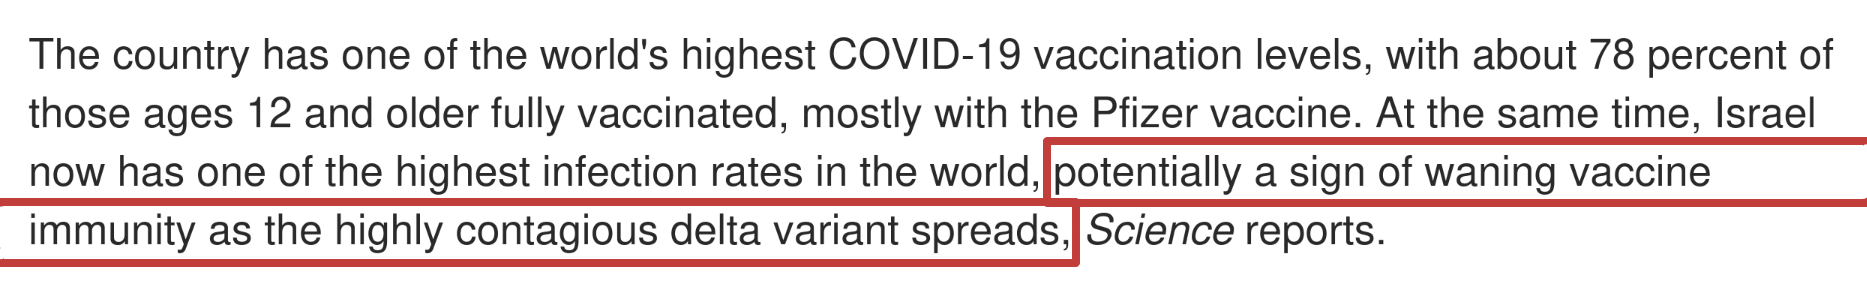
\includegraphics[width=\textwidth]{%
         images/becker_hospital_review_article_2.png}

    \end{minipage}

  \end{center}

\end{frame}

% ─────────────────────────────────────────────────────────────────────────────

\begin{frame}{What Do the Data Show?}

  Indeed, data show that approximately 60\% of patients with severe COVID-19
  infection were fully vaccinated.

  \bs

  % +-------------+-------------+------------+
  % |severe cases |severe unvax |severe vax  |
  % +-------------+-------------+------------+
  % |515          |214 (41.6%)  |301 (58.4%) |
  % +-------------+-------------+------------+

  % latex table generated in R 4.4.1 by xtable 1.8-4 package
% Wed Oct 23 19:34:50 2024
\begin{table}[ht]
\centering
\begin{tabular}{lll}
  \toprule
{\textbf{severe cases}} & {\textbf{severe unvax}} & {\textbf{severe vax}} \\ 
  \midrule
515 & 214 (41.6\%) & 301 (58.4\%) \\ 
   \bottomrule
\end{tabular}
\end{table}


  \bs

  Data were downloaded from the \href{\imhDashboardURL}{Israeli Ministry of
  Health Dashboard} on August 15, 2021, by Jeffrey Morris and can be found in a
  \href{\jmorrisBlogpostURL}{blog post} by him.

\end{frame}

% ─────────────────────────────────────────────────────────────────────────────

\begin{frame}{Israeli Data}

  % +------ +------------+------------+--------+--------+---------------+
  % | age   | population | population | severe | severe | effectiveness |
  % | group | unvax      | vax        | unvax  | vax    |               |
  % +-------+------------+------------+--------+--------+---------------+
  % | All   | 1302912    | 5634634    | 214    | 301    | 67.5%         |
  % | (≥12) | (18.8%)    | (81.2%)    | (16.4) | (5.3)  |               |
  % +------ +------------+------------+--------+--------+---------------+

  % latex table generated in R 4.4.1 by xtable 1.8-4 package
% Wed Oct 23 19:34:50 2024
\begin{table}[ht]
\centering
\begin{tabular}{lrrrrr}
  \toprule
  & \multicolumn{2}{c}{\textbf{Population (\%)}} & \multicolumn{2}{c}{\textbf{Severe Cases (per 100k\footnotemark{})}} & \\
 \cmidrule(lr){2-3} \cmidrule(lr){4-5}
 \textbf{Age Group} & \textbf{Unvax} & \textbf{Vax} & \textbf{Unvax} & \textbf{Vax} & \textbf{Effectiveness} \\
 \midrule
All ($\geq$12) & 1302912 (18.8\%) & 5634634 (81.2\%) & 214 (16.4) & 301 (5.3) & 67.5\% \\ 
   \bottomrule
\end{tabular}
\end{table}


  \footnotetext{
    \( \text{severe\_(un)vax\_per\_100k} =
    \cfrac{\text{severe\_(un)vax}}{\text{population\_(un)vax}} \times 10^5 \).
  }

  \bs

  The effectiveness of the vaccine is defined as the reduction in infection
  rate\footnotemark{}.

  \footnotetext{
    See \href{\whoVaxEfficayURL}{World Health Organization website}.
  }

  \bs

  If a vaccine has an effectiveness of 80 percent:

  \begin{itemize}

    \item It does not mean that the vaccine will only work 80\% of the time.

    \item It means that in a vaccinated population, there will be 80\% fewer
      people infected.

  \end{itemize}

  \[
    \Prob(\Severe \mid \Vax)
    = (1 - \Effectiveness) \times \Prob(\Severe \mid \Unvax)
  \]

  \[
    \Effectiveness
    = 1 - \frac{\Prob(\Severe \mid \Vax)}{\Prob(\Severe \mid \Unvax)}
    \qquad \textbf{Here:} \quad
    \Effectiveness = 1 - \frac{5.3}{16.4} = 67.5\%
  \]

\end{frame}

% ─────────────────────────────────────────────────────────────────────────────

\begin{frame}{Let's Break Down the Data by Age Group}

  % +-------+------------+------------+--------+--------+---------------+
  % | age   | population | population | severe | severe | effectiveness |
  % | group | unvax      | vax        | unvax  | vax    |               |
  % +-------+------------+------------+--------+--------+---------------+
  % | All   | 1302912    | 5634634    | 214    | 301    | 67.5%         |
  % | (≥12) | (18.8%)    | (81.2%)    | (16.4) | (5.3)  |               |
  % +-------+------------+------------+--------+--------+---------------+
  % | <50   | 1116834    | 3501118    | 43     | 11     | 91.8%         |
  % |       | (24.2%)    | (75.8%)    | (3.9)  | (0.3)  |               |
  % +-------+------------+------------+--------+--------+---------------+
  % | ≥50   | 186078     | 2133516    | 171    | 290    | 85.2%         |
  % |       | (8%)       | (92%)      | (91.9) | (13.6) |               |
  % +-------+------------+------------+--------+--------+---------------+

  \begin{overprint}

    \onslide<1>

    % latex table generated in R 4.4.1 by xtable 1.8-4 package
% Wed Oct 23 19:34:51 2024
\begin{table}[ht]
\centering
\begin{tabular}{lrrrrr}
  \toprule
  & \multicolumn{2}{c}{\textbf{Population (\%)}} & \multicolumn{2}{c}{\textbf{Severe Cases (per 100k)}} & \\
 \cmidrule(lr){2-3} \cmidrule(lr){4-5}
 \textbf{Age Group} & \textbf{Unvax} & \textbf{Vax} & \textbf{Unvax} & \textbf{Vax} & \textbf{Effectiveness} \\
 \midrule
All ($\geq$12) & 1302912 (18.8\%) & 5634634 (81.2\%) & 214 (16.4) & 301 (5.3) & 67.5\% \\
  <50 & 1116834 (24.2\%) & 3501118 (75.8\%) & 43 (3.9) & 11 (0.3) & 91.8\% \\
  $\geq$50 &  &  &  &  &  \\
   \bottomrule
\end{tabular}
\end{table}


    \onslide<2->

    % latex table generated in R 4.4.1 by xtable 1.8-4 package
% Wed Oct 23 19:34:51 2024
\begin{table}[ht]
\centering
\begin{tabular}{lrrrrr}
  \toprule
  & \multicolumn{2}{c}{\textbf{Population (\%)}} & \multicolumn{2}{c}{\textbf{Severe Cases (per 100k)}} & \\
 \cmidrule(lr){2-3} \cmidrule(lr){4-5}
 \textbf{Age Group} & \textbf{Unvax} & \textbf{Vax} & \textbf{Unvax} & \textbf{Vax} & \textbf{Effectiveness} \\
 \midrule
All ($\geq$12) & 1302912 (18.8\%) & 5634634 (81.2\%) & 214 (16.4) & 301 (5.3) & 67.5\% \\ 
  <50 & 1116834 (24.2\%) & 3501118 (75.8\%) & 43 (3.9) & 11 (0.3) & 91.8\% \\ 
  $\geq$50 & 186078 (8\%) & 2133516 (92\%) & 171 (91.9) & 290 (13.6) & 85.2\% \\ 
   \bottomrule
\end{tabular}
\end{table}


  \end{overprint}

  \bs

  \begin{overprint}

    \onslide<1>

    We have good effectiveness in the <50 age group!

    \bs

    So, I guess that the effectiveness is very low in the $\ge$50 age group.

    \onslide<2>

    \bs

    \begin{center}

      \Huge{\bfseries WTF?}

    \end{center}


    \onslide<3->

    The effectiveness measured in the whole population is lower than the
    effectiveness measured in each age group.

    \bs

    It seems paradoxical. Why do we have an effectiveness lower than
    70\% in the whole population while we have an effectiveness higher than
    85\% in each age group?

    \bs

    This paradoxical effect is what we call {\bfseries \large Simpson's
    Paradox}.

  \end{overprint}

\end{frame}

% ─────────────────────────────────────────────────────────────────────────────

\begin{frame}{Let's Break Down the Data by Age Group}

  % +-------+------------+------------+---------+--------+---------------+
  % | age   | population | population | severe  | severe | effectiveness |
  % | group | unvax      | vax        | unvax   | vax    |               |
  % +-------+------------+------------+---------+--------+---------------+
  % | 12-15 | 383649     | 184549     | 1       | 0      | 100%          |
  % |       | (67.5%)    | (32.5%)    | (0.3)   | (0)    |               |
  % +-------+------------+------------+---------+--------+---------------+
  % | 16-19 | 127745     | 429109     | 2       | 0      | 100%          |
  % |       | (22.9%)    | (77.1%)    | (1.6)   | (0)    |               |
  % +-------+------------+------------+---------+--------+---------------+
  % | 20-29 | 265871     | 991408     | 4       | 0      | 100%          |
  % |       | (21.1%)    | (78.9%)    | (1.5)   | (0)    |               |
  % +-------+------------+------------+---------+--------+---------------+
  % | 30-39 | 194213     | 968837     | 12      | 2      | 96.7%         |
  % |       | (16.7%)    | (83.3%)    | (6.2)   | (0.2)  |               |
  % +-------+------------+------------+---------+--------+---------------+
  % | 40-49 | 145355     | 927214     | 24      | 9      | 94.1%         |
  % |       | (13.6%)    | (86.4%)    | (16.5)  | (1)    |               |
  % +-------+------------+------------+---------+--------+---------------+
  % | 50-59 | 84545      | 747949     | 34      | 22     | 92.7%         |
  % |       | (10.2%)    | (89.8%)    | (40.2)  | (2.9)  |               |
  % +-------+------------+------------+------- -+--------+---------------+
  % | 60-69 | 65205      | 665717     | 50      | 58     | 88.6%         |
  % |       | (8.9%)     | (91.1%)    | (76.7)  | (8.7)  |               |
  % +-------+------------+------------+---------+--------+---------------+
  % | 70-79 | 20512      | 464336     | 39      | 92     | 89.6%         |
  % |       | (4.2%)     | (95.8%)    | (190.1) | (19.8) |               |
  % +-------+------------+------------+---------+--------+---------------+
  % | 80-89 | 12683      | 208911     | 32      | 100    | 81%           |
  % |       | (5.7%)     | (94.3%)    | (252.3) | (47.9) |               |
  % +-------+------------+------------+---------+--------+---------------+
  % | 90+   | 3132       | 46602      | 16      | 18     | 92.4%         |
  % |       | (6.3%)     | (93.7%)    | (510.8) | (38.6) |               |
  % +-------+------------+------------+---------+--------+---------------+

  % latex table generated in R 4.4.1 by xtable 1.8-4 package
% Wed Oct 23 19:34:51 2024
\begin{table}[ht]
\centering
\begin{tabular}{lrrrrr}
  \toprule
  & \multicolumn{2}{c}{\textbf{Population (\%)}} & \multicolumn{2}{c}{\textbf{Severe Cases (per 100k)}} & \\
 \cmidrule(lr){2-3} \cmidrule(lr){4-5}
 \textbf{Age Group} & \textbf{Unvax} & \textbf{Vax} & \textbf{Unvax} & \textbf{Vax} & \textbf{Effectiveness} \\
 \midrule
12-15 & 383649 (67.5\%) & 184549 (32.5\%) & 1 (0.3) & 0 (0) & 100\% \\ 
  16-19 & 127745 (22.9\%) & 429109 (77.1\%) & 2 (1.6) & 0 (0) & 100\% \\ 
  20-29 & 265871 (21.1\%) & 991408 (78.9\%) & 4 (1.5) & 0 (0) & 100\% \\ 
  30-39 & 194213 (16.7\%) & 968837 (83.3\%) & 12 (6.2) & 2 (0.2) & 96.7\% \\ 
  40-49 & 145355 (13.6\%) & 927214 (86.4\%) & 24 (16.5) & 9 (1) & 94.1\% \\ 
  50-59 & 84545 (10.2\%) & 747949 (89.8\%) & 34 (40.2) & 22 (2.9) & 92.7\% \\ 
  60-69 & 65205 (8.9\%) & 665717 (91.1\%) & 50 (76.7) & 58 (8.7) & 88.6\% \\ 
  70-79 & 20512 (4.2\%) & 464336 (95.8\%) & 39 (190.1) & 92 (19.8) & 89.6\% \\ 
  80-89 & 12683 (5.7\%) & 208911 (94.3\%) & 32 (252.3) & 100 (47.9) & 81\% \\ 
  90+ & 3132 (6.3\%) & 46602 (93.7\%) & 16 (510.8) & 18 (38.6) & 92.4\% \\ 
   \bottomrule
\end{tabular}
\end{table}


\end{frame}

% ─────────────────────────────────────────────────────────────────────────────

\begin{frame}{So What's the Problem?}

  \begin{center}

    \onslide<2>{{\bfseries \Large Confounding}}

    \bs

    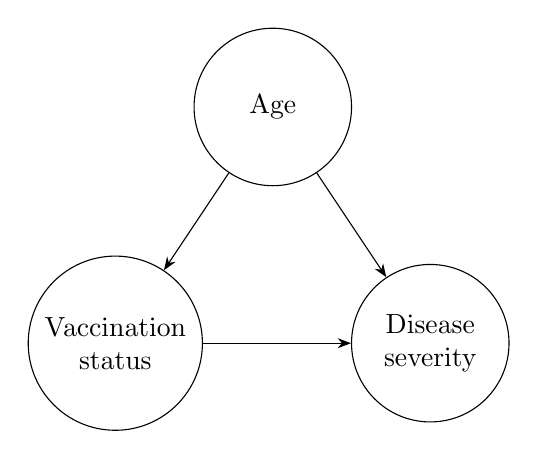
\begin{tikzpicture}[>=Stealth]

      % Set common node style
      \tikzset{
        mynode/.style={draw, circle, minimum size=2cm, align=center},
      }

      % Nodes
      \node (exposure) [mynode] at (0,0) {Vaccination\\status};
      \node (outcome) [mynode] at (4,0) {Disease\\severity};

      \onslide<2->{
        \node (confounder) [mynode] at (2,3) {Age};
      }

      % Arrows
      \draw[->] (exposure) -- (outcome);

      \onslide<2->{
        \draw[->] (confounder) -- (exposure);
        \draw[->] (confounder) -- (outcome);
      }

    \end{tikzpicture}

  \end{center}

\end{frame}

% ─────────────────────────────────────────────────────────────────────────────

\begin{frame}{Unbalanced Data}

  The proportion of vaccinated people in each age group is different.

  \begin{table}[ht]
    \centering
    \begin{tabular}{lr}
      \toprule
      \textbf{Age Group} & \textbf{Vaccinated (\%)} \\
      \midrule
      <50                & 75.8\%                   \\
      $\ge$50            & 92.0\%                   \\
      \bottomrule
    \end{tabular}
  \end{table}

  \begin{figure}[!h]
    \centering
    \resizebox{.9\columnwidth}{!}{% Created by tikzDevice version 0.12.6 on 2024-10-23 19:34:51
% !TEX encoding = UTF-8 Unicode
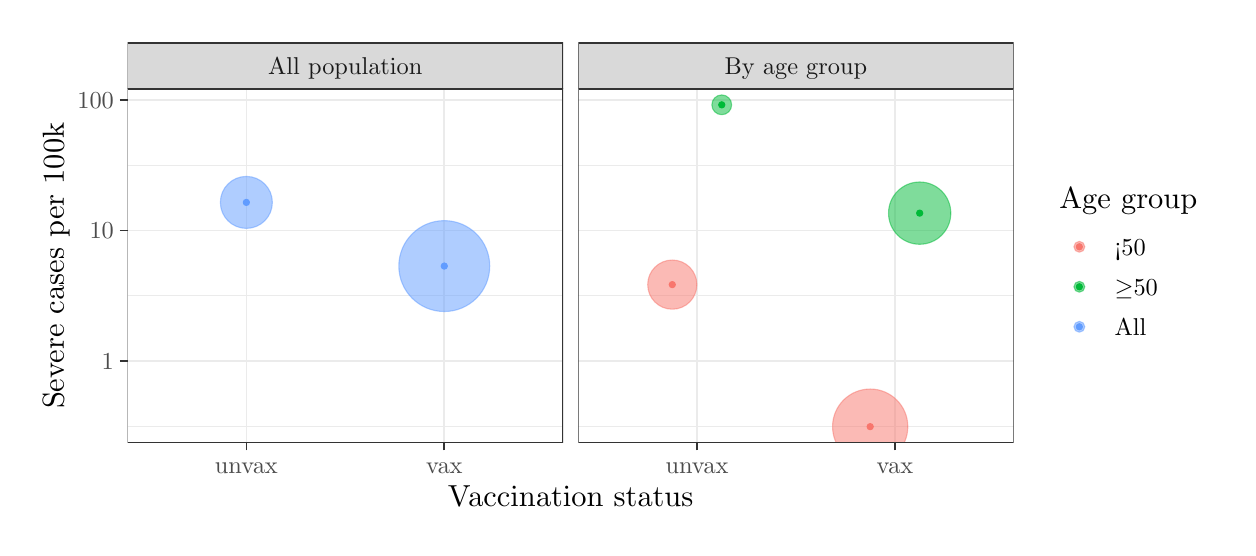
\begin{tikzpicture}[x=1pt,y=1pt]
\definecolor{fillColor}{RGB}{255,255,255}
\path[use as bounding box,fill=fillColor,fill opacity=0.00] (0,0) rectangle (433.62,180.67);
\begin{scope}
\path[clip] (  0.00,  0.00) rectangle (433.62,180.67);
\definecolor{drawColor}{RGB}{255,255,255}
\definecolor{fillColor}{RGB}{255,255,255}

\path[draw=drawColor,line width= 0.6pt,line join=round,line cap=round,fill=fillColor] (  0.00,  0.00) rectangle (433.62,180.68);
\end{scope}
\begin{scope}
\path[clip] ( 36.11, 30.69) rectangle (193.45,158.60);
\definecolor{fillColor}{RGB}{255,255,255}

\path[fill=fillColor] ( 36.11, 30.69) rectangle (193.45,158.60);
\definecolor{drawColor}{gray}{0.92}

\path[draw=drawColor,line width= 0.3pt,line join=round] ( 36.11, 36.63) --
	(193.45, 36.63);

\path[draw=drawColor,line width= 0.3pt,line join=round] ( 36.11, 83.79) --
	(193.45, 83.79);

\path[draw=drawColor,line width= 0.3pt,line join=round] ( 36.11,130.94) --
	(193.45,130.94);

\path[draw=drawColor,line width= 0.6pt,line join=round] ( 36.11, 60.21) --
	(193.45, 60.21);

\path[draw=drawColor,line width= 0.6pt,line join=round] ( 36.11,107.36) --
	(193.45,107.36);

\path[draw=drawColor,line width= 0.6pt,line join=round] ( 36.11,154.52) --
	(193.45,154.52);

\path[draw=drawColor,line width= 0.6pt,line join=round] ( 79.02, 30.69) --
	( 79.02,158.60);

\path[draw=drawColor,line width= 0.6pt,line join=round] (150.54, 30.69) --
	(150.54,158.60);
\definecolor{drawColor}{RGB}{97,156,255}
\definecolor{fillColor}{RGB}{97,156,255}

\path[draw=drawColor,draw opacity=0.50,line width= 0.4pt,line join=round,line cap=round,fill=fillColor,fill opacity=0.50] ( 79.02,117.53) circle (  9.39);

\path[draw=drawColor,draw opacity=0.50,line width= 0.4pt,line join=round,line cap=round,fill=fillColor,fill opacity=0.50] (150.54, 94.52) circle ( 16.42);
\definecolor{drawColor}{RGB}{97,156,255}
\definecolor{fillColor}{RGB}{97,156,255}

\path[draw=drawColor,line width= 0.4pt,line join=round,line cap=round,fill=fillColor] ( 79.02,117.53) circle (  1.11);

\path[draw=drawColor,line width= 0.4pt,line join=round,line cap=round,fill=fillColor] (150.54, 94.52) circle (  1.11);
\definecolor{drawColor}{gray}{0.20}

\path[draw=drawColor,line width= 0.6pt,line join=round,line cap=round] ( 36.11, 30.69) rectangle (193.45,158.60);
\end{scope}
\begin{scope}
\path[clip] (198.95, 30.69) rectangle (356.30,158.60);
\definecolor{fillColor}{RGB}{255,255,255}

\path[fill=fillColor] (198.95, 30.69) rectangle (356.30,158.60);
\definecolor{drawColor}{gray}{0.92}

\path[draw=drawColor,line width= 0.3pt,line join=round] (198.95, 36.63) --
	(356.30, 36.63);

\path[draw=drawColor,line width= 0.3pt,line join=round] (198.95, 83.79) --
	(356.30, 83.79);

\path[draw=drawColor,line width= 0.3pt,line join=round] (198.95,130.94) --
	(356.30,130.94);

\path[draw=drawColor,line width= 0.6pt,line join=round] (198.95, 60.21) --
	(356.30, 60.21);

\path[draw=drawColor,line width= 0.6pt,line join=round] (198.95,107.36) --
	(356.30,107.36);

\path[draw=drawColor,line width= 0.6pt,line join=round] (198.95,154.52) --
	(356.30,154.52);

\path[draw=drawColor,line width= 0.6pt,line join=round] (241.87, 30.69) --
	(241.87,158.60);

\path[draw=drawColor,line width= 0.6pt,line join=round] (313.38, 30.69) --
	(313.38,158.60);
\definecolor{drawColor}{RGB}{248,118,109}
\definecolor{fillColor}{RGB}{248,118,109}

\path[draw=drawColor,draw opacity=0.50,line width= 0.4pt,line join=round,line cap=round,fill=fillColor,fill opacity=0.50] (232.93, 87.82) circle (  8.88);

\path[draw=drawColor,draw opacity=0.50,line width= 0.4pt,line join=round,line cap=round,fill=fillColor,fill opacity=0.50] (304.44, 36.50) circle ( 13.59);
\definecolor{drawColor}{RGB}{0,186,56}
\definecolor{fillColor}{RGB}{0,186,56}

\path[draw=drawColor,draw opacity=0.50,line width= 0.4pt,line join=round,line cap=round,fill=fillColor,fill opacity=0.50] (250.80,152.79) circle (  3.57);

\path[draw=drawColor,draw opacity=0.50,line width= 0.4pt,line join=round,line cap=round,fill=fillColor,fill opacity=0.50] (322.32,113.65) circle ( 11.25);
\definecolor{drawColor}{RGB}{248,118,109}
\definecolor{fillColor}{RGB}{248,118,109}

\path[draw=drawColor,line width= 0.4pt,line join=round,line cap=round,fill=fillColor] (232.93, 87.82) circle (  1.11);

\path[draw=drawColor,line width= 0.4pt,line join=round,line cap=round,fill=fillColor] (304.44, 36.50) circle (  1.11);
\definecolor{drawColor}{RGB}{0,186,56}
\definecolor{fillColor}{RGB}{0,186,56}

\path[draw=drawColor,line width= 0.4pt,line join=round,line cap=round,fill=fillColor] (250.80,152.79) circle (  1.11);

\path[draw=drawColor,line width= 0.4pt,line join=round,line cap=round,fill=fillColor] (322.32,113.65) circle (  1.11);
\definecolor{drawColor}{gray}{0.20}

\path[draw=drawColor,line width= 0.6pt,line join=round,line cap=round] (198.95, 30.69) rectangle (356.30,158.60);
\end{scope}
\begin{scope}
\path[clip] ( 36.11,158.60) rectangle (193.45,175.17);
\definecolor{drawColor}{gray}{0.20}
\definecolor{fillColor}{gray}{0.85}

\path[draw=drawColor,line width= 0.6pt,line join=round,line cap=round,fill=fillColor] ( 36.11,158.60) rectangle (193.45,175.18);
\definecolor{drawColor}{gray}{0.10}

\node[text=drawColor,anchor=base,inner sep=0pt, outer sep=0pt, scale=  0.88] at (114.78,163.86) {All population};
\end{scope}
\begin{scope}
\path[clip] (198.95,158.60) rectangle (356.30,175.17);
\definecolor{drawColor}{gray}{0.20}
\definecolor{fillColor}{gray}{0.85}

\path[draw=drawColor,line width= 0.6pt,line join=round,line cap=round,fill=fillColor] (198.95,158.60) rectangle (356.30,175.18);
\definecolor{drawColor}{gray}{0.10}

\node[text=drawColor,anchor=base,inner sep=0pt, outer sep=0pt, scale=  0.88] at (277.62,163.86) {By age group};
\end{scope}
\begin{scope}
\path[clip] (  0.00,  0.00) rectangle (433.62,180.67);
\definecolor{drawColor}{gray}{0.20}

\path[draw=drawColor,line width= 0.6pt,line join=round] ( 79.02, 27.94) --
	( 79.02, 30.69);

\path[draw=drawColor,line width= 0.6pt,line join=round] (150.54, 27.94) --
	(150.54, 30.69);
\end{scope}
\begin{scope}
\path[clip] (  0.00,  0.00) rectangle (433.62,180.67);
\definecolor{drawColor}{gray}{0.30}

\node[text=drawColor,anchor=base,inner sep=0pt, outer sep=0pt, scale=  0.88] at ( 79.02, 19.68) {unvax};

\node[text=drawColor,anchor=base,inner sep=0pt, outer sep=0pt, scale=  0.88] at (150.54, 19.68) {vax};
\end{scope}
\begin{scope}
\path[clip] (  0.00,  0.00) rectangle (433.62,180.67);
\definecolor{drawColor}{gray}{0.20}

\path[draw=drawColor,line width= 0.6pt,line join=round] (241.87, 27.94) --
	(241.87, 30.69);

\path[draw=drawColor,line width= 0.6pt,line join=round] (313.38, 27.94) --
	(313.38, 30.69);
\end{scope}
\begin{scope}
\path[clip] (  0.00,  0.00) rectangle (433.62,180.67);
\definecolor{drawColor}{gray}{0.30}

\node[text=drawColor,anchor=base,inner sep=0pt, outer sep=0pt, scale=  0.88] at (241.87, 19.68) {unvax};

\node[text=drawColor,anchor=base,inner sep=0pt, outer sep=0pt, scale=  0.88] at (313.38, 19.68) {vax};
\end{scope}
\begin{scope}
\path[clip] (  0.00,  0.00) rectangle (433.62,180.67);
\definecolor{drawColor}{gray}{0.30}

\node[text=drawColor,anchor=base east,inner sep=0pt, outer sep=0pt, scale=  0.88] at ( 31.16, 57.18) {1};

\node[text=drawColor,anchor=base east,inner sep=0pt, outer sep=0pt, scale=  0.88] at ( 31.16,104.33) {10};

\node[text=drawColor,anchor=base east,inner sep=0pt, outer sep=0pt, scale=  0.88] at ( 31.16,151.49) {100};
\end{scope}
\begin{scope}
\path[clip] (  0.00,  0.00) rectangle (433.62,180.67);
\definecolor{drawColor}{gray}{0.20}

\path[draw=drawColor,line width= 0.6pt,line join=round] ( 33.36, 60.21) --
	( 36.11, 60.21);

\path[draw=drawColor,line width= 0.6pt,line join=round] ( 33.36,107.36) --
	( 36.11,107.36);

\path[draw=drawColor,line width= 0.6pt,line join=round] ( 33.36,154.52) --
	( 36.11,154.52);
\end{scope}
\begin{scope}
\path[clip] (  0.00,  0.00) rectangle (433.62,180.67);
\definecolor{drawColor}{RGB}{0,0,0}

\node[text=drawColor,anchor=base,inner sep=0pt, outer sep=0pt, scale=  1.10] at (196.20,  7.64) {Vaccination status};
\end{scope}
\begin{scope}
\path[clip] (  0.00,  0.00) rectangle (433.62,180.67);
\definecolor{drawColor}{RGB}{0,0,0}

\node[text=drawColor,rotate= 90.00,anchor=base,inner sep=0pt, outer sep=0pt, scale=  1.10] at ( 13.08, 94.64) {Severe cases per 100k};
\end{scope}
\begin{scope}
\path[clip] (  0.00,  0.00) rectangle (433.62,180.67);
\definecolor{fillColor}{RGB}{255,255,255}

\path[fill=fillColor] (367.30, 59.86) rectangle (428.12,129.43);
\end{scope}
\begin{scope}
\path[clip] (  0.00,  0.00) rectangle (433.62,180.67);
\definecolor{drawColor}{RGB}{0,0,0}

\node[text=drawColor,anchor=base west,inner sep=0pt, outer sep=0pt, scale=  1.10] at (372.80,115.29) {Age group};
\end{scope}
\begin{scope}
\path[clip] (  0.00,  0.00) rectangle (433.62,180.67);
\definecolor{fillColor}{RGB}{255,255,255}

\path[fill=fillColor] (372.80, 94.26) rectangle (387.25,108.72);
\end{scope}
\begin{scope}
\path[clip] (  0.00,  0.00) rectangle (433.62,180.67);
\definecolor{drawColor}{RGB}{248,118,109}
\definecolor{fillColor}{RGB}{248,118,109}

\path[draw=drawColor,draw opacity=0.50,line width= 0.4pt,line join=round,line cap=round,fill=fillColor,fill opacity=0.50] (380.02,101.49) circle (  1.96);
\end{scope}
\begin{scope}
\path[clip] (  0.00,  0.00) rectangle (433.62,180.67);
\definecolor{drawColor}{RGB}{248,118,109}
\definecolor{fillColor}{RGB}{248,118,109}

\path[draw=drawColor,line width= 0.4pt,line join=round,line cap=round,fill=fillColor] (380.02,101.49) circle (  1.11);
\end{scope}
\begin{scope}
\path[clip] (  0.00,  0.00) rectangle (433.62,180.67);
\definecolor{fillColor}{RGB}{255,255,255}

\path[fill=fillColor] (372.80, 79.81) rectangle (387.25, 94.26);
\end{scope}
\begin{scope}
\path[clip] (  0.00,  0.00) rectangle (433.62,180.67);
\definecolor{drawColor}{RGB}{0,186,56}
\definecolor{fillColor}{RGB}{0,186,56}

\path[draw=drawColor,draw opacity=0.50,line width= 0.4pt,line join=round,line cap=round,fill=fillColor,fill opacity=0.50] (380.02, 87.04) circle (  1.96);
\end{scope}
\begin{scope}
\path[clip] (  0.00,  0.00) rectangle (433.62,180.67);
\definecolor{drawColor}{RGB}{0,186,56}
\definecolor{fillColor}{RGB}{0,186,56}

\path[draw=drawColor,line width= 0.4pt,line join=round,line cap=round,fill=fillColor] (380.02, 87.04) circle (  1.11);
\end{scope}
\begin{scope}
\path[clip] (  0.00,  0.00) rectangle (433.62,180.67);
\definecolor{fillColor}{RGB}{255,255,255}

\path[fill=fillColor] (372.80, 65.36) rectangle (387.25, 79.81);
\end{scope}
\begin{scope}
\path[clip] (  0.00,  0.00) rectangle (433.62,180.67);
\definecolor{drawColor}{RGB}{97,156,255}
\definecolor{fillColor}{RGB}{97,156,255}

\path[draw=drawColor,draw opacity=0.50,line width= 0.4pt,line join=round,line cap=round,fill=fillColor,fill opacity=0.50] (380.02, 72.58) circle (  1.96);
\end{scope}
\begin{scope}
\path[clip] (  0.00,  0.00) rectangle (433.62,180.67);
\definecolor{drawColor}{RGB}{97,156,255}
\definecolor{fillColor}{RGB}{97,156,255}

\path[draw=drawColor,line width= 0.4pt,line join=round,line cap=round,fill=fillColor] (380.02, 72.58) circle (  1.11);
\end{scope}
\begin{scope}
\path[clip] (  0.00,  0.00) rectangle (433.62,180.67);
\definecolor{drawColor}{RGB}{0,0,0}

\node[text=drawColor,anchor=base west,inner sep=0pt, outer sep=0pt, scale=  0.88] at (392.75, 98.46) {<50};
\end{scope}
\begin{scope}
\path[clip] (  0.00,  0.00) rectangle (433.62,180.67);
\definecolor{drawColor}{RGB}{0,0,0}

\node[text=drawColor,anchor=base west,inner sep=0pt, outer sep=0pt, scale=  0.88] at (392.75, 84.01) {$\geq$50};
\end{scope}
\begin{scope}
\path[clip] (  0.00,  0.00) rectangle (433.62,180.67);
\definecolor{drawColor}{RGB}{0,0,0}

\node[text=drawColor,anchor=base west,inner sep=0pt, outer sep=0pt, scale=  0.88] at (392.75, 69.55) {All};
\end{scope}
\end{tikzpicture}
}
  \end{figure}

\end{frame}

% ─────────────────────────────────────────────────────────────────────────────

\begin{frame}{Balanced Vaccination}

  % latex table generated in R 4.4.1 by xtable 1.8-4 package
% Wed Oct 23 19:34:51 2024
\begin{table}[ht]
\centering
\begin{tabular}{lrrrrr}
  \toprule
  & \multicolumn{2}{c}{\textbf{Population (\%)}} & \multicolumn{2}{c}{\textbf{Severe Cases (per 100k)}} & \\
 \cmidrule(lr){2-3} \cmidrule(lr){4-5}
 \textbf{Age Group} & \textbf{Unvax} & \textbf{Vax} & \textbf{Unvax} & \textbf{Vax} & \textbf{Effectiveness} \\
 \midrule
All ($\geq$12) & 1302912 (18.8\%) & 5634634 (81.2\%) & 214 (16.4) & 301 (5.3) & 67.5\% \\ 
  <50 & 1116834 (24.2\%) & 3501118 (75.8\%) & 43 (3.9) & 11 (0.3) & 91.8\% \\ 
  $\geq$50 & 186078 (8\%) & 2133516 (92\%) & 171 (91.9) & 290 (13.6) & 85.2\% \\ 
   \bottomrule
\end{tabular}
\end{table}


  \bs

  Let's maintain the original effectiveness in each age group while harmonizing
  the vaccination rate. The number of serious cases is recalculated
  accordingly. Finally, the effectiveness is recalculated for the population as
  a whole.

  \bs

  % latex table generated in R 4.4.1 by xtable 1.8-4 package
% Wed Oct 23 19:35:00 2024
\begin{table}[ht]
\centering
\begin{tabular}{lrrrrr}
  \toprule
  & \multicolumn{2}{c}{\textbf{Population (\%)}} & \multicolumn{2}{c}{\textbf{Severe Cases (per 100k)}} & \\
 \cmidrule(lr){2-3} \cmidrule(lr){4-5}
 \textbf{Age Group} & \textbf{Unvax} & \textbf{Vax} & \textbf{Unvax} & \textbf{Vax} & \textbf{Effectiveness} \\
 \midrule
 All & {\color{steelblue} 1302912} ({\color{steelblue} 18.8\%}) & {\color{steelblue} 5634634} ({\color{steelblue} 81.2\%}) & {\color{pastelred} 434} ({\color{pastelred} 33.3}) & {\color{pastelred} 268} ({\color{pastelred} 4.8}) & {\color{pastelred} 85.7\%} \\
 <50 & {\color{pastelred} 867278} ({\color{pastelred} 18.8\%}) & {\color{pastelred} 3750673} ({\color{pastelred} 81.2\%}) & {\color{pastelred} 33} ({\color{steelblue} 3.9}) & {\color{pastelred} 12} ({\color{steelblue} 0.3}) & {\color{steelblue} 91.8\%} \\
   $\geq$50 & {\color{pastelred} 435633} ({\color{pastelred} 18.8\%}) & {\color{pastelred} 1883960} ({\color{pastelred} 81.2\%}) & {\color{pastelred} 400} ({\color{steelblue} 91.9}) & {\color{pastelred} 256} ({\color{steelblue} 13.6}) & {\color{steelblue} 85.2\%} \\
   \bottomrule
\end{tabular}
\end{table}


\end{frame}

% ─────────────────────────────────────────────────────────────────────────────

\begin{frame}{Balanced Vaccination}

  \begin{figure}[!h]
    \centering
    \resizebox{.9\columnwidth}{!}{% Created by tikzDevice version 0.12.6 on 2024-10-23 19:35:00
% !TEX encoding = UTF-8 Unicode
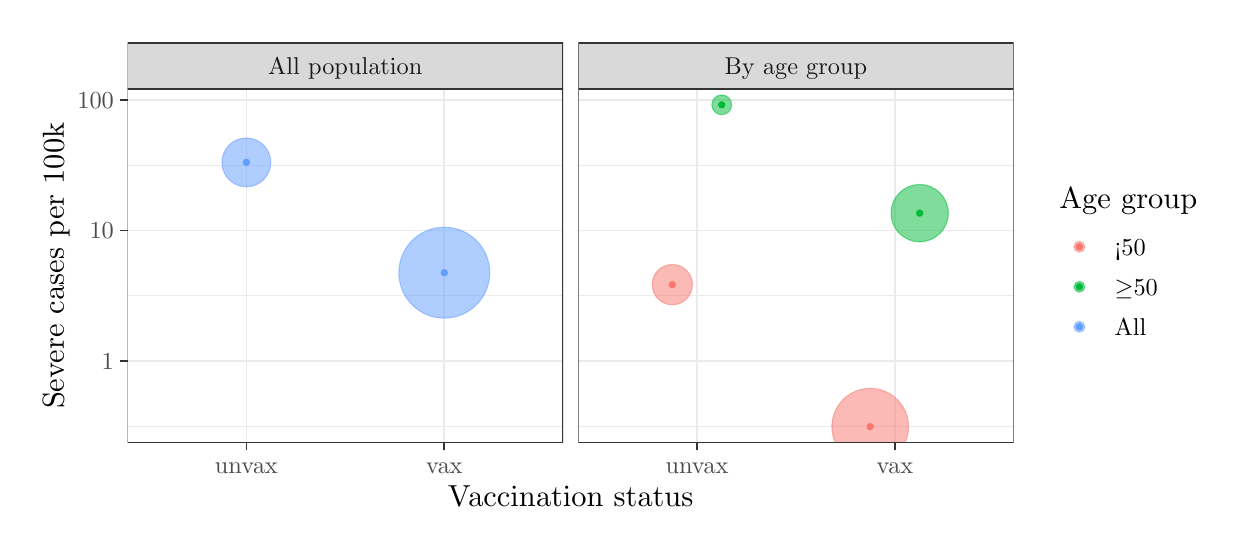
\begin{tikzpicture}[x=1pt,y=1pt]
\definecolor{fillColor}{RGB}{255,255,255}
\path[use as bounding box,fill=fillColor,fill opacity=0.00] (0,0) rectangle (433.62,180.67);
\begin{scope}
\path[clip] (  0.00,  0.00) rectangle (433.62,180.67);
\definecolor{drawColor}{RGB}{255,255,255}
\definecolor{fillColor}{RGB}{255,255,255}

\path[draw=drawColor,line width= 0.6pt,line join=round,line cap=round,fill=fillColor] (  0.00,  0.00) rectangle (433.62,180.68);
\end{scope}
\begin{scope}
\path[clip] ( 36.11, 30.69) rectangle (193.45,158.60);
\definecolor{fillColor}{RGB}{255,255,255}

\path[fill=fillColor] ( 36.11, 30.69) rectangle (193.45,158.60);
\definecolor{drawColor}{gray}{0.92}

\path[draw=drawColor,line width= 0.3pt,line join=round] ( 36.11, 36.63) --
	(193.45, 36.63);

\path[draw=drawColor,line width= 0.3pt,line join=round] ( 36.11, 83.79) --
	(193.45, 83.79);

\path[draw=drawColor,line width= 0.3pt,line join=round] ( 36.11,130.94) --
	(193.45,130.94);

\path[draw=drawColor,line width= 0.6pt,line join=round] ( 36.11, 60.21) --
	(193.45, 60.21);

\path[draw=drawColor,line width= 0.6pt,line join=round] ( 36.11,107.36) --
	(193.45,107.36);

\path[draw=drawColor,line width= 0.6pt,line join=round] ( 36.11,154.52) --
	(193.45,154.52);

\path[draw=drawColor,line width= 0.6pt,line join=round] ( 79.02, 30.69) --
	( 79.02,158.60);

\path[draw=drawColor,line width= 0.6pt,line join=round] (150.54, 30.69) --
	(150.54,158.60);
\definecolor{drawColor}{RGB}{97,156,255}
\definecolor{fillColor}{RGB}{97,156,255}

\path[draw=drawColor,draw opacity=0.50,line width= 0.4pt,line join=round,line cap=round,fill=fillColor,fill opacity=0.50] ( 79.02,131.99) circle (  8.82);

\path[draw=drawColor,draw opacity=0.50,line width= 0.4pt,line join=round,line cap=round,fill=fillColor,fill opacity=0.50] (150.54, 92.14) circle ( 16.42);
\definecolor{drawColor}{RGB}{97,156,255}
\definecolor{fillColor}{RGB}{97,156,255}

\path[draw=drawColor,line width= 0.4pt,line join=round,line cap=round,fill=fillColor] ( 79.02,131.99) circle (  1.11);

\path[draw=drawColor,line width= 0.4pt,line join=round,line cap=round,fill=fillColor] (150.54, 92.14) circle (  1.11);
\definecolor{drawColor}{gray}{0.20}

\path[draw=drawColor,line width= 0.6pt,line join=round,line cap=round] ( 36.11, 30.69) rectangle (193.45,158.60);
\end{scope}
\begin{scope}
\path[clip] (198.95, 30.69) rectangle (356.30,158.60);
\definecolor{fillColor}{RGB}{255,255,255}

\path[fill=fillColor] (198.95, 30.69) rectangle (356.30,158.60);
\definecolor{drawColor}{gray}{0.92}

\path[draw=drawColor,line width= 0.3pt,line join=round] (198.95, 36.63) --
	(356.30, 36.63);

\path[draw=drawColor,line width= 0.3pt,line join=round] (198.95, 83.79) --
	(356.30, 83.79);

\path[draw=drawColor,line width= 0.3pt,line join=round] (198.95,130.94) --
	(356.30,130.94);

\path[draw=drawColor,line width= 0.6pt,line join=round] (198.95, 60.21) --
	(356.30, 60.21);

\path[draw=drawColor,line width= 0.6pt,line join=round] (198.95,107.36) --
	(356.30,107.36);

\path[draw=drawColor,line width= 0.6pt,line join=round] (198.95,154.52) --
	(356.30,154.52);

\path[draw=drawColor,line width= 0.6pt,line join=round] (241.87, 30.69) --
	(241.87,158.60);

\path[draw=drawColor,line width= 0.6pt,line join=round] (313.38, 30.69) --
	(313.38,158.60);
\definecolor{drawColor}{RGB}{248,118,109}
\definecolor{fillColor}{RGB}{248,118,109}

\path[draw=drawColor,draw opacity=0.50,line width= 0.4pt,line join=round,line cap=round,fill=fillColor,fill opacity=0.50] (232.93, 87.82) circle (  7.27);

\path[draw=drawColor,draw opacity=0.50,line width= 0.4pt,line join=round,line cap=round,fill=fillColor,fill opacity=0.50] (304.44, 36.50) circle ( 13.83);
\definecolor{drawColor}{RGB}{0,186,56}
\definecolor{fillColor}{RGB}{0,186,56}

\path[draw=drawColor,draw opacity=0.50,line width= 0.4pt,line join=round,line cap=round,fill=fillColor,fill opacity=0.50] (250.80,152.79) circle (  3.57);

\path[draw=drawColor,draw opacity=0.50,line width= 0.4pt,line join=round,line cap=round,fill=fillColor,fill opacity=0.50] (322.32,113.65) circle ( 10.35);
\definecolor{drawColor}{RGB}{248,118,109}
\definecolor{fillColor}{RGB}{248,118,109}

\path[draw=drawColor,line width= 0.4pt,line join=round,line cap=round,fill=fillColor] (232.93, 87.82) circle (  1.11);

\path[draw=drawColor,line width= 0.4pt,line join=round,line cap=round,fill=fillColor] (304.44, 36.50) circle (  1.11);
\definecolor{drawColor}{RGB}{0,186,56}
\definecolor{fillColor}{RGB}{0,186,56}

\path[draw=drawColor,line width= 0.4pt,line join=round,line cap=round,fill=fillColor] (250.80,152.79) circle (  1.11);

\path[draw=drawColor,line width= 0.4pt,line join=round,line cap=round,fill=fillColor] (322.32,113.65) circle (  1.11);
\definecolor{drawColor}{gray}{0.20}

\path[draw=drawColor,line width= 0.6pt,line join=round,line cap=round] (198.95, 30.69) rectangle (356.30,158.60);
\end{scope}
\begin{scope}
\path[clip] ( 36.11,158.60) rectangle (193.45,175.17);
\definecolor{drawColor}{gray}{0.20}
\definecolor{fillColor}{gray}{0.85}

\path[draw=drawColor,line width= 0.6pt,line join=round,line cap=round,fill=fillColor] ( 36.11,158.60) rectangle (193.45,175.18);
\definecolor{drawColor}{gray}{0.10}

\node[text=drawColor,anchor=base,inner sep=0pt, outer sep=0pt, scale=  0.88] at (114.78,163.86) {All population};
\end{scope}
\begin{scope}
\path[clip] (198.95,158.60) rectangle (356.30,175.17);
\definecolor{drawColor}{gray}{0.20}
\definecolor{fillColor}{gray}{0.85}

\path[draw=drawColor,line width= 0.6pt,line join=round,line cap=round,fill=fillColor] (198.95,158.60) rectangle (356.30,175.18);
\definecolor{drawColor}{gray}{0.10}

\node[text=drawColor,anchor=base,inner sep=0pt, outer sep=0pt, scale=  0.88] at (277.62,163.86) {By age group};
\end{scope}
\begin{scope}
\path[clip] (  0.00,  0.00) rectangle (433.62,180.67);
\definecolor{drawColor}{gray}{0.20}

\path[draw=drawColor,line width= 0.6pt,line join=round] ( 79.02, 27.94) --
	( 79.02, 30.69);

\path[draw=drawColor,line width= 0.6pt,line join=round] (150.54, 27.94) --
	(150.54, 30.69);
\end{scope}
\begin{scope}
\path[clip] (  0.00,  0.00) rectangle (433.62,180.67);
\definecolor{drawColor}{gray}{0.30}

\node[text=drawColor,anchor=base,inner sep=0pt, outer sep=0pt, scale=  0.88] at ( 79.02, 19.68) {unvax};

\node[text=drawColor,anchor=base,inner sep=0pt, outer sep=0pt, scale=  0.88] at (150.54, 19.68) {vax};
\end{scope}
\begin{scope}
\path[clip] (  0.00,  0.00) rectangle (433.62,180.67);
\definecolor{drawColor}{gray}{0.20}

\path[draw=drawColor,line width= 0.6pt,line join=round] (241.87, 27.94) --
	(241.87, 30.69);

\path[draw=drawColor,line width= 0.6pt,line join=round] (313.38, 27.94) --
	(313.38, 30.69);
\end{scope}
\begin{scope}
\path[clip] (  0.00,  0.00) rectangle (433.62,180.67);
\definecolor{drawColor}{gray}{0.30}

\node[text=drawColor,anchor=base,inner sep=0pt, outer sep=0pt, scale=  0.88] at (241.87, 19.68) {unvax};

\node[text=drawColor,anchor=base,inner sep=0pt, outer sep=0pt, scale=  0.88] at (313.38, 19.68) {vax};
\end{scope}
\begin{scope}
\path[clip] (  0.00,  0.00) rectangle (433.62,180.67);
\definecolor{drawColor}{gray}{0.30}

\node[text=drawColor,anchor=base east,inner sep=0pt, outer sep=0pt, scale=  0.88] at ( 31.16, 57.18) {1};

\node[text=drawColor,anchor=base east,inner sep=0pt, outer sep=0pt, scale=  0.88] at ( 31.16,104.33) {10};

\node[text=drawColor,anchor=base east,inner sep=0pt, outer sep=0pt, scale=  0.88] at ( 31.16,151.49) {100};
\end{scope}
\begin{scope}
\path[clip] (  0.00,  0.00) rectangle (433.62,180.67);
\definecolor{drawColor}{gray}{0.20}

\path[draw=drawColor,line width= 0.6pt,line join=round] ( 33.36, 60.21) --
	( 36.11, 60.21);

\path[draw=drawColor,line width= 0.6pt,line join=round] ( 33.36,107.36) --
	( 36.11,107.36);

\path[draw=drawColor,line width= 0.6pt,line join=round] ( 33.36,154.52) --
	( 36.11,154.52);
\end{scope}
\begin{scope}
\path[clip] (  0.00,  0.00) rectangle (433.62,180.67);
\definecolor{drawColor}{RGB}{0,0,0}

\node[text=drawColor,anchor=base,inner sep=0pt, outer sep=0pt, scale=  1.10] at (196.20,  7.64) {Vaccination status};
\end{scope}
\begin{scope}
\path[clip] (  0.00,  0.00) rectangle (433.62,180.67);
\definecolor{drawColor}{RGB}{0,0,0}

\node[text=drawColor,rotate= 90.00,anchor=base,inner sep=0pt, outer sep=0pt, scale=  1.10] at ( 13.08, 94.64) {Severe cases per 100k};
\end{scope}
\begin{scope}
\path[clip] (  0.00,  0.00) rectangle (433.62,180.67);
\definecolor{fillColor}{RGB}{255,255,255}

\path[fill=fillColor] (367.30, 59.86) rectangle (428.12,129.43);
\end{scope}
\begin{scope}
\path[clip] (  0.00,  0.00) rectangle (433.62,180.67);
\definecolor{drawColor}{RGB}{0,0,0}

\node[text=drawColor,anchor=base west,inner sep=0pt, outer sep=0pt, scale=  1.10] at (372.80,115.29) {Age group};
\end{scope}
\begin{scope}
\path[clip] (  0.00,  0.00) rectangle (433.62,180.67);
\definecolor{fillColor}{RGB}{255,255,255}

\path[fill=fillColor] (372.80, 94.26) rectangle (387.25,108.72);
\end{scope}
\begin{scope}
\path[clip] (  0.00,  0.00) rectangle (433.62,180.67);
\definecolor{drawColor}{RGB}{248,118,109}
\definecolor{fillColor}{RGB}{248,118,109}

\path[draw=drawColor,draw opacity=0.50,line width= 0.4pt,line join=round,line cap=round,fill=fillColor,fill opacity=0.50] (380.02,101.49) circle (  1.96);
\end{scope}
\begin{scope}
\path[clip] (  0.00,  0.00) rectangle (433.62,180.67);
\definecolor{drawColor}{RGB}{248,118,109}
\definecolor{fillColor}{RGB}{248,118,109}

\path[draw=drawColor,line width= 0.4pt,line join=round,line cap=round,fill=fillColor] (380.02,101.49) circle (  1.11);
\end{scope}
\begin{scope}
\path[clip] (  0.00,  0.00) rectangle (433.62,180.67);
\definecolor{fillColor}{RGB}{255,255,255}

\path[fill=fillColor] (372.80, 79.81) rectangle (387.25, 94.26);
\end{scope}
\begin{scope}
\path[clip] (  0.00,  0.00) rectangle (433.62,180.67);
\definecolor{drawColor}{RGB}{0,186,56}
\definecolor{fillColor}{RGB}{0,186,56}

\path[draw=drawColor,draw opacity=0.50,line width= 0.4pt,line join=round,line cap=round,fill=fillColor,fill opacity=0.50] (380.02, 87.04) circle (  1.96);
\end{scope}
\begin{scope}
\path[clip] (  0.00,  0.00) rectangle (433.62,180.67);
\definecolor{drawColor}{RGB}{0,186,56}
\definecolor{fillColor}{RGB}{0,186,56}

\path[draw=drawColor,line width= 0.4pt,line join=round,line cap=round,fill=fillColor] (380.02, 87.04) circle (  1.11);
\end{scope}
\begin{scope}
\path[clip] (  0.00,  0.00) rectangle (433.62,180.67);
\definecolor{fillColor}{RGB}{255,255,255}

\path[fill=fillColor] (372.80, 65.36) rectangle (387.25, 79.81);
\end{scope}
\begin{scope}
\path[clip] (  0.00,  0.00) rectangle (433.62,180.67);
\definecolor{drawColor}{RGB}{97,156,255}
\definecolor{fillColor}{RGB}{97,156,255}

\path[draw=drawColor,draw opacity=0.50,line width= 0.4pt,line join=round,line cap=round,fill=fillColor,fill opacity=0.50] (380.02, 72.58) circle (  1.96);
\end{scope}
\begin{scope}
\path[clip] (  0.00,  0.00) rectangle (433.62,180.67);
\definecolor{drawColor}{RGB}{97,156,255}
\definecolor{fillColor}{RGB}{97,156,255}

\path[draw=drawColor,line width= 0.4pt,line join=round,line cap=round,fill=fillColor] (380.02, 72.58) circle (  1.11);
\end{scope}
\begin{scope}
\path[clip] (  0.00,  0.00) rectangle (433.62,180.67);
\definecolor{drawColor}{RGB}{0,0,0}

\node[text=drawColor,anchor=base west,inner sep=0pt, outer sep=0pt, scale=  0.88] at (392.75, 98.46) {<50};
\end{scope}
\begin{scope}
\path[clip] (  0.00,  0.00) rectangle (433.62,180.67);
\definecolor{drawColor}{RGB}{0,0,0}

\node[text=drawColor,anchor=base west,inner sep=0pt, outer sep=0pt, scale=  0.88] at (392.75, 84.01) {$\geq$50};
\end{scope}
\begin{scope}
\path[clip] (  0.00,  0.00) rectangle (433.62,180.67);
\definecolor{drawColor}{RGB}{0,0,0}

\node[text=drawColor,anchor=base west,inner sep=0pt, outer sep=0pt, scale=  0.88] at (392.75, 69.55) {All};
\end{scope}
\end{tikzpicture}
}
  \end{figure}

\end{frame}

% ─────────────────────────────────────────────────────────────────────────────

\begin{frame}{Balanced Data}

  \begin{center}

    \onslide<1>{{\bfseries \Large Confounding}}

    \bs

    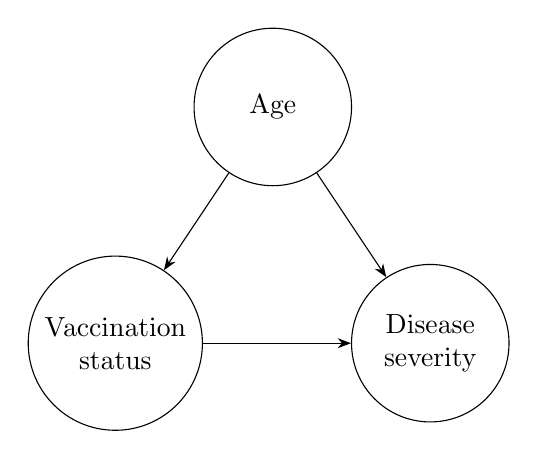
\begin{tikzpicture}[>=Stealth]

      % Set common node style
      \tikzset{
        mynode/.style={draw, circle, minimum size=2cm, align=center},
      }

      % Nodes
      \node (exposure) [mynode] at (0,0) {Vaccination\\status};
      \node (outcome) [mynode] at (4,0) {Disease\\severity};
      \node (confounder) [mynode] at (2,3) {Age};

      % Arrows
      \draw[->] (exposure) -- (outcome);
      \draw[->] (confounder) -- (outcome);
      \onslide<1>{
        \draw[->] (confounder) -- (exposure);
      }

    \end{tikzpicture}

    \bs

    \onslide<2>{{\bfseries Balancing the data removed the confounding.}}

  \end{center}

\end{frame}

% ─────────────────────────────────────────────────────────────────────────────

\begin{frame}{Treatments for Kidney Stones}

  \begin{minipage}{0.8\textwidth}

    
\includegraphics[width=\textwidth]{images/charig1986_title.png}

  \end{minipage}%
  %
  \begin{minipage}{0.2\textwidth}
    \href{\charigURL}{
      \small
      Charig et al. \\
      Br Med J (Clin Res Ed) \\
      1986
    }
  \end{minipage}

  \begin{minipage}[t]{0.25\textwidth}

    {\bfseries Open Surgery}

    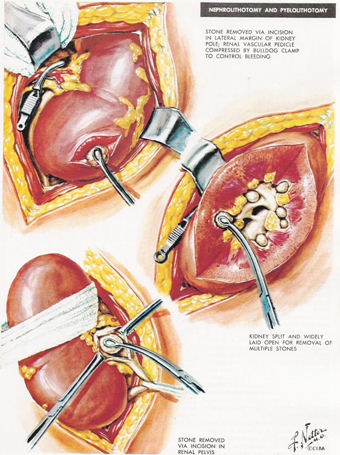
\includegraphics[width=\textwidth]{images/open_surgery.jpg}

  \end{minipage}%
  %
  \begin{minipage}[t]{0.35\textwidth}

    {\bfseries Percutaneous Nephrolithotomy}

    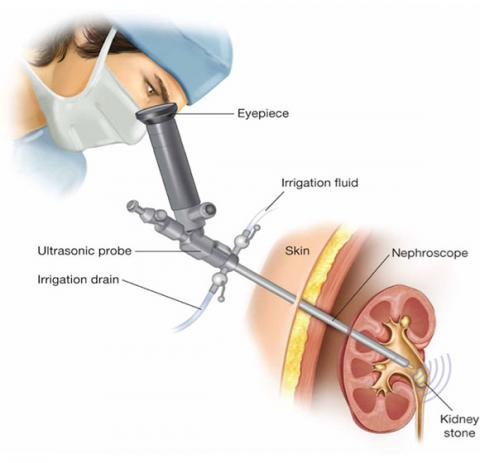
\includegraphics[width=\textwidth]{images/percutaneous-nephrolithotomy.jpg}

  \end{minipage}%
  %
  \begin{minipage}[t]{0.4\textwidth}

    {\bfseries Extracorporeal Shock Wave Lithotripsy}

    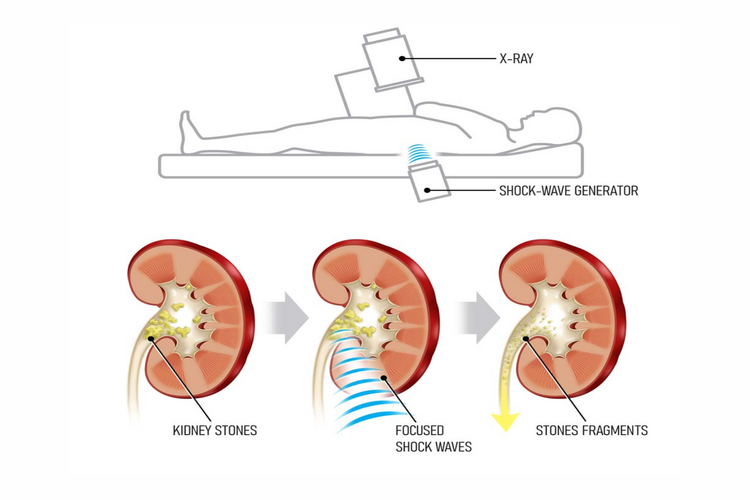
\includegraphics[width=\textwidth]{%
      images/extracorporeal_shock_wave_lithotripsy.png}

    \end{minipage}

\end{frame}

% ─────────────────────────────────────────────────────────────────────────────

\begin{frame}{Kidney Stones Data}

  % |surgery |stone_size |   n| success| failure| rate|
  % |:-------|:----------|---:|-------:|-------:|----:|
  % |open    |small      |  87|      81|       6| 0.93|
  % |pcnl    |small      | 270|     234|      36| 0.87|
  % |open    |large      | 263|     192|      71| 0.73|
  % |pcnl    |large      |  80|      55|      25| 0.69|
  % |open    |overall    | 350|     273|      77| 0.78|
  % |pcnl    |overall    | 350|     289|      61| 0.83|

  \begin{minipage}{.6\textwidth}

    {\bfseries Data from the Article:}

    \bs

    % latex table generated in R 4.4.1 by xtable 1.8-4 package
% Wed Oct 23 19:35:16 2024
\begin{table}[ht]
\centering
\begin{tabular}{llrrrr}
  \toprule
{\textbf{Surgery}} & {\textbf{Stone Size}} & {\textbf{N}} & {\textbf{Success}} & {\textbf{Failure}} & {\textbf{Rate}} \\ 
  \midrule
open & small &  87 &  81 &   6 & 0.93 \\ 
  pcnl & small & 270 & 234 &  36 & 0.87 \\ 
  open & large & 263 & 192 &  71 & 0.73 \\ 
  pcnl & large &  80 &  55 &  25 & 0.69 \\ 
  open & overall & 350 & 273 &  77 & 0.78 \\ 
  pcnl & overall & 350 & 289 &  61 & 0.83 \\ 
   \bottomrule
\end{tabular}
\end{table}


  \end{minipage}%
  %
  \begin{minipage}{.4\textwidth}

    \centering

    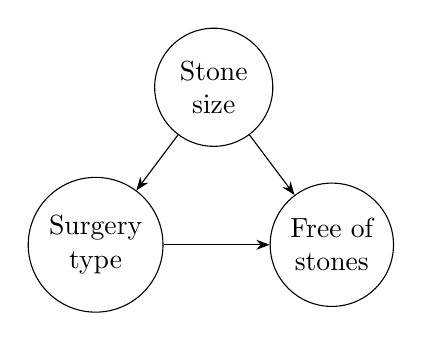
\begin{tikzpicture}[>=Stealth]
      % Node style
      \tikzset{
        mynode/.style={draw, circle, minimum size=1.5cm, align=center},
      }
      % Nodes
      \node (exposure) [mynode] at (0,0) {Surgery\\type};
      \node (outcome) [mynode] at (3,0) {Free of\\stones};
      \node (confounder) [mynode] at (1.5,2) {Stone\\size};
      % Arrows
      \draw[->] (exposure) -- (outcome);
      \draw[->] (confounder) -- (outcome);
      \draw[->] (confounder) -- (exposure);
    \end{tikzpicture}

  \end{minipage}

  \bs

  {\bfseries Statistics (Risk):}

  \bs

  % +--------+---------+---------+------------+-------+--------+
  % |stone   | success | success | risk       | risk  | odds   |
  % |size    | open    | pcnl    | difference | ratio | ratios |
  % +--------+---------+---------+------------+-------+--------+
  % |small   | 81/87   | 234/270 | -0.06      | 0.93  | 0.48   |
  % +--------+---------+---------+------------+-------+--------+
  % |large   | 192/263 | 55/80   | -0.04      | 0.94  | 0.81   |
  % +--------+---------+---------+------------+-------+--------+
  % |overall | 273/350 | 289/350 |  0.05      | 1.06  | 1.34   |
  % +--------+---------+---------+------------+-------+--------+

  % latex table generated in R 4.4.1 by xtable 1.8-4 package
% Wed Oct 23 19:35:16 2024
\begin{table}[ht]
\centering
\begin{tabular}{lllrrr}
  \toprule
{\textbf{Stone Size}} & {\textbf{Success Open}} & {\textbf{Success PCNL}} & {\textbf{Risk Difference}} & {\textbf{Risk Ratio}} & {\textbf{Odds Ratio}} \\ 
  \midrule
small & 81/87 & 234/270 & -0.06 & 0.93 & 0.48 \\ 
  large & 192/263 & 55/80 & -0.04 & 0.94 & 0.81 \\ 
  overall & 273/350 & 289/350 & 0.05 & 1.06 & 1.34 \\ 
   \bottomrule
\end{tabular}
\end{table}


\end{frame}

% ─────────────────────────────────────────────────────────────────────────────

\begin{frame}{Kidney Stones Data - Balanced}

  \begin{minipage}{.6\textwidth}

    {\bfseries Balanced Data:}

    \vspace{.5\baselineskip}

    {
      \small
      (Keep the rate in groups, balance the data, and recalculate the number of
      successes and failures.)
    }

    \vspace{.35\baselineskip}

    % latex table generated in R 4.4.1 by xtable 1.8-4 package
% Wed Oct 23 19:35:16 2024
\begin{table}[ht]
\centering
\begin{tabular}{llrrrr}
  \toprule
{\textbf{Surgery}} & {\textbf{Stone Size}} & {\textbf{N}} & {\textbf{Success}} & {\textbf{Failure}} & {\textbf{Rate}} \\ 
  \midrule
open & small & 175.00 & 163.00 & 12.00 & 0.93 \\ 
  pcnl & small & 175.00 & 152.00 & 23.00 & 0.87 \\ 
  open & large & 175.00 & 128.00 & 47.00 & 0.73 \\ 
  pcnl & large & 175.00 & 120.00 & 55.00 & 0.69 \\ 
  open & overall & 350.00 & 291.00 & 59.00 & 0.83 \\ 
  pcnl & overall & 350.00 & 272.00 & 78.00 & 0.78 \\ 
   \bottomrule
\end{tabular}
\end{table}


  \end{minipage}%
  %
  \begin{minipage}{.4\textwidth}

    \centering

    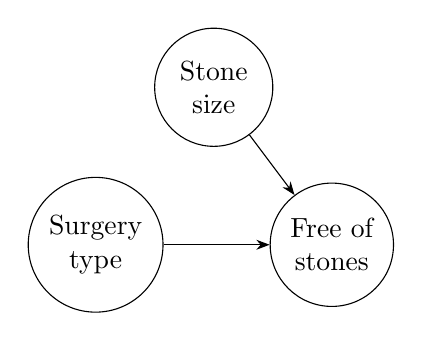
\begin{tikzpicture}[>=Stealth]
      % Node style
      \tikzset{
        mynode/.style={draw, circle, minimum size=1.5cm, align=center},
      }
      % Nodes
      \node (exposure) [mynode] at (0,0) {Surgery\\type};
      \node (outcome) [mynode] at (3,0) {Free of\\stones};
      \node (confounder) [mynode] at (1.5,2) {Stone\\size};
      % Arrows
      \draw[->] (exposure) -- (outcome);
      \draw[->] (confounder) -- (outcome);
    \end{tikzpicture}

  \end{minipage}

  \bs

  {\bfseries Statistics (Risk):}

  \bs

  % latex table generated in R 4.4.1 by xtable 1.8-4 package
% Wed Oct 23 19:35:16 2024
\begin{table}[ht]
\centering
\begin{tabular}{lllrrr}
  \toprule
{\textbf{Stone Size}} & {\textbf{Success Open}} & {\textbf{Success PCNL}} & {\textbf{Risk Difference}} & {\textbf{Risk Ratio}} & {\textbf{Odds Ratio}} \\ 
  \midrule
small & 163/175 & 152/175 & -0.06 & 0.93 & 0.49 \\ 
  large & 128/175 & 120/175 & -0.05 & 0.94 & 0.80 \\ 
  overall & 291/350 & 272/350 & -0.05 & 0.93 & 0.71 \\ 
   \bottomrule
\end{tabular}
\end{table}


\end{frame}

% ─────────────────────────────────────────────────────────────────────────────

\begin{frame}{Kidney Stones Data - Logistic Regression}

  {\bfseries Model 1:}
  %
  \(
    \logit(\text{free of stones}) = \beta_0 + \beta_1 \times
    \text{surgery type}
  \)

  \bs

  {\bfseries Model 2:}
  %
  \(
    \logit(\text{free of stones}) = \beta_0 + \beta_1 \times
    \text{surgery type} + \beta_2 \times \text{stone size}
  \)

  \bs \bs

  \begin{minipage}[t]{.5\textwidth}

    \centering

    {\bfseries Original Data, Model 1}

    % latex table generated in R 4.4.1 by xtable 1.8-4 package
% Wed Oct 23 19:35:16 2024
\begin{table}[ht]
\centering
\begin{tabular}{lrrr}
  \toprule
{\textbf{Term}} & {\textbf{OR}} & {\textbf{2.5\%}} & {\textbf{97.5\%}} \\ 
  \midrule
(Intercept) & 3.55 & 2.77 & 4.59 \\ 
  PCNL Surgery & 1.34 & 0.92 & 1.95 \\ 
   \bottomrule
\end{tabular}
\end{table}


  \end{minipage}%
  %
  \begin{minipage}[t]{.5\textwidth}

    \centering

    {\bfseries Original Data, Model 2}

    % latex table generated in R 4.4.1 by xtable 1.8-4 package
% Wed Oct 23 19:35:16 2024
\begin{table}[ht]
\centering
\begin{tabular}{lrrr}
  \toprule
{\textbf{Term}} & {\textbf{OR}} & {\textbf{2.5\%}} & {\textbf{97.5\%}} \\ 
  \midrule
(Intercept) & 2.81 & 2.17 & 3.68 \\ 
  PCNL Surgery & 0.70 & 0.45 & 1.09 \\ 
  Small Stone & 3.53 & 2.22 & 5.68 \\ 
   \bottomrule
\end{tabular}
\end{table}


  \end{minipage}

  \bs

  \begin{minipage}[t]{.5\textwidth}

    \centering

    {\bfseries Balanced Data, Model 1}

    % latex table generated in R 4.4.1 by xtable 1.8-4 package
% Wed Oct 23 19:35:16 2024
\begin{table}[ht]
\centering
\begin{tabular}{lrrr}
  \toprule
{\textbf{Term}} & {\textbf{OR}} & {\textbf{2.5\%}} & {\textbf{97.5\%}} \\ 
  \midrule
(Intercept) & 4.93 & 3.76 & 6.59 \\ 
  PCNL Surgery & 0.71 & 0.48 & 1.03 \\ 
   \bottomrule
\end{tabular}
\end{table}


  \end{minipage}%
  %
  \begin{minipage}[t]{.5\textwidth}

    \centering

    {\bfseries Balanced Data, Model 2}

    % latex table generated in R 4.4.1 by xtable 1.8-4 package
% Wed Oct 23 19:35:16 2024
\begin{table}[ht]
\centering
\begin{tabular}{lrrr}
  \toprule
{\textbf{Term}} & {\textbf{OR}} & {\textbf{2.5\%}} & {\textbf{97.5\%}} \\ 
  \midrule
(Intercept) & 2.94 & 2.17 & 4.05 \\ 
  PCNL Surgery & 0.69 & 0.47 & 1.02 \\ 
  Small Stone & 3.73 & 2.47 & 5.73 \\ 
   \bottomrule
\end{tabular}
\end{table}


  \end{minipage}

\end{frame}

% ─────────────────────────────────────────────────────────────────────────────

% \begin{frame}{Moderation in balanced data}
%
% \end{frame}

% ─────────────────────────────────────────────────────────────────────────────

\begin{frame}{Latest Example (Seen on an ARTE Program)}

  \begin{minipage}{.5\textwidth}

    \onslide<1->

    \begin{figure}[!h]
      \centering
      \resizebox{.9\columnwidth}{!}{% Created by tikzDevice version 0.12.6 on 2024-10-23 19:35:38
% !TEX encoding = UTF-8 Unicode
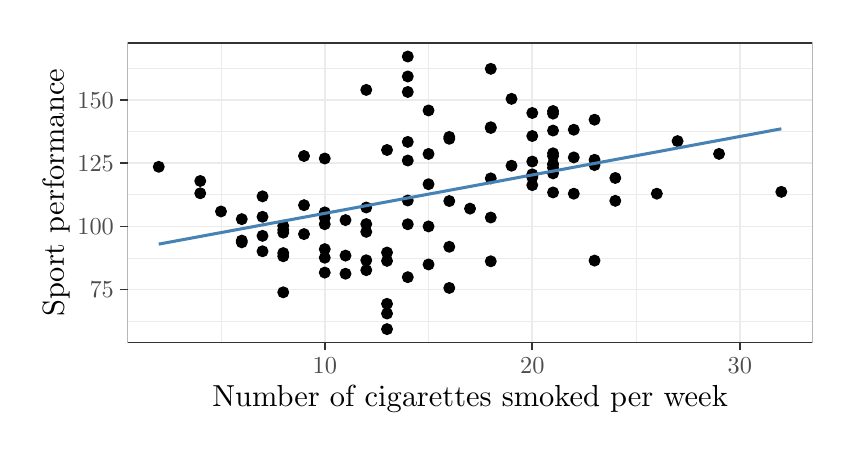
\begin{tikzpicture}[x=1pt,y=1pt]
\definecolor{fillColor}{RGB}{255,255,255}
\path[use as bounding box,fill=fillColor,fill opacity=0.00] (0,0) rectangle (289.08,144.54);
\begin{scope}
\path[clip] (  0.00,  0.00) rectangle (289.08,144.54);
\definecolor{drawColor}{RGB}{255,255,255}
\definecolor{fillColor}{RGB}{255,255,255}

\path[draw=drawColor,line width= 0.6pt,line join=round,line cap=round,fill=fillColor] (  0.00,  0.00) rectangle (289.08,144.54);
\end{scope}
\begin{scope}
\path[clip] ( 36.11, 30.69) rectangle (283.58,139.04);
\definecolor{fillColor}{RGB}{255,255,255}

\path[fill=fillColor] ( 36.11, 30.69) rectangle (283.58,139.04);
\definecolor{drawColor}{gray}{0.92}

\path[draw=drawColor,line width= 0.3pt,line join=round] ( 36.11, 38.47) --
	(283.58, 38.47);

\path[draw=drawColor,line width= 0.3pt,line join=round] ( 36.11, 61.31) --
	(283.58, 61.31);

\path[draw=drawColor,line width= 0.3pt,line join=round] ( 36.11, 84.15) --
	(283.58, 84.15);

\path[draw=drawColor,line width= 0.3pt,line join=round] ( 36.11,107.00) --
	(283.58,107.00);

\path[draw=drawColor,line width= 0.3pt,line join=round] ( 36.11,129.84) --
	(283.58,129.84);

\path[draw=drawColor,line width= 0.3pt,line join=round] ( 69.86, 30.69) --
	( 69.86,139.04);

\path[draw=drawColor,line width= 0.3pt,line join=round] (144.85, 30.69) --
	(144.85,139.04);

\path[draw=drawColor,line width= 0.3pt,line join=round] (219.84, 30.69) --
	(219.84,139.04);

\path[draw=drawColor,line width= 0.6pt,line join=round] ( 36.11, 49.89) --
	(283.58, 49.89);

\path[draw=drawColor,line width= 0.6pt,line join=round] ( 36.11, 72.73) --
	(283.58, 72.73);

\path[draw=drawColor,line width= 0.6pt,line join=round] ( 36.11, 95.57) --
	(283.58, 95.57);

\path[draw=drawColor,line width= 0.6pt,line join=round] ( 36.11,118.42) --
	(283.58,118.42);

\path[draw=drawColor,line width= 0.6pt,line join=round] (107.35, 30.69) --
	(107.35,139.04);

\path[draw=drawColor,line width= 0.6pt,line join=round] (182.34, 30.69) --
	(182.34,139.04);

\path[draw=drawColor,line width= 0.6pt,line join=round] (257.33, 30.69) --
	(257.33,139.04);
\definecolor{drawColor}{RGB}{0,0,0}
\definecolor{fillColor}{RGB}{0,0,0}

\path[draw=drawColor,line width= 0.4pt,line join=round,line cap=round,fill=fillColor] (122.35, 70.76) circle (  1.96);

\path[draw=drawColor,line width= 0.4pt,line join=round,line cap=round,fill=fillColor] (152.35, 65.36) circle (  1.96);

\path[draw=drawColor,line width= 0.4pt,line join=round,line cap=round,fill=fillColor] ( 92.35, 71.51) circle (  1.96);

\path[draw=drawColor,line width= 0.4pt,line join=round,line cap=round,fill=fillColor] (152.35, 81.89) circle (  1.96);

\path[draw=drawColor,line width= 0.4pt,line join=round,line cap=round,fill=fillColor] ( 47.36, 94.26) circle (  1.96);

\path[draw=drawColor,line width= 0.4pt,line join=round,line cap=round,fill=fillColor] (167.34, 60.12) circle (  1.96);

\path[draw=drawColor,line width= 0.4pt,line join=round,line cap=round,fill=fillColor] ( 62.36, 89.14) circle (  1.96);

\path[draw=drawColor,line width= 0.4pt,line join=round,line cap=round,fill=fillColor] ( 92.35, 48.91) circle (  1.96);

\path[draw=drawColor,line width= 0.4pt,line join=round,line cap=round,fill=fillColor] (107.35, 61.41) circle (  1.96);

\path[draw=drawColor,line width= 0.4pt,line join=round,line cap=round,fill=fillColor] (129.85, 41.24) circle (  1.96);

\path[draw=drawColor,line width= 0.4pt,line join=round,line cap=round,fill=fillColor] ( 99.85, 69.95) circle (  1.96);

\path[draw=drawColor,line width= 0.4pt,line join=round,line cap=round,fill=fillColor] (107.35, 73.52) circle (  1.96);

\path[draw=drawColor,line width= 0.4pt,line join=round,line cap=round,fill=fillColor] ( 99.85, 80.40) circle (  1.96);

\path[draw=drawColor,line width= 0.4pt,line join=round,line cap=round,fill=fillColor] (137.35, 54.38) circle (  1.96);

\path[draw=drawColor,line width= 0.4pt,line join=round,line cap=round,fill=fillColor] (107.35, 77.80) circle (  1.96);

\path[draw=drawColor,line width= 0.4pt,line join=round,line cap=round,fill=fillColor] (107.35, 75.81) circle (  1.96);

\path[draw=drawColor,line width= 0.4pt,line join=round,line cap=round,fill=fillColor] (152.35, 50.49) circle (  1.96);

\path[draw=drawColor,line width= 0.4pt,line join=round,line cap=round,fill=fillColor] (122.35, 73.57) circle (  1.96);

\path[draw=drawColor,line width= 0.4pt,line join=round,line cap=round,fill=fillColor] (107.35, 64.51) circle (  1.96);

\path[draw=drawColor,line width= 0.4pt,line join=round,line cap=round,fill=fillColor] (159.85, 79.15) circle (  1.96);

\path[draw=drawColor,line width= 0.4pt,line join=round,line cap=round,fill=fillColor] ( 69.86, 78.13) circle (  1.96);

\path[draw=drawColor,line width= 0.4pt,line join=round,line cap=round,fill=fillColor] (144.85, 58.98) circle (  1.96);

\path[draw=drawColor,line width= 0.4pt,line join=round,line cap=round,fill=fillColor] (122.35, 56.92) circle (  1.96);

\path[draw=drawColor,line width= 0.4pt,line join=round,line cap=round,fill=fillColor] (114.85, 55.63) circle (  1.96);

\path[draw=drawColor,line width= 0.4pt,line join=round,line cap=round,fill=fillColor] ( 92.35, 61.94) circle (  1.96);

\path[draw=drawColor,line width= 0.4pt,line join=round,line cap=round,fill=fillColor] (137.35, 82.09) circle (  1.96);

\path[draw=drawColor,line width= 0.4pt,line join=round,line cap=round,fill=fillColor] (137.35, 73.50) circle (  1.96);

\path[draw=drawColor,line width= 0.4pt,line join=round,line cap=round,fill=fillColor] ( 92.35, 72.92) circle (  1.96);

\path[draw=drawColor,line width= 0.4pt,line join=round,line cap=round,fill=fillColor] (129.85, 44.75) circle (  1.96);

\path[draw=drawColor,line width= 0.4pt,line join=round,line cap=round,fill=fillColor] (122.35, 60.49) circle (  1.96);

\path[draw=drawColor,line width= 0.4pt,line join=round,line cap=round,fill=fillColor] ( 62.36, 84.70) circle (  1.96);

\path[draw=drawColor,line width= 0.4pt,line join=round,line cap=round,fill=fillColor] (122.35, 79.56) circle (  1.96);

\path[draw=drawColor,line width= 0.4pt,line join=round,line cap=round,fill=fillColor] ( 92.35, 70.46) circle (  1.96);

\path[draw=drawColor,line width= 0.4pt,line join=round,line cap=round,fill=fillColor] ( 92.35, 63.09) circle (  1.96);

\path[draw=drawColor,line width= 0.4pt,line join=round,line cap=round,fill=fillColor] (144.85, 72.72) circle (  1.96);

\path[draw=drawColor,line width= 0.4pt,line join=round,line cap=round,fill=fillColor] (114.85, 62.18) circle (  1.96);

\path[draw=drawColor,line width= 0.4pt,line join=round,line cap=round,fill=fillColor] ( 77.36, 75.35) circle (  1.96);

\path[draw=drawColor,line width= 0.4pt,line join=round,line cap=round,fill=fillColor] (107.35, 97.26) circle (  1.96);

\path[draw=drawColor,line width= 0.4pt,line join=round,line cap=round,fill=fillColor] ( 77.36, 67.60) circle (  1.96);

\path[draw=drawColor,line width= 0.4pt,line join=round,line cap=round,fill=fillColor] (114.85, 75.01) circle (  1.96);

\path[draw=drawColor,line width= 0.4pt,line join=round,line cap=round,fill=fillColor] (107.35, 56.04) circle (  1.96);

\path[draw=drawColor,line width= 0.4pt,line join=round,line cap=round,fill=fillColor] (129.85, 60.28) circle (  1.96);

\path[draw=drawColor,line width= 0.4pt,line join=round,line cap=round,fill=fillColor] ( 84.86, 83.59) circle (  1.96);

\path[draw=drawColor,line width= 0.4pt,line join=round,line cap=round,fill=fillColor] ( 84.86, 76.20) circle (  1.96);

\path[draw=drawColor,line width= 0.4pt,line join=round,line cap=round,fill=fillColor] ( 84.86, 69.32) circle (  1.96);

\path[draw=drawColor,line width= 0.4pt,line join=round,line cap=round,fill=fillColor] ( 99.85, 98.17) circle (  1.96);

\path[draw=drawColor,line width= 0.4pt,line join=round,line cap=round,fill=fillColor] (129.85, 35.61) circle (  1.96);

\path[draw=drawColor,line width= 0.4pt,line join=round,line cap=round,fill=fillColor] ( 84.86, 63.73) circle (  1.96);

\path[draw=drawColor,line width= 0.4pt,line join=round,line cap=round,fill=fillColor] ( 77.36, 66.97) circle (  1.96);

\path[draw=drawColor,line width= 0.4pt,line join=round,line cap=round,fill=fillColor] (129.85, 63.29) circle (  1.96);

\path[draw=drawColor,line width= 0.4pt,line join=round,line cap=round,fill=fillColor] (189.84, 85.00) circle (  1.96);

\path[draw=drawColor,line width= 0.4pt,line join=round,line cap=round,fill=fillColor] (272.33, 85.21) circle (  1.96);

\path[draw=drawColor,line width= 0.4pt,line join=round,line cap=round,fill=fillColor] (182.34, 87.64) circle (  1.96);

\path[draw=drawColor,line width= 0.4pt,line join=round,line cap=round,fill=fillColor] (189.84,107.36) circle (  1.96);

\path[draw=drawColor,line width= 0.4pt,line join=round,line cap=round,fill=fillColor] (234.84,103.55) circle (  1.96);

\path[draw=drawColor,line width= 0.4pt,line join=round,line cap=round,fill=fillColor] (174.84,118.82) circle (  1.96);

\path[draw=drawColor,line width= 0.4pt,line join=round,line cap=round,fill=fillColor] (167.34, 75.94) circle (  1.96);

\path[draw=drawColor,line width= 0.4pt,line join=round,line cap=round,fill=fillColor] (174.84, 94.66) circle (  1.96);

\path[draw=drawColor,line width= 0.4pt,line join=round,line cap=round,fill=fillColor] (204.84,111.28) circle (  1.96);

\path[draw=drawColor,line width= 0.4pt,line join=round,line cap=round,fill=fillColor] (182.34, 90.44) circle (  1.96);

\path[draw=drawColor,line width= 0.4pt,line join=round,line cap=round,fill=fillColor] (137.35,103.26) circle (  1.96);

\path[draw=drawColor,line width= 0.4pt,line join=round,line cap=round,fill=fillColor] (167.34,108.57) circle (  1.96);

\path[draw=drawColor,line width= 0.4pt,line join=round,line cap=round,fill=fillColor] (182.34,105.39) circle (  1.96);

\path[draw=drawColor,line width= 0.4pt,line join=round,line cap=round,fill=fillColor] (197.34,107.66) circle (  1.96);

\path[draw=drawColor,line width= 0.4pt,line join=round,line cap=round,fill=fillColor] (144.85,114.63) circle (  1.96);

\path[draw=drawColor,line width= 0.4pt,line join=round,line cap=round,fill=fillColor] (227.34, 84.55) circle (  1.96);

\path[draw=drawColor,line width= 0.4pt,line join=round,line cap=round,fill=fillColor] (204.84, 60.38) circle (  1.96);

\path[draw=drawColor,line width= 0.4pt,line join=round,line cap=round,fill=fillColor] (167.34,108.29) circle (  1.96);

\path[draw=drawColor,line width= 0.4pt,line join=round,line cap=round,fill=fillColor] (137.35,134.11) circle (  1.96);

\path[draw=drawColor,line width= 0.4pt,line join=round,line cap=round,fill=fillColor] (204.84, 94.89) circle (  1.96);

\path[draw=drawColor,line width= 0.4pt,line join=round,line cap=round,fill=fillColor] (189.84, 99.15) circle (  1.96);

\path[draw=drawColor,line width= 0.4pt,line join=round,line cap=round,fill=fillColor] (152.35,105.06) circle (  1.96);

\path[draw=drawColor,line width= 0.4pt,line join=round,line cap=round,fill=fillColor] (182.34, 91.08) circle (  1.96);

\path[draw=drawColor,line width= 0.4pt,line join=round,line cap=round,fill=fillColor] (137.35,121.31) circle (  1.96);

\path[draw=drawColor,line width= 0.4pt,line join=round,line cap=round,fill=fillColor] (137.35,126.91) circle (  1.96);

\path[draw=drawColor,line width= 0.4pt,line join=round,line cap=round,fill=fillColor] (189.84, 95.17) circle (  1.96);

\path[draw=drawColor,line width= 0.4pt,line join=round,line cap=round,fill=fillColor] (189.84, 91.90) circle (  1.96);

\path[draw=drawColor,line width= 0.4pt,line join=round,line cap=round,fill=fillColor] (144.85, 98.91) circle (  1.96);

\path[draw=drawColor,line width= 0.4pt,line join=round,line cap=round,fill=fillColor] (189.84,114.42) circle (  1.96);

\path[draw=drawColor,line width= 0.4pt,line join=round,line cap=round,fill=fillColor] (129.85,100.34) circle (  1.96);

\path[draw=drawColor,line width= 0.4pt,line join=round,line cap=round,fill=fillColor] (182.34, 91.54) circle (  1.96);

\path[draw=drawColor,line width= 0.4pt,line join=round,line cap=round,fill=fillColor] (182.34,113.71) circle (  1.96);

\path[draw=drawColor,line width= 0.4pt,line join=round,line cap=round,fill=fillColor] (249.83, 98.93) circle (  1.96);

\path[draw=drawColor,line width= 0.4pt,line join=round,line cap=round,fill=fillColor] (182.34, 96.16) circle (  1.96);

\path[draw=drawColor,line width= 0.4pt,line join=round,line cap=round,fill=fillColor] (167.34,129.67) circle (  1.96);

\path[draw=drawColor,line width= 0.4pt,line join=round,line cap=round,fill=fillColor] (189.84,113.48) circle (  1.96);

\path[draw=drawColor,line width= 0.4pt,line join=round,line cap=round,fill=fillColor] (212.34, 90.23) circle (  1.96);

\path[draw=drawColor,line width= 0.4pt,line join=round,line cap=round,fill=fillColor] (137.35, 96.53) circle (  1.96);

\path[draw=drawColor,line width= 0.4pt,line join=round,line cap=round,fill=fillColor] (152.35,104.38) circle (  1.96);

\path[draw=drawColor,line width= 0.4pt,line join=round,line cap=round,fill=fillColor] (189.84, 95.21) circle (  1.96);

\path[draw=drawColor,line width= 0.4pt,line join=round,line cap=round,fill=fillColor] (204.84, 96.80) circle (  1.96);

\path[draw=drawColor,line width= 0.4pt,line join=round,line cap=round,fill=fillColor] (144.85, 87.97) circle (  1.96);

\path[draw=drawColor,line width= 0.4pt,line join=round,line cap=round,fill=fillColor] (167.34, 90.09) circle (  1.96);

\path[draw=drawColor,line width= 0.4pt,line join=round,line cap=round,fill=fillColor] (212.34, 81.97) circle (  1.96);

\path[draw=drawColor,line width= 0.4pt,line join=round,line cap=round,fill=fillColor] (122.35,122.05) circle (  1.96);

\path[draw=drawColor,line width= 0.4pt,line join=round,line cap=round,fill=fillColor] (189.84, 93.92) circle (  1.96);

\path[draw=drawColor,line width= 0.4pt,line join=round,line cap=round,fill=fillColor] (189.84, 98.14) circle (  1.96);

\path[draw=drawColor,line width= 0.4pt,line join=round,line cap=round,fill=fillColor] (182.34, 90.96) circle (  1.96);

\path[draw=drawColor,line width= 0.4pt,line join=round,line cap=round,fill=fillColor] (197.34, 97.66) circle (  1.96);

\path[draw=drawColor,line width= 0.4pt,line join=round,line cap=round,fill=fillColor] (197.34, 84.55) circle (  1.96);
\definecolor{drawColor}{RGB}{70,130,180}

\path[draw=drawColor,line width= 1.1pt,line join=round] ( 47.36, 66.32) --
	( 50.21, 66.85) --
	( 53.06, 67.38) --
	( 55.90, 67.91) --
	( 58.75, 68.43) --
	( 61.60, 68.96) --
	( 64.45, 69.49) --
	( 67.29, 70.02) --
	( 70.14, 70.54) --
	( 72.99, 71.07) --
	( 75.84, 71.60) --
	( 78.68, 72.12) --
	( 81.53, 72.65) --
	( 84.38, 73.18) --
	( 87.23, 73.71) --
	( 90.08, 74.23) --
	( 92.92, 74.76) --
	( 95.77, 75.29) --
	( 98.62, 75.82) --
	(101.47, 76.34) --
	(104.31, 76.87) --
	(107.16, 77.40) --
	(110.01, 77.93) --
	(112.86, 78.45) --
	(115.71, 78.98) --
	(118.55, 79.51) --
	(121.40, 80.04) --
	(124.25, 80.56) --
	(127.10, 81.09) --
	(129.94, 81.62) --
	(132.79, 82.15) --
	(135.64, 82.67) --
	(138.49, 83.20) --
	(141.34, 83.73) --
	(144.18, 84.26) --
	(147.03, 84.78) --
	(149.88, 85.31) --
	(152.73, 85.84) --
	(155.57, 86.37) --
	(158.42, 86.89) --
	(161.27, 87.42) --
	(164.12, 87.95) --
	(166.96, 88.48) --
	(169.81, 89.00) --
	(172.66, 89.53) --
	(175.51, 90.06) --
	(178.36, 90.59) --
	(181.20, 91.11) --
	(184.05, 91.64) --
	(186.90, 92.17) --
	(189.75, 92.70) --
	(192.59, 93.22) --
	(195.44, 93.75) --
	(198.29, 94.28) --
	(201.14, 94.81) --
	(203.99, 95.33) --
	(206.83, 95.86) --
	(209.68, 96.39) --
	(212.53, 96.92) --
	(215.38, 97.44) --
	(218.22, 97.97) --
	(221.07, 98.50) --
	(223.92, 99.03) --
	(226.77, 99.55) --
	(229.62,100.08) --
	(232.46,100.61) --
	(235.31,101.14) --
	(238.16,101.66) --
	(241.01,102.19) --
	(243.85,102.72) --
	(246.70,103.25) --
	(249.55,103.77) --
	(252.40,104.30) --
	(255.24,104.83) --
	(258.09,105.36) --
	(260.94,105.88) --
	(263.79,106.41) --
	(266.64,106.94) --
	(269.48,107.47) --
	(272.33,107.99);
\definecolor{drawColor}{gray}{0.20}

\path[draw=drawColor,line width= 0.6pt,line join=round,line cap=round] ( 36.11, 30.69) rectangle (283.58,139.04);
\end{scope}
\begin{scope}
\path[clip] (  0.00,  0.00) rectangle (289.08,144.54);
\definecolor{drawColor}{gray}{0.30}

\node[text=drawColor,anchor=base east,inner sep=0pt, outer sep=0pt, scale=  0.88] at ( 31.16, 46.86) {75};

\node[text=drawColor,anchor=base east,inner sep=0pt, outer sep=0pt, scale=  0.88] at ( 31.16, 69.70) {100};

\node[text=drawColor,anchor=base east,inner sep=0pt, outer sep=0pt, scale=  0.88] at ( 31.16, 92.54) {125};

\node[text=drawColor,anchor=base east,inner sep=0pt, outer sep=0pt, scale=  0.88] at ( 31.16,115.39) {150};
\end{scope}
\begin{scope}
\path[clip] (  0.00,  0.00) rectangle (289.08,144.54);
\definecolor{drawColor}{gray}{0.20}

\path[draw=drawColor,line width= 0.6pt,line join=round] ( 33.36, 49.89) --
	( 36.11, 49.89);

\path[draw=drawColor,line width= 0.6pt,line join=round] ( 33.36, 72.73) --
	( 36.11, 72.73);

\path[draw=drawColor,line width= 0.6pt,line join=round] ( 33.36, 95.57) --
	( 36.11, 95.57);

\path[draw=drawColor,line width= 0.6pt,line join=round] ( 33.36,118.42) --
	( 36.11,118.42);
\end{scope}
\begin{scope}
\path[clip] (  0.00,  0.00) rectangle (289.08,144.54);
\definecolor{drawColor}{gray}{0.20}

\path[draw=drawColor,line width= 0.6pt,line join=round] (107.35, 27.94) --
	(107.35, 30.69);

\path[draw=drawColor,line width= 0.6pt,line join=round] (182.34, 27.94) --
	(182.34, 30.69);

\path[draw=drawColor,line width= 0.6pt,line join=round] (257.33, 27.94) --
	(257.33, 30.69);
\end{scope}
\begin{scope}
\path[clip] (  0.00,  0.00) rectangle (289.08,144.54);
\definecolor{drawColor}{gray}{0.30}

\node[text=drawColor,anchor=base,inner sep=0pt, outer sep=0pt, scale=  0.88] at (107.35, 19.68) {10};

\node[text=drawColor,anchor=base,inner sep=0pt, outer sep=0pt, scale=  0.88] at (182.34, 19.68) {20};

\node[text=drawColor,anchor=base,inner sep=0pt, outer sep=0pt, scale=  0.88] at (257.33, 19.68) {30};
\end{scope}
\begin{scope}
\path[clip] (  0.00,  0.00) rectangle (289.08,144.54);
\definecolor{drawColor}{RGB}{0,0,0}

\node[text=drawColor,anchor=base,inner sep=0pt, outer sep=0pt, scale=  1.10] at (159.85,  7.64) {Number of cigarettes smoked per week};
\end{scope}
\begin{scope}
\path[clip] (  0.00,  0.00) rectangle (289.08,144.54);
\definecolor{drawColor}{RGB}{0,0,0}

\node[text=drawColor,rotate= 90.00,anchor=base,inner sep=0pt, outer sep=0pt, scale=  1.10] at ( 13.08, 84.86) {Sport performance};
\end{scope}
\end{tikzpicture}
}
    \end{figure}

  \end{minipage}%
  %
  \begin{minipage}{.5\textwidth}

    \onslide<2->

    \begin{figure}[!h]
      \centering
      \resizebox{.9\columnwidth}{!}{% Created by tikzDevice version 0.12.6 on 2024-10-23 19:35:46
% !TEX encoding = UTF-8 Unicode
\begin{tikzpicture}[x=1pt,y=1pt]
\definecolor{fillColor}{RGB}{255,255,255}
\path[use as bounding box,fill=fillColor,fill opacity=0.00] (0,0) rectangle (289.08,144.54);
\begin{scope}
\path[clip] (  0.00,  0.00) rectangle (289.08,144.54);
\definecolor{drawColor}{RGB}{255,255,255}
\definecolor{fillColor}{RGB}{255,255,255}

\path[draw=drawColor,line width= 0.6pt,line join=round,line cap=round,fill=fillColor] (  0.00,  0.00) rectangle (289.08,144.54);
\end{scope}
\begin{scope}
\path[clip] ( 36.11, 30.69) rectangle (283.58,139.04);
\definecolor{fillColor}{RGB}{255,255,255}

\path[fill=fillColor] ( 36.11, 30.69) rectangle (283.58,139.04);
\definecolor{drawColor}{gray}{0.92}

\path[draw=drawColor,line width= 0.3pt,line join=round] ( 36.11, 38.47) --
	(283.58, 38.47);

\path[draw=drawColor,line width= 0.3pt,line join=round] ( 36.11, 61.31) --
	(283.58, 61.31);

\path[draw=drawColor,line width= 0.3pt,line join=round] ( 36.11, 84.15) --
	(283.58, 84.15);

\path[draw=drawColor,line width= 0.3pt,line join=round] ( 36.11,107.00) --
	(283.58,107.00);

\path[draw=drawColor,line width= 0.3pt,line join=round] ( 36.11,129.84) --
	(283.58,129.84);

\path[draw=drawColor,line width= 0.3pt,line join=round] ( 69.86, 30.69) --
	( 69.86,139.04);

\path[draw=drawColor,line width= 0.3pt,line join=round] (144.85, 30.69) --
	(144.85,139.04);

\path[draw=drawColor,line width= 0.3pt,line join=round] (219.84, 30.69) --
	(219.84,139.04);

\path[draw=drawColor,line width= 0.6pt,line join=round] ( 36.11, 49.89) --
	(283.58, 49.89);

\path[draw=drawColor,line width= 0.6pt,line join=round] ( 36.11, 72.73) --
	(283.58, 72.73);

\path[draw=drawColor,line width= 0.6pt,line join=round] ( 36.11, 95.57) --
	(283.58, 95.57);

\path[draw=drawColor,line width= 0.6pt,line join=round] ( 36.11,118.42) --
	(283.58,118.42);

\path[draw=drawColor,line width= 0.6pt,line join=round] (107.35, 30.69) --
	(107.35,139.04);

\path[draw=drawColor,line width= 0.6pt,line join=round] (182.34, 30.69) --
	(182.34,139.04);

\path[draw=drawColor,line width= 0.6pt,line join=round] (257.33, 30.69) --
	(257.33,139.04);
\definecolor{drawColor}{RGB}{255,105,97}
\definecolor{fillColor}{RGB}{255,105,97}

\path[draw=drawColor,line width= 0.4pt,line join=round,line cap=round,fill=fillColor] (122.35, 70.76) circle (  1.96);

\path[draw=drawColor,line width= 0.4pt,line join=round,line cap=round,fill=fillColor] (152.35, 65.36) circle (  1.96);

\path[draw=drawColor,line width= 0.4pt,line join=round,line cap=round,fill=fillColor] ( 92.35, 71.51) circle (  1.96);

\path[draw=drawColor,line width= 0.4pt,line join=round,line cap=round,fill=fillColor] (152.35, 81.89) circle (  1.96);

\path[draw=drawColor,line width= 0.4pt,line join=round,line cap=round,fill=fillColor] ( 47.36, 94.26) circle (  1.96);

\path[draw=drawColor,line width= 0.4pt,line join=round,line cap=round,fill=fillColor] (167.34, 60.12) circle (  1.96);

\path[draw=drawColor,line width= 0.4pt,line join=round,line cap=round,fill=fillColor] ( 62.36, 89.14) circle (  1.96);

\path[draw=drawColor,line width= 0.4pt,line join=round,line cap=round,fill=fillColor] ( 92.35, 48.91) circle (  1.96);

\path[draw=drawColor,line width= 0.4pt,line join=round,line cap=round,fill=fillColor] (107.35, 61.41) circle (  1.96);

\path[draw=drawColor,line width= 0.4pt,line join=round,line cap=round,fill=fillColor] (129.85, 41.24) circle (  1.96);

\path[draw=drawColor,line width= 0.4pt,line join=round,line cap=round,fill=fillColor] ( 99.85, 69.95) circle (  1.96);

\path[draw=drawColor,line width= 0.4pt,line join=round,line cap=round,fill=fillColor] (107.35, 73.52) circle (  1.96);

\path[draw=drawColor,line width= 0.4pt,line join=round,line cap=round,fill=fillColor] ( 99.85, 80.40) circle (  1.96);

\path[draw=drawColor,line width= 0.4pt,line join=round,line cap=round,fill=fillColor] (137.35, 54.38) circle (  1.96);

\path[draw=drawColor,line width= 0.4pt,line join=round,line cap=round,fill=fillColor] (107.35, 77.80) circle (  1.96);

\path[draw=drawColor,line width= 0.4pt,line join=round,line cap=round,fill=fillColor] (107.35, 75.81) circle (  1.96);

\path[draw=drawColor,line width= 0.4pt,line join=round,line cap=round,fill=fillColor] (152.35, 50.49) circle (  1.96);

\path[draw=drawColor,line width= 0.4pt,line join=round,line cap=round,fill=fillColor] (122.35, 73.57) circle (  1.96);

\path[draw=drawColor,line width= 0.4pt,line join=round,line cap=round,fill=fillColor] (107.35, 64.51) circle (  1.96);

\path[draw=drawColor,line width= 0.4pt,line join=round,line cap=round,fill=fillColor] (159.85, 79.15) circle (  1.96);

\path[draw=drawColor,line width= 0.4pt,line join=round,line cap=round,fill=fillColor] ( 69.86, 78.13) circle (  1.96);

\path[draw=drawColor,line width= 0.4pt,line join=round,line cap=round,fill=fillColor] (144.85, 58.98) circle (  1.96);

\path[draw=drawColor,line width= 0.4pt,line join=round,line cap=round,fill=fillColor] (122.35, 56.92) circle (  1.96);

\path[draw=drawColor,line width= 0.4pt,line join=round,line cap=round,fill=fillColor] (114.85, 55.63) circle (  1.96);

\path[draw=drawColor,line width= 0.4pt,line join=round,line cap=round,fill=fillColor] ( 92.35, 61.94) circle (  1.96);

\path[draw=drawColor,line width= 0.4pt,line join=round,line cap=round,fill=fillColor] (137.35, 82.09) circle (  1.96);

\path[draw=drawColor,line width= 0.4pt,line join=round,line cap=round,fill=fillColor] (137.35, 73.50) circle (  1.96);

\path[draw=drawColor,line width= 0.4pt,line join=round,line cap=round,fill=fillColor] ( 92.35, 72.92) circle (  1.96);

\path[draw=drawColor,line width= 0.4pt,line join=round,line cap=round,fill=fillColor] (129.85, 44.75) circle (  1.96);

\path[draw=drawColor,line width= 0.4pt,line join=round,line cap=round,fill=fillColor] (122.35, 60.49) circle (  1.96);

\path[draw=drawColor,line width= 0.4pt,line join=round,line cap=round,fill=fillColor] ( 62.36, 84.70) circle (  1.96);

\path[draw=drawColor,line width= 0.4pt,line join=round,line cap=round,fill=fillColor] (122.35, 79.56) circle (  1.96);

\path[draw=drawColor,line width= 0.4pt,line join=round,line cap=round,fill=fillColor] ( 92.35, 70.46) circle (  1.96);

\path[draw=drawColor,line width= 0.4pt,line join=round,line cap=round,fill=fillColor] ( 92.35, 63.09) circle (  1.96);

\path[draw=drawColor,line width= 0.4pt,line join=round,line cap=round,fill=fillColor] (144.85, 72.72) circle (  1.96);

\path[draw=drawColor,line width= 0.4pt,line join=round,line cap=round,fill=fillColor] (114.85, 62.18) circle (  1.96);

\path[draw=drawColor,line width= 0.4pt,line join=round,line cap=round,fill=fillColor] ( 77.36, 75.35) circle (  1.96);

\path[draw=drawColor,line width= 0.4pt,line join=round,line cap=round,fill=fillColor] (107.35, 97.26) circle (  1.96);

\path[draw=drawColor,line width= 0.4pt,line join=round,line cap=round,fill=fillColor] ( 77.36, 67.60) circle (  1.96);

\path[draw=drawColor,line width= 0.4pt,line join=round,line cap=round,fill=fillColor] (114.85, 75.01) circle (  1.96);

\path[draw=drawColor,line width= 0.4pt,line join=round,line cap=round,fill=fillColor] (107.35, 56.04) circle (  1.96);

\path[draw=drawColor,line width= 0.4pt,line join=round,line cap=round,fill=fillColor] (129.85, 60.28) circle (  1.96);

\path[draw=drawColor,line width= 0.4pt,line join=round,line cap=round,fill=fillColor] ( 84.86, 83.59) circle (  1.96);

\path[draw=drawColor,line width= 0.4pt,line join=round,line cap=round,fill=fillColor] ( 84.86, 76.20) circle (  1.96);

\path[draw=drawColor,line width= 0.4pt,line join=round,line cap=round,fill=fillColor] ( 84.86, 69.32) circle (  1.96);

\path[draw=drawColor,line width= 0.4pt,line join=round,line cap=round,fill=fillColor] ( 99.85, 98.17) circle (  1.96);

\path[draw=drawColor,line width= 0.4pt,line join=round,line cap=round,fill=fillColor] (129.85, 35.61) circle (  1.96);

\path[draw=drawColor,line width= 0.4pt,line join=round,line cap=round,fill=fillColor] ( 84.86, 63.73) circle (  1.96);

\path[draw=drawColor,line width= 0.4pt,line join=round,line cap=round,fill=fillColor] ( 77.36, 66.97) circle (  1.96);

\path[draw=drawColor,line width= 0.4pt,line join=round,line cap=round,fill=fillColor] (129.85, 63.29) circle (  1.96);
\definecolor{drawColor}{RGB}{70,130,180}
\definecolor{fillColor}{RGB}{70,130,180}

\path[draw=drawColor,line width= 0.4pt,line join=round,line cap=round,fill=fillColor] (189.84, 85.00) circle (  1.96);

\path[draw=drawColor,line width= 0.4pt,line join=round,line cap=round,fill=fillColor] (272.33, 85.21) circle (  1.96);

\path[draw=drawColor,line width= 0.4pt,line join=round,line cap=round,fill=fillColor] (182.34, 87.64) circle (  1.96);

\path[draw=drawColor,line width= 0.4pt,line join=round,line cap=round,fill=fillColor] (189.84,107.36) circle (  1.96);

\path[draw=drawColor,line width= 0.4pt,line join=round,line cap=round,fill=fillColor] (234.84,103.55) circle (  1.96);

\path[draw=drawColor,line width= 0.4pt,line join=round,line cap=round,fill=fillColor] (174.84,118.82) circle (  1.96);

\path[draw=drawColor,line width= 0.4pt,line join=round,line cap=round,fill=fillColor] (167.34, 75.94) circle (  1.96);

\path[draw=drawColor,line width= 0.4pt,line join=round,line cap=round,fill=fillColor] (174.84, 94.66) circle (  1.96);

\path[draw=drawColor,line width= 0.4pt,line join=round,line cap=round,fill=fillColor] (204.84,111.28) circle (  1.96);

\path[draw=drawColor,line width= 0.4pt,line join=round,line cap=round,fill=fillColor] (182.34, 90.44) circle (  1.96);

\path[draw=drawColor,line width= 0.4pt,line join=round,line cap=round,fill=fillColor] (137.35,103.26) circle (  1.96);

\path[draw=drawColor,line width= 0.4pt,line join=round,line cap=round,fill=fillColor] (167.34,108.57) circle (  1.96);

\path[draw=drawColor,line width= 0.4pt,line join=round,line cap=round,fill=fillColor] (182.34,105.39) circle (  1.96);

\path[draw=drawColor,line width= 0.4pt,line join=round,line cap=round,fill=fillColor] (197.34,107.66) circle (  1.96);

\path[draw=drawColor,line width= 0.4pt,line join=round,line cap=round,fill=fillColor] (144.85,114.63) circle (  1.96);

\path[draw=drawColor,line width= 0.4pt,line join=round,line cap=round,fill=fillColor] (227.34, 84.55) circle (  1.96);

\path[draw=drawColor,line width= 0.4pt,line join=round,line cap=round,fill=fillColor] (204.84, 60.38) circle (  1.96);

\path[draw=drawColor,line width= 0.4pt,line join=round,line cap=round,fill=fillColor] (167.34,108.29) circle (  1.96);

\path[draw=drawColor,line width= 0.4pt,line join=round,line cap=round,fill=fillColor] (137.35,134.11) circle (  1.96);

\path[draw=drawColor,line width= 0.4pt,line join=round,line cap=round,fill=fillColor] (204.84, 94.89) circle (  1.96);

\path[draw=drawColor,line width= 0.4pt,line join=round,line cap=round,fill=fillColor] (189.84, 99.15) circle (  1.96);

\path[draw=drawColor,line width= 0.4pt,line join=round,line cap=round,fill=fillColor] (152.35,105.06) circle (  1.96);

\path[draw=drawColor,line width= 0.4pt,line join=round,line cap=round,fill=fillColor] (182.34, 91.08) circle (  1.96);

\path[draw=drawColor,line width= 0.4pt,line join=round,line cap=round,fill=fillColor] (137.35,121.31) circle (  1.96);

\path[draw=drawColor,line width= 0.4pt,line join=round,line cap=round,fill=fillColor] (137.35,126.91) circle (  1.96);

\path[draw=drawColor,line width= 0.4pt,line join=round,line cap=round,fill=fillColor] (189.84, 95.17) circle (  1.96);

\path[draw=drawColor,line width= 0.4pt,line join=round,line cap=round,fill=fillColor] (189.84, 91.90) circle (  1.96);

\path[draw=drawColor,line width= 0.4pt,line join=round,line cap=round,fill=fillColor] (144.85, 98.91) circle (  1.96);

\path[draw=drawColor,line width= 0.4pt,line join=round,line cap=round,fill=fillColor] (189.84,114.42) circle (  1.96);

\path[draw=drawColor,line width= 0.4pt,line join=round,line cap=round,fill=fillColor] (129.85,100.34) circle (  1.96);

\path[draw=drawColor,line width= 0.4pt,line join=round,line cap=round,fill=fillColor] (182.34, 91.54) circle (  1.96);

\path[draw=drawColor,line width= 0.4pt,line join=round,line cap=round,fill=fillColor] (182.34,113.71) circle (  1.96);

\path[draw=drawColor,line width= 0.4pt,line join=round,line cap=round,fill=fillColor] (249.83, 98.93) circle (  1.96);

\path[draw=drawColor,line width= 0.4pt,line join=round,line cap=round,fill=fillColor] (182.34, 96.16) circle (  1.96);

\path[draw=drawColor,line width= 0.4pt,line join=round,line cap=round,fill=fillColor] (167.34,129.67) circle (  1.96);

\path[draw=drawColor,line width= 0.4pt,line join=round,line cap=round,fill=fillColor] (189.84,113.48) circle (  1.96);

\path[draw=drawColor,line width= 0.4pt,line join=round,line cap=round,fill=fillColor] (212.34, 90.23) circle (  1.96);

\path[draw=drawColor,line width= 0.4pt,line join=round,line cap=round,fill=fillColor] (137.35, 96.53) circle (  1.96);

\path[draw=drawColor,line width= 0.4pt,line join=round,line cap=round,fill=fillColor] (152.35,104.38) circle (  1.96);

\path[draw=drawColor,line width= 0.4pt,line join=round,line cap=round,fill=fillColor] (189.84, 95.21) circle (  1.96);

\path[draw=drawColor,line width= 0.4pt,line join=round,line cap=round,fill=fillColor] (204.84, 96.80) circle (  1.96);

\path[draw=drawColor,line width= 0.4pt,line join=round,line cap=round,fill=fillColor] (144.85, 87.97) circle (  1.96);

\path[draw=drawColor,line width= 0.4pt,line join=round,line cap=round,fill=fillColor] (167.34, 90.09) circle (  1.96);

\path[draw=drawColor,line width= 0.4pt,line join=round,line cap=round,fill=fillColor] (212.34, 81.97) circle (  1.96);

\path[draw=drawColor,line width= 0.4pt,line join=round,line cap=round,fill=fillColor] (122.35,122.05) circle (  1.96);

\path[draw=drawColor,line width= 0.4pt,line join=round,line cap=round,fill=fillColor] (189.84, 93.92) circle (  1.96);

\path[draw=drawColor,line width= 0.4pt,line join=round,line cap=round,fill=fillColor] (189.84, 98.14) circle (  1.96);

\path[draw=drawColor,line width= 0.4pt,line join=round,line cap=round,fill=fillColor] (182.34, 90.96) circle (  1.96);

\path[draw=drawColor,line width= 0.4pt,line join=round,line cap=round,fill=fillColor] (197.34, 97.66) circle (  1.96);

\path[draw=drawColor,line width= 0.4pt,line join=round,line cap=round,fill=fillColor] (197.34, 84.55) circle (  1.96);
\definecolor{drawColor}{RGB}{255,105,97}

\path[draw=drawColor,line width= 1.1pt,line join=round] ( 47.36, 80.75) --
	( 48.88, 80.46) --
	( 50.40, 80.18) --
	( 51.92, 79.90) --
	( 53.43, 79.61) --
	( 54.95, 79.33) --
	( 56.47, 79.05) --
	( 57.99, 78.76) --
	( 59.51, 78.48) --
	( 61.03, 78.20) --
	( 62.55, 77.91) --
	( 64.07, 77.63) --
	( 65.59, 77.34) --
	( 67.10, 77.06) --
	( 68.62, 76.78) --
	( 70.14, 76.49) --
	( 71.66, 76.21) --
	( 73.18, 75.93) --
	( 74.70, 75.64) --
	( 76.22, 75.36) --
	( 77.74, 75.08) --
	( 79.25, 74.79) --
	( 80.77, 74.51) --
	( 82.29, 74.23) --
	( 83.81, 73.94) --
	( 85.33, 73.66) --
	( 86.85, 73.37) --
	( 88.37, 73.09) --
	( 89.89, 72.81) --
	( 91.40, 72.52) --
	( 92.92, 72.24) --
	( 94.44, 71.96) --
	( 95.96, 71.67) --
	( 97.48, 71.39) --
	( 99.00, 71.11) --
	(100.52, 70.82) --
	(102.04, 70.54) --
	(103.56, 70.25) --
	(105.07, 69.97) --
	(106.59, 69.69) --
	(108.11, 69.40) --
	(109.63, 69.12) --
	(111.15, 68.84) --
	(112.67, 68.55) --
	(114.19, 68.27) --
	(115.71, 67.99) --
	(117.22, 67.70) --
	(118.74, 67.42) --
	(120.26, 67.14) --
	(121.78, 66.85) --
	(123.30, 66.57) --
	(124.82, 66.28) --
	(126.34, 66.00) --
	(127.86, 65.72) --
	(129.37, 65.43) --
	(130.89, 65.15) --
	(132.41, 64.87) --
	(133.93, 64.58) --
	(135.45, 64.30) --
	(136.97, 64.02) --
	(138.49, 63.73) --
	(140.01, 63.45) --
	(141.53, 63.16) --
	(143.04, 62.88) --
	(144.56, 62.60) --
	(146.08, 62.31) --
	(147.60, 62.03) --
	(149.12, 61.75) --
	(150.64, 61.46) --
	(152.16, 61.18) --
	(153.68, 60.90) --
	(155.19, 60.61) --
	(156.71, 60.33) --
	(158.23, 60.05) --
	(159.75, 59.76) --
	(161.27, 59.48) --
	(162.79, 59.19) --
	(164.31, 58.91) --
	(165.83, 58.63) --
	(167.34, 58.34);
\definecolor{drawColor}{RGB}{70,130,180}

\path[draw=drawColor,line width= 1.1pt,line join=round] (122.35,111.96) --
	(124.25,111.57) --
	(126.15,111.19) --
	(128.05,110.80) --
	(129.94,110.41) --
	(131.84,110.02) --
	(133.74,109.63) --
	(135.64,109.24) --
	(137.54,108.86) --
	(139.44,108.47) --
	(141.34,108.08) --
	(143.23,107.69) --
	(145.13,107.30) --
	(147.03,106.91) --
	(148.93,106.53) --
	(150.83,106.14) --
	(152.73,105.75) --
	(154.62,105.36) --
	(156.52,104.97) --
	(158.42,104.58) --
	(160.32,104.19) --
	(162.22,103.81) --
	(164.12,103.42) --
	(166.02,103.03) --
	(167.91,102.64) --
	(169.81,102.25) --
	(171.71,101.86) --
	(173.61,101.48) --
	(175.51,101.09) --
	(177.41,100.70) --
	(179.31,100.31) --
	(181.20, 99.92) --
	(183.10, 99.53) --
	(185.00, 99.15) --
	(186.90, 98.76) --
	(188.80, 98.37) --
	(190.70, 97.98) --
	(192.59, 97.59) --
	(194.49, 97.20) --
	(196.39, 96.82) --
	(198.29, 96.43) --
	(200.19, 96.04) --
	(202.09, 95.65) --
	(203.99, 95.26) --
	(205.88, 94.87) --
	(207.78, 94.48) --
	(209.68, 94.10) --
	(211.58, 93.71) --
	(213.48, 93.32) --
	(215.38, 92.93) --
	(217.28, 92.54) --
	(219.17, 92.15) --
	(221.07, 91.77) --
	(222.97, 91.38) --
	(224.87, 90.99) --
	(226.77, 90.60) --
	(228.67, 90.21) --
	(230.56, 89.82) --
	(232.46, 89.44) --
	(234.36, 89.05) --
	(236.26, 88.66) --
	(238.16, 88.27) --
	(240.06, 87.88) --
	(241.96, 87.49) --
	(243.85, 87.11) --
	(245.75, 86.72) --
	(247.65, 86.33) --
	(249.55, 85.94) --
	(251.45, 85.55) --
	(253.35, 85.16) --
	(255.24, 84.77) --
	(257.14, 84.39) --
	(259.04, 84.00) --
	(260.94, 83.61) --
	(262.84, 83.22) --
	(264.74, 82.83) --
	(266.64, 82.44) --
	(268.53, 82.06) --
	(270.43, 81.67) --
	(272.33, 81.28);
\definecolor{drawColor}{gray}{0.20}

\path[draw=drawColor,line width= 0.6pt,line join=round,line cap=round] ( 36.11, 30.69) rectangle (283.58,139.04);
\end{scope}
\begin{scope}
\path[clip] (  0.00,  0.00) rectangle (289.08,144.54);
\definecolor{drawColor}{gray}{0.30}

\node[text=drawColor,anchor=base east,inner sep=0pt, outer sep=0pt, scale=  0.88] at ( 31.16, 46.86) {75};

\node[text=drawColor,anchor=base east,inner sep=0pt, outer sep=0pt, scale=  0.88] at ( 31.16, 69.70) {100};

\node[text=drawColor,anchor=base east,inner sep=0pt, outer sep=0pt, scale=  0.88] at ( 31.16, 92.54) {125};

\node[text=drawColor,anchor=base east,inner sep=0pt, outer sep=0pt, scale=  0.88] at ( 31.16,115.39) {150};
\end{scope}
\begin{scope}
\path[clip] (  0.00,  0.00) rectangle (289.08,144.54);
\definecolor{drawColor}{gray}{0.20}

\path[draw=drawColor,line width= 0.6pt,line join=round] ( 33.36, 49.89) --
	( 36.11, 49.89);

\path[draw=drawColor,line width= 0.6pt,line join=round] ( 33.36, 72.73) --
	( 36.11, 72.73);

\path[draw=drawColor,line width= 0.6pt,line join=round] ( 33.36, 95.57) --
	( 36.11, 95.57);

\path[draw=drawColor,line width= 0.6pt,line join=round] ( 33.36,118.42) --
	( 36.11,118.42);
\end{scope}
\begin{scope}
\path[clip] (  0.00,  0.00) rectangle (289.08,144.54);
\definecolor{drawColor}{gray}{0.20}

\path[draw=drawColor,line width= 0.6pt,line join=round] (107.35, 27.94) --
	(107.35, 30.69);

\path[draw=drawColor,line width= 0.6pt,line join=round] (182.34, 27.94) --
	(182.34, 30.69);

\path[draw=drawColor,line width= 0.6pt,line join=round] (257.33, 27.94) --
	(257.33, 30.69);
\end{scope}
\begin{scope}
\path[clip] (  0.00,  0.00) rectangle (289.08,144.54);
\definecolor{drawColor}{gray}{0.30}

\node[text=drawColor,anchor=base,inner sep=0pt, outer sep=0pt, scale=  0.88] at (107.35, 19.68) {10};

\node[text=drawColor,anchor=base,inner sep=0pt, outer sep=0pt, scale=  0.88] at (182.34, 19.68) {20};

\node[text=drawColor,anchor=base,inner sep=0pt, outer sep=0pt, scale=  0.88] at (257.33, 19.68) {30};
\end{scope}
\begin{scope}
\path[clip] (  0.00,  0.00) rectangle (289.08,144.54);
\definecolor{drawColor}{RGB}{0,0,0}

\node[text=drawColor,anchor=base,inner sep=0pt, outer sep=0pt, scale=  1.10] at (159.85,  7.64) {Number of cigarettes smoked per week};
\end{scope}
\begin{scope}
\path[clip] (  0.00,  0.00) rectangle (289.08,144.54);
\definecolor{drawColor}{RGB}{0,0,0}

\node[text=drawColor,rotate= 90.00,anchor=base,inner sep=0pt, outer sep=0pt, scale=  1.10] at ( 13.08, 84.86) {Sport performance};
\end{scope}
\begin{scope}
\path[clip] (  0.00,  0.00) rectangle (289.08,144.54);
\definecolor{fillColor}{RGB}{255,255,255}

\path[fill=fillColor] (222.24, 31.32) rectangle (283.06, 71.23);
\end{scope}
\begin{scope}
\path[clip] (  0.00,  0.00) rectangle (289.08,144.54);
\definecolor{fillColor}{RGB}{255,255,255}

\path[fill=fillColor] (227.74, 51.27) rectangle (242.19, 65.73);
\end{scope}
\begin{scope}
\path[clip] (  0.00,  0.00) rectangle (289.08,144.54);
\definecolor{drawColor}{RGB}{255,105,97}
\definecolor{fillColor}{RGB}{255,105,97}

\path[draw=drawColor,line width= 0.4pt,line join=round,line cap=round,fill=fillColor] (234.96, 58.50) circle (  1.96);
\end{scope}
\begin{scope}
\path[clip] (  0.00,  0.00) rectangle (289.08,144.54);
\definecolor{drawColor}{RGB}{255,105,97}

\path[draw=drawColor,line width= 1.1pt,line join=round] (229.18, 58.50) -- (240.75, 58.50);
\end{scope}
\begin{scope}
\path[clip] (  0.00,  0.00) rectangle (289.08,144.54);
\definecolor{fillColor}{RGB}{255,255,255}

\path[fill=fillColor] (227.74, 36.82) rectangle (242.19, 51.27);
\end{scope}
\begin{scope}
\path[clip] (  0.00,  0.00) rectangle (289.08,144.54);
\definecolor{drawColor}{RGB}{70,130,180}
\definecolor{fillColor}{RGB}{70,130,180}

\path[draw=drawColor,line width= 0.4pt,line join=round,line cap=round,fill=fillColor] (234.96, 44.05) circle (  1.96);
\end{scope}
\begin{scope}
\path[clip] (  0.00,  0.00) rectangle (289.08,144.54);
\definecolor{drawColor}{RGB}{70,130,180}

\path[draw=drawColor,line width= 1.1pt,line join=round] (229.18, 44.05) -- (240.75, 44.05);
\end{scope}
\begin{scope}
\path[clip] (  0.00,  0.00) rectangle (289.08,144.54);
\definecolor{drawColor}{RGB}{0,0,0}

\node[text=drawColor,anchor=base west,inner sep=0pt, outer sep=0pt, scale=  0.88] at (247.69, 55.47) {\faVenus};
\end{scope}
\begin{scope}
\path[clip] (  0.00,  0.00) rectangle (289.08,144.54);
\definecolor{drawColor}{RGB}{0,0,0}

\node[text=drawColor,anchor=base west,inner sep=0pt, outer sep=0pt, scale=  0.88] at (247.69, 41.02) {\faMars};
\end{scope}
\end{tikzpicture}
}
    \end{figure}

  \end{minipage}

  \begin{minipage}{.5\textwidth}

    \onslide<3->

    \begin{figure}[!h]
      \centering
      \resizebox{.9\columnwidth}{!}{% Created by tikzDevice version 0.12.6 on 2024-10-23 19:35:47
% !TEX encoding = UTF-8 Unicode
\begin{tikzpicture}[x=1pt,y=1pt]
\definecolor{fillColor}{RGB}{255,255,255}
\path[use as bounding box,fill=fillColor,fill opacity=0.00] (0,0) rectangle (289.08,144.54);
\begin{scope}
\path[clip] (  0.00,  0.00) rectangle (289.08,144.54);
\definecolor{drawColor}{RGB}{255,255,255}
\definecolor{fillColor}{RGB}{255,255,255}

\path[draw=drawColor,line width= 0.6pt,line join=round,line cap=round,fill=fillColor] (  0.00,  0.00) rectangle (289.08,144.54);
\end{scope}
\begin{scope}
\path[clip] ( 42.95, 30.69) rectangle (211.76,139.04);
\definecolor{fillColor}{RGB}{255,255,255}

\path[fill=fillColor] ( 42.95, 30.69) rectangle (211.76,139.04);
\definecolor{drawColor}{gray}{0.92}

\path[draw=drawColor,line width= 0.3pt,line join=round] ( 42.95, 47.45) --
	(211.76, 47.45);

\path[draw=drawColor,line width= 0.3pt,line join=round] ( 42.95, 71.13) --
	(211.76, 71.13);

\path[draw=drawColor,line width= 0.3pt,line join=round] ( 42.95, 94.81) --
	(211.76, 94.81);

\path[draw=drawColor,line width= 0.3pt,line join=round] ( 42.95,118.49) --
	(211.76,118.49);

\path[draw=drawColor,line width= 0.3pt,line join=round] ( 65.97, 30.69) --
	( 65.97,139.04);

\path[draw=drawColor,line width= 0.3pt,line join=round] (117.13, 30.69) --
	(117.13,139.04);

\path[draw=drawColor,line width= 0.3pt,line join=round] (168.28, 30.69) --
	(168.28,139.04);

\path[draw=drawColor,line width= 0.6pt,line join=round] ( 42.95, 35.61) --
	(211.76, 35.61);

\path[draw=drawColor,line width= 0.6pt,line join=round] ( 42.95, 59.29) --
	(211.76, 59.29);

\path[draw=drawColor,line width= 0.6pt,line join=round] ( 42.95, 82.97) --
	(211.76, 82.97);

\path[draw=drawColor,line width= 0.6pt,line join=round] ( 42.95,106.65) --
	(211.76,106.65);

\path[draw=drawColor,line width= 0.6pt,line join=round] ( 42.95,130.33) --
	(211.76,130.33);

\path[draw=drawColor,line width= 0.6pt,line join=round] ( 91.55, 30.69) --
	( 91.55,139.04);

\path[draw=drawColor,line width= 0.6pt,line join=round] (142.70, 30.69) --
	(142.70,139.04);

\path[draw=drawColor,line width= 0.6pt,line join=round] (193.86, 30.69) --
	(193.86,139.04);
\definecolor{fillColor}{RGB}{255,105,97}

\path[fill=fillColor,fill opacity=0.50] ( 50.63, 47.69) --
	( 50.93, 48.05) --
	( 51.23, 48.41) --
	( 51.53, 48.78) --
	( 51.83, 49.16) --
	( 52.13, 49.55) --
	( 52.43, 49.94) --
	( 52.73, 50.34) --
	( 53.03, 50.75) --
	( 53.33, 51.17) --
	( 53.63, 51.59) --
	( 53.93, 52.03) --
	( 54.23, 52.47) --
	( 54.53, 52.92) --
	( 54.83, 53.38) --
	( 55.13, 53.85) --
	( 55.43, 54.32) --
	( 55.73, 54.80) --
	( 56.03, 55.30) --
	( 56.33, 55.80) --
	( 56.63, 56.31) --
	( 56.93, 56.83) --
	( 57.23, 57.36) --
	( 57.53, 57.90) --
	( 57.83, 58.45) --
	( 58.14, 59.00) --
	( 58.44, 59.57) --
	( 58.74, 60.15) --
	( 59.04, 60.73) --
	( 59.34, 61.32) --
	( 59.64, 61.93) --
	( 59.94, 62.54) --
	( 60.24, 63.16) --
	( 60.54, 63.79) --
	( 60.84, 64.43) --
	( 61.14, 65.08) --
	( 61.44, 65.74) --
	( 61.74, 66.41) --
	( 62.04, 67.08) --
	( 62.34, 67.77) --
	( 62.64, 68.46) --
	( 62.94, 69.17) --
	( 63.24, 69.88) --
	( 63.54, 70.59) --
	( 63.84, 71.32) --
	( 64.14, 72.06) --
	( 64.44, 72.80) --
	( 64.74, 73.55) --
	( 65.04, 74.30) --
	( 65.34, 75.07) --
	( 65.64, 75.84) --
	( 65.94, 76.61) --
	( 66.24, 77.39) --
	( 66.54, 78.18) --
	( 66.84, 78.97) --
	( 67.14, 79.77) --
	( 67.44, 80.57) --
	( 67.75, 81.38) --
	( 68.05, 82.19) --
	( 68.35, 83.00) --
	( 68.65, 83.81) --
	( 68.95, 84.63) --
	( 69.25, 85.45) --
	( 69.55, 86.27) --
	( 69.85, 87.09) --
	( 70.15, 87.91) --
	( 70.45, 88.73) --
	( 70.75, 89.55) --
	( 71.05, 90.37) --
	( 71.35, 91.19) --
	( 71.65, 92.00) --
	( 71.95, 92.81) --
	( 72.25, 93.62) --
	( 72.55, 94.42) --
	( 72.85, 95.22) --
	( 73.15, 96.02) --
	( 73.45, 96.81) --
	( 73.75, 97.59) --
	( 74.05, 98.37) --
	( 74.35, 99.14) --
	( 74.65, 99.90) --
	( 74.95,100.66) --
	( 75.25,101.40) --
	( 75.55,102.14) --
	( 75.85,102.87) --
	( 76.15,103.59) --
	( 76.45,104.30) --
	( 76.75,104.99) --
	( 77.05,105.68) --
	( 77.36,106.35) --
	( 77.66,107.01) --
	( 77.96,107.67) --
	( 78.26,108.31) --
	( 78.56,108.93) --
	( 78.86,109.54) --
	( 79.16,110.14) --
	( 79.46,110.72) --
	( 79.76,111.30) --
	( 80.06,111.85) --
	( 80.36,112.40) --
	( 80.66,112.93) --
	( 80.96,113.44) --
	( 81.26,113.94) --
	( 81.56,114.43) --
	( 81.86,114.89) --
	( 82.16,115.35) --
	( 82.46,115.79) --
	( 82.76,116.21) --
	( 83.06,116.62) --
	( 83.36,117.01) --
	( 83.66,117.39) --
	( 83.96,117.75) --
	( 84.26,118.10) --
	( 84.56,118.43) --
	( 84.86,118.75) --
	( 85.16,119.05) --
	( 85.46,119.33) --
	( 85.76,119.61) --
	( 86.06,119.86) --
	( 86.36,120.10) --
	( 86.67,120.33) --
	( 86.97,120.55) --
	( 87.27,120.74) --
	( 87.57,120.93) --
	( 87.87,121.10) --
	( 88.17,121.26) --
	( 88.47,121.40) --
	( 88.77,121.53) --
	( 89.07,121.64) --
	( 89.37,121.75) --
	( 89.67,121.83) --
	( 89.97,121.91) --
	( 90.27,121.98) --
	( 90.57,122.02) --
	( 90.87,122.06) --
	( 91.17,122.09) --
	( 91.47,122.10) --
	( 91.77,122.10) --
	( 92.07,122.09) --
	( 92.37,122.07) --
	( 92.67,122.03) --
	( 92.97,121.99) --
	( 93.27,121.93) --
	( 93.57,121.86) --
	( 93.87,121.78) --
	( 94.17,121.69) --
	( 94.47,121.59) --
	( 94.77,121.47) --
	( 95.07,121.35) --
	( 95.37,121.21) --
	( 95.67,121.07) --
	( 95.97,120.91) --
	( 96.28,120.75) --
	( 96.58,120.56) --
	( 96.88,120.38) --
	( 97.18,120.18) --
	( 97.48,119.97) --
	( 97.78,119.75) --
	( 98.08,119.52) --
	( 98.38,119.28) --
	( 98.68,119.03) --
	( 98.98,118.77) --
	( 99.28,118.50) --
	( 99.58,118.22) --
	( 99.88,117.93) --
	(100.18,117.62) --
	(100.48,117.31) --
	(100.78,116.99) --
	(101.08,116.66) --
	(101.38,116.32) --
	(101.68,115.97) --
	(101.98,115.60) --
	(102.28,115.23) --
	(102.58,114.85) --
	(102.88,114.46) --
	(103.18,114.06) --
	(103.48,113.64) --
	(103.78,113.22) --
	(104.08,112.80) --
	(104.38,112.35) --
	(104.68,111.90) --
	(104.98,111.45) --
	(105.28,110.98) --
	(105.59,110.50) --
	(105.89,110.01) --
	(106.19,109.52) --
	(106.49,109.01) --
	(106.79,108.50) --
	(107.09,107.98) --
	(107.39,107.45) --
	(107.69,106.91) --
	(107.99,106.37) --
	(108.29,105.82) --
	(108.59,105.26) --
	(108.89,104.69) --
	(109.19,104.12) --
	(109.49,103.53) --
	(109.79,102.94) --
	(110.09,102.35) --
	(110.39,101.75) --
	(110.69,101.14) --
	(110.99,100.53) --
	(111.29, 99.91) --
	(111.59, 99.29) --
	(111.89, 98.66) --
	(112.19, 98.03) --
	(112.49, 97.39) --
	(112.79, 96.75) --
	(113.09, 96.10) --
	(113.39, 95.46) --
	(113.69, 94.80) --
	(113.99, 94.15) --
	(114.29, 93.49) --
	(114.59, 92.83) --
	(114.89, 92.16) --
	(115.20, 91.50) --
	(115.50, 90.83) --
	(115.80, 90.15) --
	(116.10, 89.48) --
	(116.40, 88.81) --
	(116.70, 88.13) --
	(117.00, 87.46) --
	(117.30, 86.78) --
	(117.60, 86.10) --
	(117.90, 85.42) --
	(118.20, 84.74) --
	(118.50, 84.06) --
	(118.80, 83.38) --
	(119.10, 82.70) --
	(119.40, 82.02) --
	(119.70, 81.35) --
	(120.00, 80.67) --
	(120.30, 79.99) --
	(120.60, 79.31) --
	(120.90, 78.64) --
	(121.20, 77.96) --
	(121.50, 77.29) --
	(121.80, 76.62) --
	(122.10, 75.94) --
	(122.40, 75.27) --
	(122.70, 74.61) --
	(123.00, 73.94) --
	(123.30, 73.28) --
	(123.60, 72.61) --
	(123.90, 71.95) --
	(124.20, 71.30) --
	(124.50, 70.64) --
	(124.81, 69.99) --
	(125.11, 69.34) --
	(125.41, 68.69) --
	(125.71, 68.05) --
	(126.01, 67.41) --
	(126.31, 66.77) --
	(126.61, 66.14) --
	(126.91, 65.51) --
	(127.21, 64.88) --
	(127.51, 64.26) --
	(127.81, 63.64) --
	(128.11, 63.02) --
	(128.41, 62.41) --
	(128.71, 61.81) --
	(129.01, 61.20) --
	(129.31, 60.61) --
	(129.61, 60.02) --
	(129.91, 59.43) --
	(130.21, 58.85) --
	(130.51, 58.27) --
	(130.81, 57.70) --
	(131.11, 57.14) --
	(131.41, 56.58) --
	(131.71, 56.03) --
	(132.01, 55.49) --
	(132.31, 54.95) --
	(132.61, 54.41) --
	(132.91, 53.89) --
	(133.21, 53.37) --
	(133.51, 52.86) --
	(133.81, 52.36) --
	(134.12, 51.86) --
	(134.42, 51.37) --
	(134.72, 50.89) --
	(135.02, 50.42) --
	(135.32, 49.95) --
	(135.62, 49.50) --
	(135.92, 49.05) --
	(136.22, 48.61) --
	(136.52, 48.17) --
	(136.82, 47.75) --
	(137.12, 47.33) --
	(137.42, 46.93) --
	(137.72, 46.52) --
	(138.02, 46.14) --
	(138.32, 45.76) --
	(138.62, 45.38) --
	(138.92, 45.02) --
	(139.22, 44.66) --
	(139.52, 44.32) --
	(139.82, 43.98) --
	(140.12, 43.65) --
	(140.42, 43.33) --
	(140.72, 43.02) --
	(141.02, 42.71) --
	(141.32, 42.42) --
	(141.62, 42.13) --
	(141.92, 41.86) --
	(142.22, 41.59) --
	(142.52, 41.33) --
	(142.82, 41.07) --
	(143.12, 40.83) --
	(143.42, 40.59) --
	(143.73, 40.36) --
	(144.03, 40.14) --
	(144.33, 39.93) --
	(144.63, 39.72) --
	(144.93, 39.53) --
	(145.23, 39.33) --
	(145.53, 39.15) --
	(145.83, 38.97) --
	(146.13, 38.80) --
	(146.43, 38.64) --
	(146.73, 38.48) --
	(147.03, 38.33) --
	(147.33, 38.19) --
	(147.63, 38.05) --
	(147.93, 37.92) --
	(148.23, 37.79) --
	(148.53, 37.67) --
	(148.83, 37.55) --
	(149.13, 37.44) --
	(149.43, 37.34) --
	(149.73, 37.24) --
	(150.03, 37.14) --
	(150.33, 37.05) --
	(150.63, 36.97) --
	(150.93, 36.89) --
	(151.23, 36.81) --
	(151.53, 36.73) --
	(151.83, 36.66) --
	(152.13, 36.60) --
	(152.43, 36.53) --
	(152.73, 36.48) --
	(153.04, 36.42) --
	(153.34, 36.37) --
	(153.64, 36.32) --
	(153.94, 36.27) --
	(154.24, 36.22) --
	(154.54, 36.18) --
	(154.84, 36.14) --
	(155.14, 36.11) --
	(155.44, 36.07) --
	(155.74, 36.04) --
	(156.04, 36.01) --
	(156.34, 35.98) --
	(156.64, 35.95) --
	(156.94, 35.93) --
	(157.24, 35.90) --
	(157.54, 35.88) --
	(157.84, 35.86) --
	(158.14, 35.84) --
	(158.44, 35.82) --
	(158.74, 35.81) --
	(159.04, 35.79) --
	(159.34, 35.78) --
	(159.64, 35.76) --
	(159.94, 35.75) --
	(160.24, 35.74) --
	(160.54, 35.73) --
	(160.84, 35.72) --
	(161.14, 35.71) --
	(161.44, 35.70) --
	(161.74, 35.69) --
	(162.04, 35.69) --
	(162.34, 35.68) --
	(162.65, 35.67) --
	(162.95, 35.67) --
	(163.25, 35.66) --
	(163.55, 35.66) --
	(163.85, 35.66) --
	(164.15, 35.65) --
	(164.45, 35.65) --
	(164.75, 35.64) --
	(165.05, 35.64) --
	(165.35, 35.64) --
	(165.65, 35.64) --
	(165.95, 35.63) --
	(166.25, 35.63) --
	(166.55, 35.63) --
	(166.85, 35.63) --
	(167.15, 35.63) --
	(167.45, 35.62) --
	(167.75, 35.62) --
	(168.05, 35.62) --
	(168.35, 35.62) --
	(168.65, 35.62) --
	(168.95, 35.62) --
	(169.25, 35.62) --
	(169.55, 35.62) --
	(169.85, 35.62) --
	(170.15, 35.62) --
	(170.45, 35.62) --
	(170.75, 35.62) --
	(171.05, 35.61) --
	(171.35, 35.61) --
	(171.65, 35.61) --
	(171.96, 35.61) --
	(172.26, 35.61) --
	(172.56, 35.61) --
	(172.86, 35.61) --
	(173.16, 35.61) --
	(173.46, 35.61) --
	(173.76, 35.61) --
	(174.06, 35.61) --
	(174.36, 35.61) --
	(174.66, 35.61) --
	(174.96, 35.61) --
	(175.26, 35.61) --
	(175.56, 35.61) --
	(175.86, 35.61) --
	(176.16, 35.61) --
	(176.46, 35.61) --
	(176.76, 35.61) --
	(177.06, 35.61) --
	(177.36, 35.61) --
	(177.66, 35.61) --
	(177.96, 35.61) --
	(178.26, 35.61) --
	(178.56, 35.61) --
	(178.86, 35.61) --
	(179.16, 35.61) --
	(179.46, 35.61) --
	(179.76, 35.61) --
	(180.06, 35.61) --
	(180.36, 35.61) --
	(180.66, 35.61) --
	(180.96, 35.61) --
	(181.26, 35.61) --
	(181.57, 35.61) --
	(181.87, 35.61) --
	(182.17, 35.61) --
	(182.47, 35.61) --
	(182.77, 35.61) --
	(183.07, 35.61) --
	(183.37, 35.61) --
	(183.67, 35.61) --
	(183.97, 35.61) --
	(184.27, 35.61) --
	(184.57, 35.61) --
	(184.87, 35.61) --
	(185.17, 35.61) --
	(185.47, 35.61) --
	(185.77, 35.61) --
	(186.07, 35.61) --
	(186.37, 35.61) --
	(186.67, 35.61) --
	(186.97, 35.61) --
	(187.27, 35.61) --
	(187.57, 35.61) --
	(187.87, 35.61) --
	(188.17, 35.61) --
	(188.47, 35.61) --
	(188.77, 35.61) --
	(189.07, 35.61) --
	(189.37, 35.61) --
	(189.67, 35.61) --
	(189.97, 35.61) --
	(190.27, 35.61) --
	(190.57, 35.61) --
	(190.87, 35.61) --
	(191.18, 35.61) --
	(191.48, 35.61) --
	(191.78, 35.61) --
	(192.08, 35.61) --
	(192.38, 35.61) --
	(192.68, 35.61) --
	(192.98, 35.61) --
	(193.28, 35.61) --
	(193.58, 35.61) --
	(193.88, 35.61) --
	(194.18, 35.61) --
	(194.48, 35.61) --
	(194.78, 35.61) --
	(195.08, 35.61) --
	(195.38, 35.61) --
	(195.68, 35.61) --
	(195.98, 35.61) --
	(196.28, 35.61) --
	(196.58, 35.61) --
	(196.88, 35.61) --
	(197.18, 35.61) --
	(197.48, 35.61) --
	(197.78, 35.61) --
	(198.08, 35.61) --
	(198.38, 35.61) --
	(198.68, 35.61) --
	(198.98, 35.61) --
	(199.28, 35.61) --
	(199.58, 35.61) --
	(199.88, 35.61) --
	(200.18, 35.61) --
	(200.49, 35.61) --
	(200.79, 35.61) --
	(201.09, 35.61) --
	(201.39, 35.61) --
	(201.69, 35.61) --
	(201.99, 35.61) --
	(202.29, 35.61) --
	(202.59, 35.61) --
	(202.89, 35.61) --
	(203.19, 35.61) --
	(203.49, 35.61) --
	(203.79, 35.61) --
	(204.09, 35.61) --
	(204.09, 35.61) --
	(203.79, 35.61) --
	(203.49, 35.61) --
	(203.19, 35.61) --
	(202.89, 35.61) --
	(202.59, 35.61) --
	(202.29, 35.61) --
	(201.99, 35.61) --
	(201.69, 35.61) --
	(201.39, 35.61) --
	(201.09, 35.61) --
	(200.79, 35.61) --
	(200.49, 35.61) --
	(200.18, 35.61) --
	(199.88, 35.61) --
	(199.58, 35.61) --
	(199.28, 35.61) --
	(198.98, 35.61) --
	(198.68, 35.61) --
	(198.38, 35.61) --
	(198.08, 35.61) --
	(197.78, 35.61) --
	(197.48, 35.61) --
	(197.18, 35.61) --
	(196.88, 35.61) --
	(196.58, 35.61) --
	(196.28, 35.61) --
	(195.98, 35.61) --
	(195.68, 35.61) --
	(195.38, 35.61) --
	(195.08, 35.61) --
	(194.78, 35.61) --
	(194.48, 35.61) --
	(194.18, 35.61) --
	(193.88, 35.61) --
	(193.58, 35.61) --
	(193.28, 35.61) --
	(192.98, 35.61) --
	(192.68, 35.61) --
	(192.38, 35.61) --
	(192.08, 35.61) --
	(191.78, 35.61) --
	(191.48, 35.61) --
	(191.18, 35.61) --
	(190.87, 35.61) --
	(190.57, 35.61) --
	(190.27, 35.61) --
	(189.97, 35.61) --
	(189.67, 35.61) --
	(189.37, 35.61) --
	(189.07, 35.61) --
	(188.77, 35.61) --
	(188.47, 35.61) --
	(188.17, 35.61) --
	(187.87, 35.61) --
	(187.57, 35.61) --
	(187.27, 35.61) --
	(186.97, 35.61) --
	(186.67, 35.61) --
	(186.37, 35.61) --
	(186.07, 35.61) --
	(185.77, 35.61) --
	(185.47, 35.61) --
	(185.17, 35.61) --
	(184.87, 35.61) --
	(184.57, 35.61) --
	(184.27, 35.61) --
	(183.97, 35.61) --
	(183.67, 35.61) --
	(183.37, 35.61) --
	(183.07, 35.61) --
	(182.77, 35.61) --
	(182.47, 35.61) --
	(182.17, 35.61) --
	(181.87, 35.61) --
	(181.57, 35.61) --
	(181.26, 35.61) --
	(180.96, 35.61) --
	(180.66, 35.61) --
	(180.36, 35.61) --
	(180.06, 35.61) --
	(179.76, 35.61) --
	(179.46, 35.61) --
	(179.16, 35.61) --
	(178.86, 35.61) --
	(178.56, 35.61) --
	(178.26, 35.61) --
	(177.96, 35.61) --
	(177.66, 35.61) --
	(177.36, 35.61) --
	(177.06, 35.61) --
	(176.76, 35.61) --
	(176.46, 35.61) --
	(176.16, 35.61) --
	(175.86, 35.61) --
	(175.56, 35.61) --
	(175.26, 35.61) --
	(174.96, 35.61) --
	(174.66, 35.61) --
	(174.36, 35.61) --
	(174.06, 35.61) --
	(173.76, 35.61) --
	(173.46, 35.61) --
	(173.16, 35.61) --
	(172.86, 35.61) --
	(172.56, 35.61) --
	(172.26, 35.61) --
	(171.96, 35.61) --
	(171.65, 35.61) --
	(171.35, 35.61) --
	(171.05, 35.61) --
	(170.75, 35.61) --
	(170.45, 35.61) --
	(170.15, 35.61) --
	(169.85, 35.61) --
	(169.55, 35.61) --
	(169.25, 35.61) --
	(168.95, 35.61) --
	(168.65, 35.61) --
	(168.35, 35.61) --
	(168.05, 35.61) --
	(167.75, 35.61) --
	(167.45, 35.61) --
	(167.15, 35.61) --
	(166.85, 35.61) --
	(166.55, 35.61) --
	(166.25, 35.61) --
	(165.95, 35.61) --
	(165.65, 35.61) --
	(165.35, 35.61) --
	(165.05, 35.61) --
	(164.75, 35.61) --
	(164.45, 35.61) --
	(164.15, 35.61) --
	(163.85, 35.61) --
	(163.55, 35.61) --
	(163.25, 35.61) --
	(162.95, 35.61) --
	(162.65, 35.61) --
	(162.34, 35.61) --
	(162.04, 35.61) --
	(161.74, 35.61) --
	(161.44, 35.61) --
	(161.14, 35.61) --
	(160.84, 35.61) --
	(160.54, 35.61) --
	(160.24, 35.61) --
	(159.94, 35.61) --
	(159.64, 35.61) --
	(159.34, 35.61) --
	(159.04, 35.61) --
	(158.74, 35.61) --
	(158.44, 35.61) --
	(158.14, 35.61) --
	(157.84, 35.61) --
	(157.54, 35.61) --
	(157.24, 35.61) --
	(156.94, 35.61) --
	(156.64, 35.61) --
	(156.34, 35.61) --
	(156.04, 35.61) --
	(155.74, 35.61) --
	(155.44, 35.61) --
	(155.14, 35.61) --
	(154.84, 35.61) --
	(154.54, 35.61) --
	(154.24, 35.61) --
	(153.94, 35.61) --
	(153.64, 35.61) --
	(153.34, 35.61) --
	(153.04, 35.61) --
	(152.73, 35.61) --
	(152.43, 35.61) --
	(152.13, 35.61) --
	(151.83, 35.61) --
	(151.53, 35.61) --
	(151.23, 35.61) --
	(150.93, 35.61) --
	(150.63, 35.61) --
	(150.33, 35.61) --
	(150.03, 35.61) --
	(149.73, 35.61) --
	(149.43, 35.61) --
	(149.13, 35.61) --
	(148.83, 35.61) --
	(148.53, 35.61) --
	(148.23, 35.61) --
	(147.93, 35.61) --
	(147.63, 35.61) --
	(147.33, 35.61) --
	(147.03, 35.61) --
	(146.73, 35.61) --
	(146.43, 35.61) --
	(146.13, 35.61) --
	(145.83, 35.61) --
	(145.53, 35.61) --
	(145.23, 35.61) --
	(144.93, 35.61) --
	(144.63, 35.61) --
	(144.33, 35.61) --
	(144.03, 35.61) --
	(143.73, 35.61) --
	(143.42, 35.61) --
	(143.12, 35.61) --
	(142.82, 35.61) --
	(142.52, 35.61) --
	(142.22, 35.61) --
	(141.92, 35.61) --
	(141.62, 35.61) --
	(141.32, 35.61) --
	(141.02, 35.61) --
	(140.72, 35.61) --
	(140.42, 35.61) --
	(140.12, 35.61) --
	(139.82, 35.61) --
	(139.52, 35.61) --
	(139.22, 35.61) --
	(138.92, 35.61) --
	(138.62, 35.61) --
	(138.32, 35.61) --
	(138.02, 35.61) --
	(137.72, 35.61) --
	(137.42, 35.61) --
	(137.12, 35.61) --
	(136.82, 35.61) --
	(136.52, 35.61) --
	(136.22, 35.61) --
	(135.92, 35.61) --
	(135.62, 35.61) --
	(135.32, 35.61) --
	(135.02, 35.61) --
	(134.72, 35.61) --
	(134.42, 35.61) --
	(134.12, 35.61) --
	(133.81, 35.61) --
	(133.51, 35.61) --
	(133.21, 35.61) --
	(132.91, 35.61) --
	(132.61, 35.61) --
	(132.31, 35.61) --
	(132.01, 35.61) --
	(131.71, 35.61) --
	(131.41, 35.61) --
	(131.11, 35.61) --
	(130.81, 35.61) --
	(130.51, 35.61) --
	(130.21, 35.61) --
	(129.91, 35.61) --
	(129.61, 35.61) --
	(129.31, 35.61) --
	(129.01, 35.61) --
	(128.71, 35.61) --
	(128.41, 35.61) --
	(128.11, 35.61) --
	(127.81, 35.61) --
	(127.51, 35.61) --
	(127.21, 35.61) --
	(126.91, 35.61) --
	(126.61, 35.61) --
	(126.31, 35.61) --
	(126.01, 35.61) --
	(125.71, 35.61) --
	(125.41, 35.61) --
	(125.11, 35.61) --
	(124.81, 35.61) --
	(124.50, 35.61) --
	(124.20, 35.61) --
	(123.90, 35.61) --
	(123.60, 35.61) --
	(123.30, 35.61) --
	(123.00, 35.61) --
	(122.70, 35.61) --
	(122.40, 35.61) --
	(122.10, 35.61) --
	(121.80, 35.61) --
	(121.50, 35.61) --
	(121.20, 35.61) --
	(120.90, 35.61) --
	(120.60, 35.61) --
	(120.30, 35.61) --
	(120.00, 35.61) --
	(119.70, 35.61) --
	(119.40, 35.61) --
	(119.10, 35.61) --
	(118.80, 35.61) --
	(118.50, 35.61) --
	(118.20, 35.61) --
	(117.90, 35.61) --
	(117.60, 35.61) --
	(117.30, 35.61) --
	(117.00, 35.61) --
	(116.70, 35.61) --
	(116.40, 35.61) --
	(116.10, 35.61) --
	(115.80, 35.61) --
	(115.50, 35.61) --
	(115.20, 35.61) --
	(114.89, 35.61) --
	(114.59, 35.61) --
	(114.29, 35.61) --
	(113.99, 35.61) --
	(113.69, 35.61) --
	(113.39, 35.61) --
	(113.09, 35.61) --
	(112.79, 35.61) --
	(112.49, 35.61) --
	(112.19, 35.61) --
	(111.89, 35.61) --
	(111.59, 35.61) --
	(111.29, 35.61) --
	(110.99, 35.61) --
	(110.69, 35.61) --
	(110.39, 35.61) --
	(110.09, 35.61) --
	(109.79, 35.61) --
	(109.49, 35.61) --
	(109.19, 35.61) --
	(108.89, 35.61) --
	(108.59, 35.61) --
	(108.29, 35.61) --
	(107.99, 35.61) --
	(107.69, 35.61) --
	(107.39, 35.61) --
	(107.09, 35.61) --
	(106.79, 35.61) --
	(106.49, 35.61) --
	(106.19, 35.61) --
	(105.89, 35.61) --
	(105.59, 35.61) --
	(105.28, 35.61) --
	(104.98, 35.61) --
	(104.68, 35.61) --
	(104.38, 35.61) --
	(104.08, 35.61) --
	(103.78, 35.61) --
	(103.48, 35.61) --
	(103.18, 35.61) --
	(102.88, 35.61) --
	(102.58, 35.61) --
	(102.28, 35.61) --
	(101.98, 35.61) --
	(101.68, 35.61) --
	(101.38, 35.61) --
	(101.08, 35.61) --
	(100.78, 35.61) --
	(100.48, 35.61) --
	(100.18, 35.61) --
	( 99.88, 35.61) --
	( 99.58, 35.61) --
	( 99.28, 35.61) --
	( 98.98, 35.61) --
	( 98.68, 35.61) --
	( 98.38, 35.61) --
	( 98.08, 35.61) --
	( 97.78, 35.61) --
	( 97.48, 35.61) --
	( 97.18, 35.61) --
	( 96.88, 35.61) --
	( 96.58, 35.61) --
	( 96.28, 35.61) --
	( 95.97, 35.61) --
	( 95.67, 35.61) --
	( 95.37, 35.61) --
	( 95.07, 35.61) --
	( 94.77, 35.61) --
	( 94.47, 35.61) --
	( 94.17, 35.61) --
	( 93.87, 35.61) --
	( 93.57, 35.61) --
	( 93.27, 35.61) --
	( 92.97, 35.61) --
	( 92.67, 35.61) --
	( 92.37, 35.61) --
	( 92.07, 35.61) --
	( 91.77, 35.61) --
	( 91.47, 35.61) --
	( 91.17, 35.61) --
	( 90.87, 35.61) --
	( 90.57, 35.61) --
	( 90.27, 35.61) --
	( 89.97, 35.61) --
	( 89.67, 35.61) --
	( 89.37, 35.61) --
	( 89.07, 35.61) --
	( 88.77, 35.61) --
	( 88.47, 35.61) --
	( 88.17, 35.61) --
	( 87.87, 35.61) --
	( 87.57, 35.61) --
	( 87.27, 35.61) --
	( 86.97, 35.61) --
	( 86.67, 35.61) --
	( 86.36, 35.61) --
	( 86.06, 35.61) --
	( 85.76, 35.61) --
	( 85.46, 35.61) --
	( 85.16, 35.61) --
	( 84.86, 35.61) --
	( 84.56, 35.61) --
	( 84.26, 35.61) --
	( 83.96, 35.61) --
	( 83.66, 35.61) --
	( 83.36, 35.61) --
	( 83.06, 35.61) --
	( 82.76, 35.61) --
	( 82.46, 35.61) --
	( 82.16, 35.61) --
	( 81.86, 35.61) --
	( 81.56, 35.61) --
	( 81.26, 35.61) --
	( 80.96, 35.61) --
	( 80.66, 35.61) --
	( 80.36, 35.61) --
	( 80.06, 35.61) --
	( 79.76, 35.61) --
	( 79.46, 35.61) --
	( 79.16, 35.61) --
	( 78.86, 35.61) --
	( 78.56, 35.61) --
	( 78.26, 35.61) --
	( 77.96, 35.61) --
	( 77.66, 35.61) --
	( 77.36, 35.61) --
	( 77.05, 35.61) --
	( 76.75, 35.61) --
	( 76.45, 35.61) --
	( 76.15, 35.61) --
	( 75.85, 35.61) --
	( 75.55, 35.61) --
	( 75.25, 35.61) --
	( 74.95, 35.61) --
	( 74.65, 35.61) --
	( 74.35, 35.61) --
	( 74.05, 35.61) --
	( 73.75, 35.61) --
	( 73.45, 35.61) --
	( 73.15, 35.61) --
	( 72.85, 35.61) --
	( 72.55, 35.61) --
	( 72.25, 35.61) --
	( 71.95, 35.61) --
	( 71.65, 35.61) --
	( 71.35, 35.61) --
	( 71.05, 35.61) --
	( 70.75, 35.61) --
	( 70.45, 35.61) --
	( 70.15, 35.61) --
	( 69.85, 35.61) --
	( 69.55, 35.61) --
	( 69.25, 35.61) --
	( 68.95, 35.61) --
	( 68.65, 35.61) --
	( 68.35, 35.61) --
	( 68.05, 35.61) --
	( 67.75, 35.61) --
	( 67.44, 35.61) --
	( 67.14, 35.61) --
	( 66.84, 35.61) --
	( 66.54, 35.61) --
	( 66.24, 35.61) --
	( 65.94, 35.61) --
	( 65.64, 35.61) --
	( 65.34, 35.61) --
	( 65.04, 35.61) --
	( 64.74, 35.61) --
	( 64.44, 35.61) --
	( 64.14, 35.61) --
	( 63.84, 35.61) --
	( 63.54, 35.61) --
	( 63.24, 35.61) --
	( 62.94, 35.61) --
	( 62.64, 35.61) --
	( 62.34, 35.61) --
	( 62.04, 35.61) --
	( 61.74, 35.61) --
	( 61.44, 35.61) --
	( 61.14, 35.61) --
	( 60.84, 35.61) --
	( 60.54, 35.61) --
	( 60.24, 35.61) --
	( 59.94, 35.61) --
	( 59.64, 35.61) --
	( 59.34, 35.61) --
	( 59.04, 35.61) --
	( 58.74, 35.61) --
	( 58.44, 35.61) --
	( 58.14, 35.61) --
	( 57.83, 35.61) --
	( 57.53, 35.61) --
	( 57.23, 35.61) --
	( 56.93, 35.61) --
	( 56.63, 35.61) --
	( 56.33, 35.61) --
	( 56.03, 35.61) --
	( 55.73, 35.61) --
	( 55.43, 35.61) --
	( 55.13, 35.61) --
	( 54.83, 35.61) --
	( 54.53, 35.61) --
	( 54.23, 35.61) --
	( 53.93, 35.61) --
	( 53.63, 35.61) --
	( 53.33, 35.61) --
	( 53.03, 35.61) --
	( 52.73, 35.61) --
	( 52.43, 35.61) --
	( 52.13, 35.61) --
	( 51.83, 35.61) --
	( 51.53, 35.61) --
	( 51.23, 35.61) --
	( 50.93, 35.61) --
	( 50.63, 35.61) --
	cycle;
\definecolor{drawColor}{RGB}{0,0,0}

\path[draw=drawColor,line width= 0.6pt,line join=round] ( 50.63, 47.69) --
	( 50.93, 48.05) --
	( 51.23, 48.41) --
	( 51.53, 48.78) --
	( 51.83, 49.16) --
	( 52.13, 49.55) --
	( 52.43, 49.94) --
	( 52.73, 50.34) --
	( 53.03, 50.75) --
	( 53.33, 51.17) --
	( 53.63, 51.59) --
	( 53.93, 52.03) --
	( 54.23, 52.47) --
	( 54.53, 52.92) --
	( 54.83, 53.38) --
	( 55.13, 53.85) --
	( 55.43, 54.32) --
	( 55.73, 54.80) --
	( 56.03, 55.30) --
	( 56.33, 55.80) --
	( 56.63, 56.31) --
	( 56.93, 56.83) --
	( 57.23, 57.36) --
	( 57.53, 57.90) --
	( 57.83, 58.45) --
	( 58.14, 59.00) --
	( 58.44, 59.57) --
	( 58.74, 60.15) --
	( 59.04, 60.73) --
	( 59.34, 61.32) --
	( 59.64, 61.93) --
	( 59.94, 62.54) --
	( 60.24, 63.16) --
	( 60.54, 63.79) --
	( 60.84, 64.43) --
	( 61.14, 65.08) --
	( 61.44, 65.74) --
	( 61.74, 66.41) --
	( 62.04, 67.08) --
	( 62.34, 67.77) --
	( 62.64, 68.46) --
	( 62.94, 69.17) --
	( 63.24, 69.88) --
	( 63.54, 70.59) --
	( 63.84, 71.32) --
	( 64.14, 72.06) --
	( 64.44, 72.80) --
	( 64.74, 73.55) --
	( 65.04, 74.30) --
	( 65.34, 75.07) --
	( 65.64, 75.84) --
	( 65.94, 76.61) --
	( 66.24, 77.39) --
	( 66.54, 78.18) --
	( 66.84, 78.97) --
	( 67.14, 79.77) --
	( 67.44, 80.57) --
	( 67.75, 81.38) --
	( 68.05, 82.19) --
	( 68.35, 83.00) --
	( 68.65, 83.81) --
	( 68.95, 84.63) --
	( 69.25, 85.45) --
	( 69.55, 86.27) --
	( 69.85, 87.09) --
	( 70.15, 87.91) --
	( 70.45, 88.73) --
	( 70.75, 89.55) --
	( 71.05, 90.37) --
	( 71.35, 91.19) --
	( 71.65, 92.00) --
	( 71.95, 92.81) --
	( 72.25, 93.62) --
	( 72.55, 94.42) --
	( 72.85, 95.22) --
	( 73.15, 96.02) --
	( 73.45, 96.81) --
	( 73.75, 97.59) --
	( 74.05, 98.37) --
	( 74.35, 99.14) --
	( 74.65, 99.90) --
	( 74.95,100.66) --
	( 75.25,101.40) --
	( 75.55,102.14) --
	( 75.85,102.87) --
	( 76.15,103.59) --
	( 76.45,104.30) --
	( 76.75,104.99) --
	( 77.05,105.68) --
	( 77.36,106.35) --
	( 77.66,107.01) --
	( 77.96,107.67) --
	( 78.26,108.31) --
	( 78.56,108.93) --
	( 78.86,109.54) --
	( 79.16,110.14) --
	( 79.46,110.72) --
	( 79.76,111.30) --
	( 80.06,111.85) --
	( 80.36,112.40) --
	( 80.66,112.93) --
	( 80.96,113.44) --
	( 81.26,113.94) --
	( 81.56,114.43) --
	( 81.86,114.89) --
	( 82.16,115.35) --
	( 82.46,115.79) --
	( 82.76,116.21) --
	( 83.06,116.62) --
	( 83.36,117.01) --
	( 83.66,117.39) --
	( 83.96,117.75) --
	( 84.26,118.10) --
	( 84.56,118.43) --
	( 84.86,118.75) --
	( 85.16,119.05) --
	( 85.46,119.33) --
	( 85.76,119.61) --
	( 86.06,119.86) --
	( 86.36,120.10) --
	( 86.67,120.33) --
	( 86.97,120.55) --
	( 87.27,120.74) --
	( 87.57,120.93) --
	( 87.87,121.10) --
	( 88.17,121.26) --
	( 88.47,121.40) --
	( 88.77,121.53) --
	( 89.07,121.64) --
	( 89.37,121.75) --
	( 89.67,121.83) --
	( 89.97,121.91) --
	( 90.27,121.98) --
	( 90.57,122.02) --
	( 90.87,122.06) --
	( 91.17,122.09) --
	( 91.47,122.10) --
	( 91.77,122.10) --
	( 92.07,122.09) --
	( 92.37,122.07) --
	( 92.67,122.03) --
	( 92.97,121.99) --
	( 93.27,121.93) --
	( 93.57,121.86) --
	( 93.87,121.78) --
	( 94.17,121.69) --
	( 94.47,121.59) --
	( 94.77,121.47) --
	( 95.07,121.35) --
	( 95.37,121.21) --
	( 95.67,121.07) --
	( 95.97,120.91) --
	( 96.28,120.75) --
	( 96.58,120.56) --
	( 96.88,120.38) --
	( 97.18,120.18) --
	( 97.48,119.97) --
	( 97.78,119.75) --
	( 98.08,119.52) --
	( 98.38,119.28) --
	( 98.68,119.03) --
	( 98.98,118.77) --
	( 99.28,118.50) --
	( 99.58,118.22) --
	( 99.88,117.93) --
	(100.18,117.62) --
	(100.48,117.31) --
	(100.78,116.99) --
	(101.08,116.66) --
	(101.38,116.32) --
	(101.68,115.97) --
	(101.98,115.60) --
	(102.28,115.23) --
	(102.58,114.85) --
	(102.88,114.46) --
	(103.18,114.06) --
	(103.48,113.64) --
	(103.78,113.22) --
	(104.08,112.80) --
	(104.38,112.35) --
	(104.68,111.90) --
	(104.98,111.45) --
	(105.28,110.98) --
	(105.59,110.50) --
	(105.89,110.01) --
	(106.19,109.52) --
	(106.49,109.01) --
	(106.79,108.50) --
	(107.09,107.98) --
	(107.39,107.45) --
	(107.69,106.91) --
	(107.99,106.37) --
	(108.29,105.82) --
	(108.59,105.26) --
	(108.89,104.69) --
	(109.19,104.12) --
	(109.49,103.53) --
	(109.79,102.94) --
	(110.09,102.35) --
	(110.39,101.75) --
	(110.69,101.14) --
	(110.99,100.53) --
	(111.29, 99.91) --
	(111.59, 99.29) --
	(111.89, 98.66) --
	(112.19, 98.03) --
	(112.49, 97.39) --
	(112.79, 96.75) --
	(113.09, 96.10) --
	(113.39, 95.46) --
	(113.69, 94.80) --
	(113.99, 94.15) --
	(114.29, 93.49) --
	(114.59, 92.83) --
	(114.89, 92.16) --
	(115.20, 91.50) --
	(115.50, 90.83) --
	(115.80, 90.15) --
	(116.10, 89.48) --
	(116.40, 88.81) --
	(116.70, 88.13) --
	(117.00, 87.46) --
	(117.30, 86.78) --
	(117.60, 86.10) --
	(117.90, 85.42) --
	(118.20, 84.74) --
	(118.50, 84.06) --
	(118.80, 83.38) --
	(119.10, 82.70) --
	(119.40, 82.02) --
	(119.70, 81.35) --
	(120.00, 80.67) --
	(120.30, 79.99) --
	(120.60, 79.31) --
	(120.90, 78.64) --
	(121.20, 77.96) --
	(121.50, 77.29) --
	(121.80, 76.62) --
	(122.10, 75.94) --
	(122.40, 75.27) --
	(122.70, 74.61) --
	(123.00, 73.94) --
	(123.30, 73.28) --
	(123.60, 72.61) --
	(123.90, 71.95) --
	(124.20, 71.30) --
	(124.50, 70.64) --
	(124.81, 69.99) --
	(125.11, 69.34) --
	(125.41, 68.69) --
	(125.71, 68.05) --
	(126.01, 67.41) --
	(126.31, 66.77) --
	(126.61, 66.14) --
	(126.91, 65.51) --
	(127.21, 64.88) --
	(127.51, 64.26) --
	(127.81, 63.64) --
	(128.11, 63.02) --
	(128.41, 62.41) --
	(128.71, 61.81) --
	(129.01, 61.20) --
	(129.31, 60.61) --
	(129.61, 60.02) --
	(129.91, 59.43) --
	(130.21, 58.85) --
	(130.51, 58.27) --
	(130.81, 57.70) --
	(131.11, 57.14) --
	(131.41, 56.58) --
	(131.71, 56.03) --
	(132.01, 55.49) --
	(132.31, 54.95) --
	(132.61, 54.41) --
	(132.91, 53.89) --
	(133.21, 53.37) --
	(133.51, 52.86) --
	(133.81, 52.36) --
	(134.12, 51.86) --
	(134.42, 51.37) --
	(134.72, 50.89) --
	(135.02, 50.42) --
	(135.32, 49.95) --
	(135.62, 49.50) --
	(135.92, 49.05) --
	(136.22, 48.61) --
	(136.52, 48.17) --
	(136.82, 47.75) --
	(137.12, 47.33) --
	(137.42, 46.93) --
	(137.72, 46.52) --
	(138.02, 46.14) --
	(138.32, 45.76) --
	(138.62, 45.38) --
	(138.92, 45.02) --
	(139.22, 44.66) --
	(139.52, 44.32) --
	(139.82, 43.98) --
	(140.12, 43.65) --
	(140.42, 43.33) --
	(140.72, 43.02) --
	(141.02, 42.71) --
	(141.32, 42.42) --
	(141.62, 42.13) --
	(141.92, 41.86) --
	(142.22, 41.59) --
	(142.52, 41.33) --
	(142.82, 41.07) --
	(143.12, 40.83) --
	(143.42, 40.59) --
	(143.73, 40.36) --
	(144.03, 40.14) --
	(144.33, 39.93) --
	(144.63, 39.72) --
	(144.93, 39.53) --
	(145.23, 39.33) --
	(145.53, 39.15) --
	(145.83, 38.97) --
	(146.13, 38.80) --
	(146.43, 38.64) --
	(146.73, 38.48) --
	(147.03, 38.33) --
	(147.33, 38.19) --
	(147.63, 38.05) --
	(147.93, 37.92) --
	(148.23, 37.79) --
	(148.53, 37.67) --
	(148.83, 37.55) --
	(149.13, 37.44) --
	(149.43, 37.34) --
	(149.73, 37.24) --
	(150.03, 37.14) --
	(150.33, 37.05) --
	(150.63, 36.97) --
	(150.93, 36.89) --
	(151.23, 36.81) --
	(151.53, 36.73) --
	(151.83, 36.66) --
	(152.13, 36.60) --
	(152.43, 36.53) --
	(152.73, 36.48) --
	(153.04, 36.42) --
	(153.34, 36.37) --
	(153.64, 36.32) --
	(153.94, 36.27) --
	(154.24, 36.22) --
	(154.54, 36.18) --
	(154.84, 36.14) --
	(155.14, 36.11) --
	(155.44, 36.07) --
	(155.74, 36.04) --
	(156.04, 36.01) --
	(156.34, 35.98) --
	(156.64, 35.95) --
	(156.94, 35.93) --
	(157.24, 35.90) --
	(157.54, 35.88) --
	(157.84, 35.86) --
	(158.14, 35.84) --
	(158.44, 35.82) --
	(158.74, 35.81) --
	(159.04, 35.79) --
	(159.34, 35.78) --
	(159.64, 35.76) --
	(159.94, 35.75) --
	(160.24, 35.74) --
	(160.54, 35.73) --
	(160.84, 35.72) --
	(161.14, 35.71) --
	(161.44, 35.70) --
	(161.74, 35.69) --
	(162.04, 35.69) --
	(162.34, 35.68) --
	(162.65, 35.67) --
	(162.95, 35.67) --
	(163.25, 35.66) --
	(163.55, 35.66) --
	(163.85, 35.66) --
	(164.15, 35.65) --
	(164.45, 35.65) --
	(164.75, 35.64) --
	(165.05, 35.64) --
	(165.35, 35.64) --
	(165.65, 35.64) --
	(165.95, 35.63) --
	(166.25, 35.63) --
	(166.55, 35.63) --
	(166.85, 35.63) --
	(167.15, 35.63) --
	(167.45, 35.62) --
	(167.75, 35.62) --
	(168.05, 35.62) --
	(168.35, 35.62) --
	(168.65, 35.62) --
	(168.95, 35.62) --
	(169.25, 35.62) --
	(169.55, 35.62) --
	(169.85, 35.62) --
	(170.15, 35.62) --
	(170.45, 35.62) --
	(170.75, 35.62) --
	(171.05, 35.61) --
	(171.35, 35.61) --
	(171.65, 35.61) --
	(171.96, 35.61) --
	(172.26, 35.61) --
	(172.56, 35.61) --
	(172.86, 35.61) --
	(173.16, 35.61) --
	(173.46, 35.61) --
	(173.76, 35.61) --
	(174.06, 35.61) --
	(174.36, 35.61) --
	(174.66, 35.61) --
	(174.96, 35.61) --
	(175.26, 35.61) --
	(175.56, 35.61) --
	(175.86, 35.61) --
	(176.16, 35.61) --
	(176.46, 35.61) --
	(176.76, 35.61) --
	(177.06, 35.61) --
	(177.36, 35.61) --
	(177.66, 35.61) --
	(177.96, 35.61) --
	(178.26, 35.61) --
	(178.56, 35.61) --
	(178.86, 35.61) --
	(179.16, 35.61) --
	(179.46, 35.61) --
	(179.76, 35.61) --
	(180.06, 35.61) --
	(180.36, 35.61) --
	(180.66, 35.61) --
	(180.96, 35.61) --
	(181.26, 35.61) --
	(181.57, 35.61) --
	(181.87, 35.61) --
	(182.17, 35.61) --
	(182.47, 35.61) --
	(182.77, 35.61) --
	(183.07, 35.61) --
	(183.37, 35.61) --
	(183.67, 35.61) --
	(183.97, 35.61) --
	(184.27, 35.61) --
	(184.57, 35.61) --
	(184.87, 35.61) --
	(185.17, 35.61) --
	(185.47, 35.61) --
	(185.77, 35.61) --
	(186.07, 35.61) --
	(186.37, 35.61) --
	(186.67, 35.61) --
	(186.97, 35.61) --
	(187.27, 35.61) --
	(187.57, 35.61) --
	(187.87, 35.61) --
	(188.17, 35.61) --
	(188.47, 35.61) --
	(188.77, 35.61) --
	(189.07, 35.61) --
	(189.37, 35.61) --
	(189.67, 35.61) --
	(189.97, 35.61) --
	(190.27, 35.61) --
	(190.57, 35.61) --
	(190.87, 35.61) --
	(191.18, 35.61) --
	(191.48, 35.61) --
	(191.78, 35.61) --
	(192.08, 35.61) --
	(192.38, 35.61) --
	(192.68, 35.61) --
	(192.98, 35.61) --
	(193.28, 35.61) --
	(193.58, 35.61) --
	(193.88, 35.61) --
	(194.18, 35.61) --
	(194.48, 35.61) --
	(194.78, 35.61) --
	(195.08, 35.61) --
	(195.38, 35.61) --
	(195.68, 35.61) --
	(195.98, 35.61) --
	(196.28, 35.61) --
	(196.58, 35.61) --
	(196.88, 35.61) --
	(197.18, 35.61) --
	(197.48, 35.61) --
	(197.78, 35.61) --
	(198.08, 35.61) --
	(198.38, 35.61) --
	(198.68, 35.61) --
	(198.98, 35.61) --
	(199.28, 35.61) --
	(199.58, 35.61) --
	(199.88, 35.61) --
	(200.18, 35.61) --
	(200.49, 35.61) --
	(200.79, 35.61) --
	(201.09, 35.61) --
	(201.39, 35.61) --
	(201.69, 35.61) --
	(201.99, 35.61) --
	(202.29, 35.61) --
	(202.59, 35.61) --
	(202.89, 35.61) --
	(203.19, 35.61) --
	(203.49, 35.61) --
	(203.79, 35.61) --
	(204.09, 35.61);
\definecolor{fillColor}{RGB}{70,130,180}

\path[fill=fillColor,fill opacity=0.50] ( 50.63, 35.61) --
	( 50.93, 35.61) --
	( 51.23, 35.61) --
	( 51.53, 35.61) --
	( 51.83, 35.61) --
	( 52.13, 35.61) --
	( 52.43, 35.61) --
	( 52.73, 35.61) --
	( 53.03, 35.61) --
	( 53.33, 35.61) --
	( 53.63, 35.61) --
	( 53.93, 35.61) --
	( 54.23, 35.61) --
	( 54.53, 35.61) --
	( 54.83, 35.61) --
	( 55.13, 35.61) --
	( 55.43, 35.61) --
	( 55.73, 35.61) --
	( 56.03, 35.61) --
	( 56.33, 35.61) --
	( 56.63, 35.61) --
	( 56.93, 35.61) --
	( 57.23, 35.61) --
	( 57.53, 35.61) --
	( 57.83, 35.61) --
	( 58.14, 35.61) --
	( 58.44, 35.61) --
	( 58.74, 35.61) --
	( 59.04, 35.61) --
	( 59.34, 35.61) --
	( 59.64, 35.61) --
	( 59.94, 35.61) --
	( 60.24, 35.61) --
	( 60.54, 35.61) --
	( 60.84, 35.61) --
	( 61.14, 35.61) --
	( 61.44, 35.61) --
	( 61.74, 35.61) --
	( 62.04, 35.61) --
	( 62.34, 35.61) --
	( 62.64, 35.61) --
	( 62.94, 35.61) --
	( 63.24, 35.61) --
	( 63.54, 35.62) --
	( 63.84, 35.62) --
	( 64.14, 35.62) --
	( 64.44, 35.62) --
	( 64.74, 35.62) --
	( 65.04, 35.62) --
	( 65.34, 35.62) --
	( 65.64, 35.62) --
	( 65.94, 35.62) --
	( 66.24, 35.62) --
	( 66.54, 35.62) --
	( 66.84, 35.63) --
	( 67.14, 35.63) --
	( 67.44, 35.63) --
	( 67.75, 35.63) --
	( 68.05, 35.63) --
	( 68.35, 35.63) --
	( 68.65, 35.64) --
	( 68.95, 35.64) --
	( 69.25, 35.64) --
	( 69.55, 35.65) --
	( 69.85, 35.65) --
	( 70.15, 35.65) --
	( 70.45, 35.66) --
	( 70.75, 35.66) --
	( 71.05, 35.67) --
	( 71.35, 35.67) --
	( 71.65, 35.68) --
	( 71.95, 35.69) --
	( 72.25, 35.69) --
	( 72.55, 35.70) --
	( 72.85, 35.71) --
	( 73.15, 35.72) --
	( 73.45, 35.73) --
	( 73.75, 35.74) --
	( 74.05, 35.75) --
	( 74.35, 35.76) --
	( 74.65, 35.78) --
	( 74.95, 35.79) --
	( 75.25, 35.81) --
	( 75.55, 35.82) --
	( 75.85, 35.84) --
	( 76.15, 35.86) --
	( 76.45, 35.88) --
	( 76.75, 35.91) --
	( 77.05, 35.93) --
	( 77.36, 35.96) --
	( 77.66, 35.98) --
	( 77.96, 36.01) --
	( 78.26, 36.05) --
	( 78.56, 36.08) --
	( 78.86, 36.12) --
	( 79.16, 36.16) --
	( 79.46, 36.20) --
	( 79.76, 36.24) --
	( 80.06, 36.29) --
	( 80.36, 36.34) --
	( 80.66, 36.40) --
	( 80.96, 36.45) --
	( 81.26, 36.51) --
	( 81.56, 36.58) --
	( 81.86, 36.65) --
	( 82.16, 36.72) --
	( 82.46, 36.80) --
	( 82.76, 36.88) --
	( 83.06, 36.97) --
	( 83.36, 37.06) --
	( 83.66, 37.15) --
	( 83.96, 37.26) --
	( 84.26, 37.36) --
	( 84.56, 37.48) --
	( 84.86, 37.59) --
	( 85.16, 37.72) --
	( 85.46, 37.85) --
	( 85.76, 37.99) --
	( 86.06, 38.14) --
	( 86.36, 38.29) --
	( 86.67, 38.45) --
	( 86.97, 38.62) --
	( 87.27, 38.79) --
	( 87.57, 38.97) --
	( 87.87, 39.17) --
	( 88.17, 39.37) --
	( 88.47, 39.57) --
	( 88.77, 39.79) --
	( 89.07, 40.02) --
	( 89.37, 40.26) --
	( 89.67, 40.51) --
	( 89.97, 40.76) --
	( 90.27, 41.03) --
	( 90.57, 41.30) --
	( 90.87, 41.59) --
	( 91.17, 41.89) --
	( 91.47, 42.20) --
	( 91.77, 42.51) --
	( 92.07, 42.84) --
	( 92.37, 43.19) --
	( 92.67, 43.54) --
	( 92.97, 43.90) --
	( 93.27, 44.28) --
	( 93.57, 44.66) --
	( 93.87, 45.06) --
	( 94.17, 45.47) --
	( 94.47, 45.88) --
	( 94.77, 46.32) --
	( 95.07, 46.76) --
	( 95.37, 47.21) --
	( 95.67, 47.68) --
	( 95.97, 48.15) --
	( 96.28, 48.64) --
	( 96.58, 49.14) --
	( 96.88, 49.64) --
	( 97.18, 50.16) --
	( 97.48, 50.69) --
	( 97.78, 51.23) --
	( 98.08, 51.77) --
	( 98.38, 52.33) --
	( 98.68, 52.89) --
	( 98.98, 53.46) --
	( 99.28, 54.05) --
	( 99.58, 54.63) --
	( 99.88, 55.23) --
	(100.18, 55.83) --
	(100.48, 56.44) --
	(100.78, 57.05) --
	(101.08, 57.67) --
	(101.38, 58.29) --
	(101.68, 58.92) --
	(101.98, 59.55) --
	(102.28, 60.18) --
	(102.58, 60.81) --
	(102.88, 61.45) --
	(103.18, 62.08) --
	(103.48, 62.72) --
	(103.78, 63.35) --
	(104.08, 63.99) --
	(104.38, 64.62) --
	(104.68, 65.24) --
	(104.98, 65.87) --
	(105.28, 66.49) --
	(105.59, 67.10) --
	(105.89, 67.72) --
	(106.19, 68.32) --
	(106.49, 68.92) --
	(106.79, 69.50) --
	(107.09, 70.08) --
	(107.39, 70.66) --
	(107.69, 71.22) --
	(107.99, 71.77) --
	(108.29, 72.32) --
	(108.59, 72.85) --
	(108.89, 73.37) --
	(109.19, 73.88) --
	(109.49, 74.37) --
	(109.79, 74.85) --
	(110.09, 75.33) --
	(110.39, 75.78) --
	(110.69, 76.23) --
	(110.99, 76.66) --
	(111.29, 77.08) --
	(111.59, 77.48) --
	(111.89, 77.87) --
	(112.19, 78.25) --
	(112.49, 78.61) --
	(112.79, 78.96) --
	(113.09, 79.30) --
	(113.39, 79.62) --
	(113.69, 79.93) --
	(113.99, 80.23) --
	(114.29, 80.52) --
	(114.59, 80.80) --
	(114.89, 81.06) --
	(115.20, 81.31) --
	(115.50, 81.56) --
	(115.80, 81.79) --
	(116.10, 82.02) --
	(116.40, 82.24) --
	(116.70, 82.45) --
	(117.00, 82.65) --
	(117.30, 82.85) --
	(117.60, 83.05) --
	(117.90, 83.24) --
	(118.20, 83.43) --
	(118.50, 83.61) --
	(118.80, 83.80) --
	(119.10, 83.99) --
	(119.40, 84.17) --
	(119.70, 84.36) --
	(120.00, 84.56) --
	(120.30, 84.75) --
	(120.60, 84.95) --
	(120.90, 85.16) --
	(121.20, 85.38) --
	(121.50, 85.60) --
	(121.80, 85.84) --
	(122.10, 86.08) --
	(122.40, 86.33) --
	(122.70, 86.60) --
	(123.00, 86.88) --
	(123.30, 87.17) --
	(123.60, 87.48) --
	(123.90, 87.80) --
	(124.20, 88.15) --
	(124.50, 88.50) --
	(124.81, 88.87) --
	(125.11, 89.27) --
	(125.41, 89.68) --
	(125.71, 90.11) --
	(126.01, 90.56) --
	(126.31, 91.03) --
	(126.61, 91.52) --
	(126.91, 92.03) --
	(127.21, 92.56) --
	(127.51, 93.12) --
	(127.81, 93.69) --
	(128.11, 94.28) --
	(128.41, 94.90) --
	(128.71, 95.54) --
	(129.01, 96.19) --
	(129.31, 96.87) --
	(129.61, 97.57) --
	(129.91, 98.28) --
	(130.21, 99.02) --
	(130.51, 99.77) --
	(130.81,100.54) --
	(131.11,101.33) --
	(131.41,102.13) --
	(131.71,102.95) --
	(132.01,103.79) --
	(132.31,104.63) --
	(132.61,105.49) --
	(132.91,106.36) --
	(133.21,107.24) --
	(133.51,108.13) --
	(133.81,109.03) --
	(134.12,109.93) --
	(134.42,110.84) --
	(134.72,111.75) --
	(135.02,112.67) --
	(135.32,113.58) --
	(135.62,114.50) --
	(135.92,115.41) --
	(136.22,116.31) --
	(136.52,117.22) --
	(136.82,118.11) --
	(137.12,119.00) --
	(137.42,119.87) --
	(137.72,120.74) --
	(138.02,121.59) --
	(138.32,122.42) --
	(138.62,123.24) --
	(138.92,124.04) --
	(139.22,124.82) --
	(139.52,125.58) --
	(139.82,126.31) --
	(140.12,127.02) --
	(140.42,127.71) --
	(140.72,128.36) --
	(141.02,128.99) --
	(141.32,129.59) --
	(141.62,130.15) --
	(141.92,130.68) --
	(142.22,131.18) --
	(142.52,131.64) --
	(142.82,132.07) --
	(143.12,132.45) --
	(143.42,132.80) --
	(143.73,133.12) --
	(144.03,133.38) --
	(144.33,133.61) --
	(144.63,133.80) --
	(144.93,133.94) --
	(145.23,134.04) --
	(145.53,134.11) --
	(145.83,134.11) --
	(146.13,134.09) --
	(146.43,134.02) --
	(146.73,133.90) --
	(147.03,133.74) --
	(147.33,133.54) --
	(147.63,133.29) --
	(147.93,133.01) --
	(148.23,132.67) --
	(148.53,132.29) --
	(148.83,131.88) --
	(149.13,131.42) --
	(149.43,130.91) --
	(149.73,130.38) --
	(150.03,129.80) --
	(150.33,129.18) --
	(150.63,128.53) --
	(150.93,127.83) --
	(151.23,127.10) --
	(151.53,126.35) --
	(151.83,125.54) --
	(152.13,124.71) --
	(152.43,123.86) --
	(152.73,122.96) --
	(153.04,122.05) --
	(153.34,121.10) --
	(153.64,120.13) --
	(153.94,119.13) --
	(154.24,118.12) --
	(154.54,117.07) --
	(154.84,116.02) --
	(155.14,114.94) --
	(155.44,113.84) --
	(155.74,112.73) --
	(156.04,111.60) --
	(156.34,110.46) --
	(156.64,109.31) --
	(156.94,108.15) --
	(157.24,106.98) --
	(157.54,105.80) --
	(157.84,104.62) --
	(158.14,103.43) --
	(158.44,102.24) --
	(158.74,101.04) --
	(159.04, 99.85) --
	(159.34, 98.66) --
	(159.64, 97.46) --
	(159.94, 96.28) --
	(160.24, 95.09) --
	(160.54, 93.91) --
	(160.84, 92.74) --
	(161.14, 91.57) --
	(161.44, 90.41) --
	(161.74, 89.26) --
	(162.04, 88.12) --
	(162.34, 87.00) --
	(162.65, 85.88) --
	(162.95, 84.78) --
	(163.25, 83.69) --
	(163.55, 82.61) --
	(163.85, 81.55) --
	(164.15, 80.50) --
	(164.45, 79.47) --
	(164.75, 78.45) --
	(165.05, 77.46) --
	(165.35, 76.47) --
	(165.65, 75.51) --
	(165.95, 74.56) --
	(166.25, 73.63) --
	(166.55, 72.73) --
	(166.85, 71.84) --
	(167.15, 70.96) --
	(167.45, 70.11) --
	(167.75, 69.27) --
	(168.05, 68.46) --
	(168.35, 67.66) --
	(168.65, 66.88) --
	(168.95, 66.13) --
	(169.25, 65.39) --
	(169.55, 64.67) --
	(169.85, 63.97) --
	(170.15, 63.28) --
	(170.45, 62.62) --
	(170.75, 61.97) --
	(171.05, 61.35) --
	(171.35, 60.73) --
	(171.65, 60.14) --
	(171.96, 59.57) --
	(172.26, 59.01) --
	(172.56, 58.47) --
	(172.86, 57.94) --
	(173.16, 57.43) --
	(173.46, 56.94) --
	(173.76, 56.47) --
	(174.06, 56.00) --
	(174.36, 55.56) --
	(174.66, 55.12) --
	(174.96, 54.70) --
	(175.26, 54.30) --
	(175.56, 53.91) --
	(175.86, 53.53) --
	(176.16, 53.16) --
	(176.46, 52.80) --
	(176.76, 52.46) --
	(177.06, 52.13) --
	(177.36, 51.81) --
	(177.66, 51.50) --
	(177.96, 51.20) --
	(178.26, 50.90) --
	(178.56, 50.62) --
	(178.86, 50.35) --
	(179.16, 50.09) --
	(179.46, 49.83) --
	(179.76, 49.59) --
	(180.06, 49.34) --
	(180.36, 49.11) --
	(180.66, 48.89) --
	(180.96, 48.67) --
	(181.26, 48.46) --
	(181.57, 48.25) --
	(181.87, 48.05) --
	(182.17, 47.86) --
	(182.47, 47.67) --
	(182.77, 47.49) --
	(183.07, 47.31) --
	(183.37, 47.14) --
	(183.67, 46.97) --
	(183.97, 46.80) --
	(184.27, 46.64) --
	(184.57, 46.49) --
	(184.87, 46.34) --
	(185.17, 46.19) --
	(185.47, 46.04) --
	(185.77, 45.90) --
	(186.07, 45.77) --
	(186.37, 45.63) --
	(186.67, 45.50) --
	(186.97, 45.37) --
	(187.27, 45.25) --
	(187.57, 45.13) --
	(187.87, 45.01) --
	(188.17, 44.89) --
	(188.47, 44.78) --
	(188.77, 44.66) --
	(189.07, 44.55) --
	(189.37, 44.45) --
	(189.67, 44.34) --
	(189.97, 44.24) --
	(190.27, 44.14) --
	(190.57, 44.04) --
	(190.87, 43.95) --
	(191.18, 43.85) --
	(191.48, 43.76) --
	(191.78, 43.67) --
	(192.08, 43.58) --
	(192.38, 43.50) --
	(192.68, 43.41) --
	(192.98, 43.33) --
	(193.28, 43.25) --
	(193.58, 43.17) --
	(193.88, 43.09) --
	(194.18, 43.02) --
	(194.48, 42.94) --
	(194.78, 42.87) --
	(195.08, 42.80) --
	(195.38, 42.73) --
	(195.68, 42.66) --
	(195.98, 42.59) --
	(196.28, 42.52) --
	(196.58, 42.45) --
	(196.88, 42.38) --
	(197.18, 42.32) --
	(197.48, 42.25) --
	(197.78, 42.19) --
	(198.08, 42.13) --
	(198.38, 42.06) --
	(198.68, 42.00) --
	(198.98, 41.94) --
	(199.28, 41.87) --
	(199.58, 41.81) --
	(199.88, 41.75) --
	(200.18, 41.68) --
	(200.49, 41.62) --
	(200.79, 41.56) --
	(201.09, 41.49) --
	(201.39, 41.43) --
	(201.69, 41.37) --
	(201.99, 41.30) --
	(202.29, 41.24) --
	(202.59, 41.17) --
	(202.89, 41.10) --
	(203.19, 41.03) --
	(203.49, 40.97) --
	(203.79, 40.90) --
	(204.09, 40.83) --
	(204.09, 35.61) --
	(203.79, 35.61) --
	(203.49, 35.61) --
	(203.19, 35.61) --
	(202.89, 35.61) --
	(202.59, 35.61) --
	(202.29, 35.61) --
	(201.99, 35.61) --
	(201.69, 35.61) --
	(201.39, 35.61) --
	(201.09, 35.61) --
	(200.79, 35.61) --
	(200.49, 35.61) --
	(200.18, 35.61) --
	(199.88, 35.61) --
	(199.58, 35.61) --
	(199.28, 35.61) --
	(198.98, 35.61) --
	(198.68, 35.61) --
	(198.38, 35.61) --
	(198.08, 35.61) --
	(197.78, 35.61) --
	(197.48, 35.61) --
	(197.18, 35.61) --
	(196.88, 35.61) --
	(196.58, 35.61) --
	(196.28, 35.61) --
	(195.98, 35.61) --
	(195.68, 35.61) --
	(195.38, 35.61) --
	(195.08, 35.61) --
	(194.78, 35.61) --
	(194.48, 35.61) --
	(194.18, 35.61) --
	(193.88, 35.61) --
	(193.58, 35.61) --
	(193.28, 35.61) --
	(192.98, 35.61) --
	(192.68, 35.61) --
	(192.38, 35.61) --
	(192.08, 35.61) --
	(191.78, 35.61) --
	(191.48, 35.61) --
	(191.18, 35.61) --
	(190.87, 35.61) --
	(190.57, 35.61) --
	(190.27, 35.61) --
	(189.97, 35.61) --
	(189.67, 35.61) --
	(189.37, 35.61) --
	(189.07, 35.61) --
	(188.77, 35.61) --
	(188.47, 35.61) --
	(188.17, 35.61) --
	(187.87, 35.61) --
	(187.57, 35.61) --
	(187.27, 35.61) --
	(186.97, 35.61) --
	(186.67, 35.61) --
	(186.37, 35.61) --
	(186.07, 35.61) --
	(185.77, 35.61) --
	(185.47, 35.61) --
	(185.17, 35.61) --
	(184.87, 35.61) --
	(184.57, 35.61) --
	(184.27, 35.61) --
	(183.97, 35.61) --
	(183.67, 35.61) --
	(183.37, 35.61) --
	(183.07, 35.61) --
	(182.77, 35.61) --
	(182.47, 35.61) --
	(182.17, 35.61) --
	(181.87, 35.61) --
	(181.57, 35.61) --
	(181.26, 35.61) --
	(180.96, 35.61) --
	(180.66, 35.61) --
	(180.36, 35.61) --
	(180.06, 35.61) --
	(179.76, 35.61) --
	(179.46, 35.61) --
	(179.16, 35.61) --
	(178.86, 35.61) --
	(178.56, 35.61) --
	(178.26, 35.61) --
	(177.96, 35.61) --
	(177.66, 35.61) --
	(177.36, 35.61) --
	(177.06, 35.61) --
	(176.76, 35.61) --
	(176.46, 35.61) --
	(176.16, 35.61) --
	(175.86, 35.61) --
	(175.56, 35.61) --
	(175.26, 35.61) --
	(174.96, 35.61) --
	(174.66, 35.61) --
	(174.36, 35.61) --
	(174.06, 35.61) --
	(173.76, 35.61) --
	(173.46, 35.61) --
	(173.16, 35.61) --
	(172.86, 35.61) --
	(172.56, 35.61) --
	(172.26, 35.61) --
	(171.96, 35.61) --
	(171.65, 35.61) --
	(171.35, 35.61) --
	(171.05, 35.61) --
	(170.75, 35.61) --
	(170.45, 35.61) --
	(170.15, 35.61) --
	(169.85, 35.61) --
	(169.55, 35.61) --
	(169.25, 35.61) --
	(168.95, 35.61) --
	(168.65, 35.61) --
	(168.35, 35.61) --
	(168.05, 35.61) --
	(167.75, 35.61) --
	(167.45, 35.61) --
	(167.15, 35.61) --
	(166.85, 35.61) --
	(166.55, 35.61) --
	(166.25, 35.61) --
	(165.95, 35.61) --
	(165.65, 35.61) --
	(165.35, 35.61) --
	(165.05, 35.61) --
	(164.75, 35.61) --
	(164.45, 35.61) --
	(164.15, 35.61) --
	(163.85, 35.61) --
	(163.55, 35.61) --
	(163.25, 35.61) --
	(162.95, 35.61) --
	(162.65, 35.61) --
	(162.34, 35.61) --
	(162.04, 35.61) --
	(161.74, 35.61) --
	(161.44, 35.61) --
	(161.14, 35.61) --
	(160.84, 35.61) --
	(160.54, 35.61) --
	(160.24, 35.61) --
	(159.94, 35.61) --
	(159.64, 35.61) --
	(159.34, 35.61) --
	(159.04, 35.61) --
	(158.74, 35.61) --
	(158.44, 35.61) --
	(158.14, 35.61) --
	(157.84, 35.61) --
	(157.54, 35.61) --
	(157.24, 35.61) --
	(156.94, 35.61) --
	(156.64, 35.61) --
	(156.34, 35.61) --
	(156.04, 35.61) --
	(155.74, 35.61) --
	(155.44, 35.61) --
	(155.14, 35.61) --
	(154.84, 35.61) --
	(154.54, 35.61) --
	(154.24, 35.61) --
	(153.94, 35.61) --
	(153.64, 35.61) --
	(153.34, 35.61) --
	(153.04, 35.61) --
	(152.73, 35.61) --
	(152.43, 35.61) --
	(152.13, 35.61) --
	(151.83, 35.61) --
	(151.53, 35.61) --
	(151.23, 35.61) --
	(150.93, 35.61) --
	(150.63, 35.61) --
	(150.33, 35.61) --
	(150.03, 35.61) --
	(149.73, 35.61) --
	(149.43, 35.61) --
	(149.13, 35.61) --
	(148.83, 35.61) --
	(148.53, 35.61) --
	(148.23, 35.61) --
	(147.93, 35.61) --
	(147.63, 35.61) --
	(147.33, 35.61) --
	(147.03, 35.61) --
	(146.73, 35.61) --
	(146.43, 35.61) --
	(146.13, 35.61) --
	(145.83, 35.61) --
	(145.53, 35.61) --
	(145.23, 35.61) --
	(144.93, 35.61) --
	(144.63, 35.61) --
	(144.33, 35.61) --
	(144.03, 35.61) --
	(143.73, 35.61) --
	(143.42, 35.61) --
	(143.12, 35.61) --
	(142.82, 35.61) --
	(142.52, 35.61) --
	(142.22, 35.61) --
	(141.92, 35.61) --
	(141.62, 35.61) --
	(141.32, 35.61) --
	(141.02, 35.61) --
	(140.72, 35.61) --
	(140.42, 35.61) --
	(140.12, 35.61) --
	(139.82, 35.61) --
	(139.52, 35.61) --
	(139.22, 35.61) --
	(138.92, 35.61) --
	(138.62, 35.61) --
	(138.32, 35.61) --
	(138.02, 35.61) --
	(137.72, 35.61) --
	(137.42, 35.61) --
	(137.12, 35.61) --
	(136.82, 35.61) --
	(136.52, 35.61) --
	(136.22, 35.61) --
	(135.92, 35.61) --
	(135.62, 35.61) --
	(135.32, 35.61) --
	(135.02, 35.61) --
	(134.72, 35.61) --
	(134.42, 35.61) --
	(134.12, 35.61) --
	(133.81, 35.61) --
	(133.51, 35.61) --
	(133.21, 35.61) --
	(132.91, 35.61) --
	(132.61, 35.61) --
	(132.31, 35.61) --
	(132.01, 35.61) --
	(131.71, 35.61) --
	(131.41, 35.61) --
	(131.11, 35.61) --
	(130.81, 35.61) --
	(130.51, 35.61) --
	(130.21, 35.61) --
	(129.91, 35.61) --
	(129.61, 35.61) --
	(129.31, 35.61) --
	(129.01, 35.61) --
	(128.71, 35.61) --
	(128.41, 35.61) --
	(128.11, 35.61) --
	(127.81, 35.61) --
	(127.51, 35.61) --
	(127.21, 35.61) --
	(126.91, 35.61) --
	(126.61, 35.61) --
	(126.31, 35.61) --
	(126.01, 35.61) --
	(125.71, 35.61) --
	(125.41, 35.61) --
	(125.11, 35.61) --
	(124.81, 35.61) --
	(124.50, 35.61) --
	(124.20, 35.61) --
	(123.90, 35.61) --
	(123.60, 35.61) --
	(123.30, 35.61) --
	(123.00, 35.61) --
	(122.70, 35.61) --
	(122.40, 35.61) --
	(122.10, 35.61) --
	(121.80, 35.61) --
	(121.50, 35.61) --
	(121.20, 35.61) --
	(120.90, 35.61) --
	(120.60, 35.61) --
	(120.30, 35.61) --
	(120.00, 35.61) --
	(119.70, 35.61) --
	(119.40, 35.61) --
	(119.10, 35.61) --
	(118.80, 35.61) --
	(118.50, 35.61) --
	(118.20, 35.61) --
	(117.90, 35.61) --
	(117.60, 35.61) --
	(117.30, 35.61) --
	(117.00, 35.61) --
	(116.70, 35.61) --
	(116.40, 35.61) --
	(116.10, 35.61) --
	(115.80, 35.61) --
	(115.50, 35.61) --
	(115.20, 35.61) --
	(114.89, 35.61) --
	(114.59, 35.61) --
	(114.29, 35.61) --
	(113.99, 35.61) --
	(113.69, 35.61) --
	(113.39, 35.61) --
	(113.09, 35.61) --
	(112.79, 35.61) --
	(112.49, 35.61) --
	(112.19, 35.61) --
	(111.89, 35.61) --
	(111.59, 35.61) --
	(111.29, 35.61) --
	(110.99, 35.61) --
	(110.69, 35.61) --
	(110.39, 35.61) --
	(110.09, 35.61) --
	(109.79, 35.61) --
	(109.49, 35.61) --
	(109.19, 35.61) --
	(108.89, 35.61) --
	(108.59, 35.61) --
	(108.29, 35.61) --
	(107.99, 35.61) --
	(107.69, 35.61) --
	(107.39, 35.61) --
	(107.09, 35.61) --
	(106.79, 35.61) --
	(106.49, 35.61) --
	(106.19, 35.61) --
	(105.89, 35.61) --
	(105.59, 35.61) --
	(105.28, 35.61) --
	(104.98, 35.61) --
	(104.68, 35.61) --
	(104.38, 35.61) --
	(104.08, 35.61) --
	(103.78, 35.61) --
	(103.48, 35.61) --
	(103.18, 35.61) --
	(102.88, 35.61) --
	(102.58, 35.61) --
	(102.28, 35.61) --
	(101.98, 35.61) --
	(101.68, 35.61) --
	(101.38, 35.61) --
	(101.08, 35.61) --
	(100.78, 35.61) --
	(100.48, 35.61) --
	(100.18, 35.61) --
	( 99.88, 35.61) --
	( 99.58, 35.61) --
	( 99.28, 35.61) --
	( 98.98, 35.61) --
	( 98.68, 35.61) --
	( 98.38, 35.61) --
	( 98.08, 35.61) --
	( 97.78, 35.61) --
	( 97.48, 35.61) --
	( 97.18, 35.61) --
	( 96.88, 35.61) --
	( 96.58, 35.61) --
	( 96.28, 35.61) --
	( 95.97, 35.61) --
	( 95.67, 35.61) --
	( 95.37, 35.61) --
	( 95.07, 35.61) --
	( 94.77, 35.61) --
	( 94.47, 35.61) --
	( 94.17, 35.61) --
	( 93.87, 35.61) --
	( 93.57, 35.61) --
	( 93.27, 35.61) --
	( 92.97, 35.61) --
	( 92.67, 35.61) --
	( 92.37, 35.61) --
	( 92.07, 35.61) --
	( 91.77, 35.61) --
	( 91.47, 35.61) --
	( 91.17, 35.61) --
	( 90.87, 35.61) --
	( 90.57, 35.61) --
	( 90.27, 35.61) --
	( 89.97, 35.61) --
	( 89.67, 35.61) --
	( 89.37, 35.61) --
	( 89.07, 35.61) --
	( 88.77, 35.61) --
	( 88.47, 35.61) --
	( 88.17, 35.61) --
	( 87.87, 35.61) --
	( 87.57, 35.61) --
	( 87.27, 35.61) --
	( 86.97, 35.61) --
	( 86.67, 35.61) --
	( 86.36, 35.61) --
	( 86.06, 35.61) --
	( 85.76, 35.61) --
	( 85.46, 35.61) --
	( 85.16, 35.61) --
	( 84.86, 35.61) --
	( 84.56, 35.61) --
	( 84.26, 35.61) --
	( 83.96, 35.61) --
	( 83.66, 35.61) --
	( 83.36, 35.61) --
	( 83.06, 35.61) --
	( 82.76, 35.61) --
	( 82.46, 35.61) --
	( 82.16, 35.61) --
	( 81.86, 35.61) --
	( 81.56, 35.61) --
	( 81.26, 35.61) --
	( 80.96, 35.61) --
	( 80.66, 35.61) --
	( 80.36, 35.61) --
	( 80.06, 35.61) --
	( 79.76, 35.61) --
	( 79.46, 35.61) --
	( 79.16, 35.61) --
	( 78.86, 35.61) --
	( 78.56, 35.61) --
	( 78.26, 35.61) --
	( 77.96, 35.61) --
	( 77.66, 35.61) --
	( 77.36, 35.61) --
	( 77.05, 35.61) --
	( 76.75, 35.61) --
	( 76.45, 35.61) --
	( 76.15, 35.61) --
	( 75.85, 35.61) --
	( 75.55, 35.61) --
	( 75.25, 35.61) --
	( 74.95, 35.61) --
	( 74.65, 35.61) --
	( 74.35, 35.61) --
	( 74.05, 35.61) --
	( 73.75, 35.61) --
	( 73.45, 35.61) --
	( 73.15, 35.61) --
	( 72.85, 35.61) --
	( 72.55, 35.61) --
	( 72.25, 35.61) --
	( 71.95, 35.61) --
	( 71.65, 35.61) --
	( 71.35, 35.61) --
	( 71.05, 35.61) --
	( 70.75, 35.61) --
	( 70.45, 35.61) --
	( 70.15, 35.61) --
	( 69.85, 35.61) --
	( 69.55, 35.61) --
	( 69.25, 35.61) --
	( 68.95, 35.61) --
	( 68.65, 35.61) --
	( 68.35, 35.61) --
	( 68.05, 35.61) --
	( 67.75, 35.61) --
	( 67.44, 35.61) --
	( 67.14, 35.61) --
	( 66.84, 35.61) --
	( 66.54, 35.61) --
	( 66.24, 35.61) --
	( 65.94, 35.61) --
	( 65.64, 35.61) --
	( 65.34, 35.61) --
	( 65.04, 35.61) --
	( 64.74, 35.61) --
	( 64.44, 35.61) --
	( 64.14, 35.61) --
	( 63.84, 35.61) --
	( 63.54, 35.61) --
	( 63.24, 35.61) --
	( 62.94, 35.61) --
	( 62.64, 35.61) --
	( 62.34, 35.61) --
	( 62.04, 35.61) --
	( 61.74, 35.61) --
	( 61.44, 35.61) --
	( 61.14, 35.61) --
	( 60.84, 35.61) --
	( 60.54, 35.61) --
	( 60.24, 35.61) --
	( 59.94, 35.61) --
	( 59.64, 35.61) --
	( 59.34, 35.61) --
	( 59.04, 35.61) --
	( 58.74, 35.61) --
	( 58.44, 35.61) --
	( 58.14, 35.61) --
	( 57.83, 35.61) --
	( 57.53, 35.61) --
	( 57.23, 35.61) --
	( 56.93, 35.61) --
	( 56.63, 35.61) --
	( 56.33, 35.61) --
	( 56.03, 35.61) --
	( 55.73, 35.61) --
	( 55.43, 35.61) --
	( 55.13, 35.61) --
	( 54.83, 35.61) --
	( 54.53, 35.61) --
	( 54.23, 35.61) --
	( 53.93, 35.61) --
	( 53.63, 35.61) --
	( 53.33, 35.61) --
	( 53.03, 35.61) --
	( 52.73, 35.61) --
	( 52.43, 35.61) --
	( 52.13, 35.61) --
	( 51.83, 35.61) --
	( 51.53, 35.61) --
	( 51.23, 35.61) --
	( 50.93, 35.61) --
	( 50.63, 35.61) --
	cycle;

\path[draw=drawColor,line width= 0.6pt,line join=round] ( 50.63, 35.61) --
	( 50.93, 35.61) --
	( 51.23, 35.61) --
	( 51.53, 35.61) --
	( 51.83, 35.61) --
	( 52.13, 35.61) --
	( 52.43, 35.61) --
	( 52.73, 35.61) --
	( 53.03, 35.61) --
	( 53.33, 35.61) --
	( 53.63, 35.61) --
	( 53.93, 35.61) --
	( 54.23, 35.61) --
	( 54.53, 35.61) --
	( 54.83, 35.61) --
	( 55.13, 35.61) --
	( 55.43, 35.61) --
	( 55.73, 35.61) --
	( 56.03, 35.61) --
	( 56.33, 35.61) --
	( 56.63, 35.61) --
	( 56.93, 35.61) --
	( 57.23, 35.61) --
	( 57.53, 35.61) --
	( 57.83, 35.61) --
	( 58.14, 35.61) --
	( 58.44, 35.61) --
	( 58.74, 35.61) --
	( 59.04, 35.61) --
	( 59.34, 35.61) --
	( 59.64, 35.61) --
	( 59.94, 35.61) --
	( 60.24, 35.61) --
	( 60.54, 35.61) --
	( 60.84, 35.61) --
	( 61.14, 35.61) --
	( 61.44, 35.61) --
	( 61.74, 35.61) --
	( 62.04, 35.61) --
	( 62.34, 35.61) --
	( 62.64, 35.61) --
	( 62.94, 35.61) --
	( 63.24, 35.61) --
	( 63.54, 35.62) --
	( 63.84, 35.62) --
	( 64.14, 35.62) --
	( 64.44, 35.62) --
	( 64.74, 35.62) --
	( 65.04, 35.62) --
	( 65.34, 35.62) --
	( 65.64, 35.62) --
	( 65.94, 35.62) --
	( 66.24, 35.62) --
	( 66.54, 35.62) --
	( 66.84, 35.63) --
	( 67.14, 35.63) --
	( 67.44, 35.63) --
	( 67.75, 35.63) --
	( 68.05, 35.63) --
	( 68.35, 35.63) --
	( 68.65, 35.64) --
	( 68.95, 35.64) --
	( 69.25, 35.64) --
	( 69.55, 35.65) --
	( 69.85, 35.65) --
	( 70.15, 35.65) --
	( 70.45, 35.66) --
	( 70.75, 35.66) --
	( 71.05, 35.67) --
	( 71.35, 35.67) --
	( 71.65, 35.68) --
	( 71.95, 35.69) --
	( 72.25, 35.69) --
	( 72.55, 35.70) --
	( 72.85, 35.71) --
	( 73.15, 35.72) --
	( 73.45, 35.73) --
	( 73.75, 35.74) --
	( 74.05, 35.75) --
	( 74.35, 35.76) --
	( 74.65, 35.78) --
	( 74.95, 35.79) --
	( 75.25, 35.81) --
	( 75.55, 35.82) --
	( 75.85, 35.84) --
	( 76.15, 35.86) --
	( 76.45, 35.88) --
	( 76.75, 35.91) --
	( 77.05, 35.93) --
	( 77.36, 35.96) --
	( 77.66, 35.98) --
	( 77.96, 36.01) --
	( 78.26, 36.05) --
	( 78.56, 36.08) --
	( 78.86, 36.12) --
	( 79.16, 36.16) --
	( 79.46, 36.20) --
	( 79.76, 36.24) --
	( 80.06, 36.29) --
	( 80.36, 36.34) --
	( 80.66, 36.40) --
	( 80.96, 36.45) --
	( 81.26, 36.51) --
	( 81.56, 36.58) --
	( 81.86, 36.65) --
	( 82.16, 36.72) --
	( 82.46, 36.80) --
	( 82.76, 36.88) --
	( 83.06, 36.97) --
	( 83.36, 37.06) --
	( 83.66, 37.15) --
	( 83.96, 37.26) --
	( 84.26, 37.36) --
	( 84.56, 37.48) --
	( 84.86, 37.59) --
	( 85.16, 37.72) --
	( 85.46, 37.85) --
	( 85.76, 37.99) --
	( 86.06, 38.14) --
	( 86.36, 38.29) --
	( 86.67, 38.45) --
	( 86.97, 38.62) --
	( 87.27, 38.79) --
	( 87.57, 38.97) --
	( 87.87, 39.17) --
	( 88.17, 39.37) --
	( 88.47, 39.57) --
	( 88.77, 39.79) --
	( 89.07, 40.02) --
	( 89.37, 40.26) --
	( 89.67, 40.51) --
	( 89.97, 40.76) --
	( 90.27, 41.03) --
	( 90.57, 41.30) --
	( 90.87, 41.59) --
	( 91.17, 41.89) --
	( 91.47, 42.20) --
	( 91.77, 42.51) --
	( 92.07, 42.84) --
	( 92.37, 43.19) --
	( 92.67, 43.54) --
	( 92.97, 43.90) --
	( 93.27, 44.28) --
	( 93.57, 44.66) --
	( 93.87, 45.06) --
	( 94.17, 45.47) --
	( 94.47, 45.88) --
	( 94.77, 46.32) --
	( 95.07, 46.76) --
	( 95.37, 47.21) --
	( 95.67, 47.68) --
	( 95.97, 48.15) --
	( 96.28, 48.64) --
	( 96.58, 49.14) --
	( 96.88, 49.64) --
	( 97.18, 50.16) --
	( 97.48, 50.69) --
	( 97.78, 51.23) --
	( 98.08, 51.77) --
	( 98.38, 52.33) --
	( 98.68, 52.89) --
	( 98.98, 53.46) --
	( 99.28, 54.05) --
	( 99.58, 54.63) --
	( 99.88, 55.23) --
	(100.18, 55.83) --
	(100.48, 56.44) --
	(100.78, 57.05) --
	(101.08, 57.67) --
	(101.38, 58.29) --
	(101.68, 58.92) --
	(101.98, 59.55) --
	(102.28, 60.18) --
	(102.58, 60.81) --
	(102.88, 61.45) --
	(103.18, 62.08) --
	(103.48, 62.72) --
	(103.78, 63.35) --
	(104.08, 63.99) --
	(104.38, 64.62) --
	(104.68, 65.24) --
	(104.98, 65.87) --
	(105.28, 66.49) --
	(105.59, 67.10) --
	(105.89, 67.72) --
	(106.19, 68.32) --
	(106.49, 68.92) --
	(106.79, 69.50) --
	(107.09, 70.08) --
	(107.39, 70.66) --
	(107.69, 71.22) --
	(107.99, 71.77) --
	(108.29, 72.32) --
	(108.59, 72.85) --
	(108.89, 73.37) --
	(109.19, 73.88) --
	(109.49, 74.37) --
	(109.79, 74.85) --
	(110.09, 75.33) --
	(110.39, 75.78) --
	(110.69, 76.23) --
	(110.99, 76.66) --
	(111.29, 77.08) --
	(111.59, 77.48) --
	(111.89, 77.87) --
	(112.19, 78.25) --
	(112.49, 78.61) --
	(112.79, 78.96) --
	(113.09, 79.30) --
	(113.39, 79.62) --
	(113.69, 79.93) --
	(113.99, 80.23) --
	(114.29, 80.52) --
	(114.59, 80.80) --
	(114.89, 81.06) --
	(115.20, 81.31) --
	(115.50, 81.56) --
	(115.80, 81.79) --
	(116.10, 82.02) --
	(116.40, 82.24) --
	(116.70, 82.45) --
	(117.00, 82.65) --
	(117.30, 82.85) --
	(117.60, 83.05) --
	(117.90, 83.24) --
	(118.20, 83.43) --
	(118.50, 83.61) --
	(118.80, 83.80) --
	(119.10, 83.99) --
	(119.40, 84.17) --
	(119.70, 84.36) --
	(120.00, 84.56) --
	(120.30, 84.75) --
	(120.60, 84.95) --
	(120.90, 85.16) --
	(121.20, 85.38) --
	(121.50, 85.60) --
	(121.80, 85.84) --
	(122.10, 86.08) --
	(122.40, 86.33) --
	(122.70, 86.60) --
	(123.00, 86.88) --
	(123.30, 87.17) --
	(123.60, 87.48) --
	(123.90, 87.80) --
	(124.20, 88.15) --
	(124.50, 88.50) --
	(124.81, 88.87) --
	(125.11, 89.27) --
	(125.41, 89.68) --
	(125.71, 90.11) --
	(126.01, 90.56) --
	(126.31, 91.03) --
	(126.61, 91.52) --
	(126.91, 92.03) --
	(127.21, 92.56) --
	(127.51, 93.12) --
	(127.81, 93.69) --
	(128.11, 94.28) --
	(128.41, 94.90) --
	(128.71, 95.54) --
	(129.01, 96.19) --
	(129.31, 96.87) --
	(129.61, 97.57) --
	(129.91, 98.28) --
	(130.21, 99.02) --
	(130.51, 99.77) --
	(130.81,100.54) --
	(131.11,101.33) --
	(131.41,102.13) --
	(131.71,102.95) --
	(132.01,103.79) --
	(132.31,104.63) --
	(132.61,105.49) --
	(132.91,106.36) --
	(133.21,107.24) --
	(133.51,108.13) --
	(133.81,109.03) --
	(134.12,109.93) --
	(134.42,110.84) --
	(134.72,111.75) --
	(135.02,112.67) --
	(135.32,113.58) --
	(135.62,114.50) --
	(135.92,115.41) --
	(136.22,116.31) --
	(136.52,117.22) --
	(136.82,118.11) --
	(137.12,119.00) --
	(137.42,119.87) --
	(137.72,120.74) --
	(138.02,121.59) --
	(138.32,122.42) --
	(138.62,123.24) --
	(138.92,124.04) --
	(139.22,124.82) --
	(139.52,125.58) --
	(139.82,126.31) --
	(140.12,127.02) --
	(140.42,127.71) --
	(140.72,128.36) --
	(141.02,128.99) --
	(141.32,129.59) --
	(141.62,130.15) --
	(141.92,130.68) --
	(142.22,131.18) --
	(142.52,131.64) --
	(142.82,132.07) --
	(143.12,132.45) --
	(143.42,132.80) --
	(143.73,133.12) --
	(144.03,133.38) --
	(144.33,133.61) --
	(144.63,133.80) --
	(144.93,133.94) --
	(145.23,134.04) --
	(145.53,134.11) --
	(145.83,134.11) --
	(146.13,134.09) --
	(146.43,134.02) --
	(146.73,133.90) --
	(147.03,133.74) --
	(147.33,133.54) --
	(147.63,133.29) --
	(147.93,133.01) --
	(148.23,132.67) --
	(148.53,132.29) --
	(148.83,131.88) --
	(149.13,131.42) --
	(149.43,130.91) --
	(149.73,130.38) --
	(150.03,129.80) --
	(150.33,129.18) --
	(150.63,128.53) --
	(150.93,127.83) --
	(151.23,127.10) --
	(151.53,126.35) --
	(151.83,125.54) --
	(152.13,124.71) --
	(152.43,123.86) --
	(152.73,122.96) --
	(153.04,122.05) --
	(153.34,121.10) --
	(153.64,120.13) --
	(153.94,119.13) --
	(154.24,118.12) --
	(154.54,117.07) --
	(154.84,116.02) --
	(155.14,114.94) --
	(155.44,113.84) --
	(155.74,112.73) --
	(156.04,111.60) --
	(156.34,110.46) --
	(156.64,109.31) --
	(156.94,108.15) --
	(157.24,106.98) --
	(157.54,105.80) --
	(157.84,104.62) --
	(158.14,103.43) --
	(158.44,102.24) --
	(158.74,101.04) --
	(159.04, 99.85) --
	(159.34, 98.66) --
	(159.64, 97.46) --
	(159.94, 96.28) --
	(160.24, 95.09) --
	(160.54, 93.91) --
	(160.84, 92.74) --
	(161.14, 91.57) --
	(161.44, 90.41) --
	(161.74, 89.26) --
	(162.04, 88.12) --
	(162.34, 87.00) --
	(162.65, 85.88) --
	(162.95, 84.78) --
	(163.25, 83.69) --
	(163.55, 82.61) --
	(163.85, 81.55) --
	(164.15, 80.50) --
	(164.45, 79.47) --
	(164.75, 78.45) --
	(165.05, 77.46) --
	(165.35, 76.47) --
	(165.65, 75.51) --
	(165.95, 74.56) --
	(166.25, 73.63) --
	(166.55, 72.73) --
	(166.85, 71.84) --
	(167.15, 70.96) --
	(167.45, 70.11) --
	(167.75, 69.27) --
	(168.05, 68.46) --
	(168.35, 67.66) --
	(168.65, 66.88) --
	(168.95, 66.13) --
	(169.25, 65.39) --
	(169.55, 64.67) --
	(169.85, 63.97) --
	(170.15, 63.28) --
	(170.45, 62.62) --
	(170.75, 61.97) --
	(171.05, 61.35) --
	(171.35, 60.73) --
	(171.65, 60.14) --
	(171.96, 59.57) --
	(172.26, 59.01) --
	(172.56, 58.47) --
	(172.86, 57.94) --
	(173.16, 57.43) --
	(173.46, 56.94) --
	(173.76, 56.47) --
	(174.06, 56.00) --
	(174.36, 55.56) --
	(174.66, 55.12) --
	(174.96, 54.70) --
	(175.26, 54.30) --
	(175.56, 53.91) --
	(175.86, 53.53) --
	(176.16, 53.16) --
	(176.46, 52.80) --
	(176.76, 52.46) --
	(177.06, 52.13) --
	(177.36, 51.81) --
	(177.66, 51.50) --
	(177.96, 51.20) --
	(178.26, 50.90) --
	(178.56, 50.62) --
	(178.86, 50.35) --
	(179.16, 50.09) --
	(179.46, 49.83) --
	(179.76, 49.59) --
	(180.06, 49.34) --
	(180.36, 49.11) --
	(180.66, 48.89) --
	(180.96, 48.67) --
	(181.26, 48.46) --
	(181.57, 48.25) --
	(181.87, 48.05) --
	(182.17, 47.86) --
	(182.47, 47.67) --
	(182.77, 47.49) --
	(183.07, 47.31) --
	(183.37, 47.14) --
	(183.67, 46.97) --
	(183.97, 46.80) --
	(184.27, 46.64) --
	(184.57, 46.49) --
	(184.87, 46.34) --
	(185.17, 46.19) --
	(185.47, 46.04) --
	(185.77, 45.90) --
	(186.07, 45.77) --
	(186.37, 45.63) --
	(186.67, 45.50) --
	(186.97, 45.37) --
	(187.27, 45.25) --
	(187.57, 45.13) --
	(187.87, 45.01) --
	(188.17, 44.89) --
	(188.47, 44.78) --
	(188.77, 44.66) --
	(189.07, 44.55) --
	(189.37, 44.45) --
	(189.67, 44.34) --
	(189.97, 44.24) --
	(190.27, 44.14) --
	(190.57, 44.04) --
	(190.87, 43.95) --
	(191.18, 43.85) --
	(191.48, 43.76) --
	(191.78, 43.67) --
	(192.08, 43.58) --
	(192.38, 43.50) --
	(192.68, 43.41) --
	(192.98, 43.33) --
	(193.28, 43.25) --
	(193.58, 43.17) --
	(193.88, 43.09) --
	(194.18, 43.02) --
	(194.48, 42.94) --
	(194.78, 42.87) --
	(195.08, 42.80) --
	(195.38, 42.73) --
	(195.68, 42.66) --
	(195.98, 42.59) --
	(196.28, 42.52) --
	(196.58, 42.45) --
	(196.88, 42.38) --
	(197.18, 42.32) --
	(197.48, 42.25) --
	(197.78, 42.19) --
	(198.08, 42.13) --
	(198.38, 42.06) --
	(198.68, 42.00) --
	(198.98, 41.94) --
	(199.28, 41.87) --
	(199.58, 41.81) --
	(199.88, 41.75) --
	(200.18, 41.68) --
	(200.49, 41.62) --
	(200.79, 41.56) --
	(201.09, 41.49) --
	(201.39, 41.43) --
	(201.69, 41.37) --
	(201.99, 41.30) --
	(202.29, 41.24) --
	(202.59, 41.17) --
	(202.89, 41.10) --
	(203.19, 41.03) --
	(203.49, 40.97) --
	(203.79, 40.90) --
	(204.09, 40.83);
\definecolor{drawColor}{gray}{0.20}

\path[draw=drawColor,line width= 0.6pt,line join=round,line cap=round] ( 42.95, 30.69) rectangle (211.76,139.04);
\end{scope}
\begin{scope}
\path[clip] (  0.00,  0.00) rectangle (289.08,144.54);
\definecolor{drawColor}{gray}{0.30}

\node[text=drawColor,anchor=base east,inner sep=0pt, outer sep=0pt, scale=  0.88] at ( 38.00, 32.58) {0.000};

\node[text=drawColor,anchor=base east,inner sep=0pt, outer sep=0pt, scale=  0.88] at ( 38.00, 56.26) {0.025};

\node[text=drawColor,anchor=base east,inner sep=0pt, outer sep=0pt, scale=  0.88] at ( 38.00, 79.94) {0.050};

\node[text=drawColor,anchor=base east,inner sep=0pt, outer sep=0pt, scale=  0.88] at ( 38.00,103.62) {0.075};

\node[text=drawColor,anchor=base east,inner sep=0pt, outer sep=0pt, scale=  0.88] at ( 38.00,127.30) {0.100};
\end{scope}
\begin{scope}
\path[clip] (  0.00,  0.00) rectangle (289.08,144.54);
\definecolor{drawColor}{gray}{0.20}

\path[draw=drawColor,line width= 0.6pt,line join=round] ( 40.20, 35.61) --
	( 42.95, 35.61);

\path[draw=drawColor,line width= 0.6pt,line join=round] ( 40.20, 59.29) --
	( 42.95, 59.29);

\path[draw=drawColor,line width= 0.6pt,line join=round] ( 40.20, 82.97) --
	( 42.95, 82.97);

\path[draw=drawColor,line width= 0.6pt,line join=round] ( 40.20,106.65) --
	( 42.95,106.65);

\path[draw=drawColor,line width= 0.6pt,line join=round] ( 40.20,130.33) --
	( 42.95,130.33);
\end{scope}
\begin{scope}
\path[clip] (  0.00,  0.00) rectangle (289.08,144.54);
\definecolor{drawColor}{gray}{0.20}

\path[draw=drawColor,line width= 0.6pt,line join=round] ( 91.55, 27.94) --
	( 91.55, 30.69);

\path[draw=drawColor,line width= 0.6pt,line join=round] (142.70, 27.94) --
	(142.70, 30.69);

\path[draw=drawColor,line width= 0.6pt,line join=round] (193.86, 27.94) --
	(193.86, 30.69);
\end{scope}
\begin{scope}
\path[clip] (  0.00,  0.00) rectangle (289.08,144.54);
\definecolor{drawColor}{gray}{0.30}

\node[text=drawColor,anchor=base,inner sep=0pt, outer sep=0pt, scale=  0.88] at ( 91.55, 19.68) {10};

\node[text=drawColor,anchor=base,inner sep=0pt, outer sep=0pt, scale=  0.88] at (142.70, 19.68) {20};

\node[text=drawColor,anchor=base,inner sep=0pt, outer sep=0pt, scale=  0.88] at (193.86, 19.68) {30};
\end{scope}
\begin{scope}
\path[clip] (  0.00,  0.00) rectangle (289.08,144.54);
\definecolor{drawColor}{RGB}{0,0,0}

\node[text=drawColor,anchor=base,inner sep=0pt, outer sep=0pt, scale=  1.10] at (127.36,  7.64) {Number of cigarettes smoked per week};
\end{scope}
\begin{scope}
\path[clip] (  0.00,  0.00) rectangle (289.08,144.54);
\definecolor{drawColor}{RGB}{0,0,0}

\node[text=drawColor,rotate= 90.00,anchor=base,inner sep=0pt, outer sep=0pt, scale=  1.10] at ( 13.08, 84.86) {Density};
\end{scope}
\begin{scope}
\path[clip] (  0.00,  0.00) rectangle (289.08,144.54);
\definecolor{fillColor}{RGB}{255,255,255}

\path[fill=fillColor] (222.76, 64.91) rectangle (283.58,104.82);
\end{scope}
\begin{scope}
\path[clip] (  0.00,  0.00) rectangle (289.08,144.54);
\definecolor{fillColor}{RGB}{255,255,255}

\path[fill=fillColor] (228.26, 84.86) rectangle (242.72, 99.32);
\end{scope}
\begin{scope}
\path[clip] (  0.00,  0.00) rectangle (289.08,144.54);
\definecolor{drawColor}{RGB}{0,0,0}
\definecolor{fillColor}{RGB}{255,105,97}

\path[draw=drawColor,line width= 0.6pt,fill=fillColor,fill opacity=0.50] (228.97, 85.57) rectangle (242.00, 98.61);
\end{scope}
\begin{scope}
\path[clip] (  0.00,  0.00) rectangle (289.08,144.54);
\definecolor{fillColor}{RGB}{255,255,255}

\path[fill=fillColor] (228.26, 70.41) rectangle (242.72, 84.86);
\end{scope}
\begin{scope}
\path[clip] (  0.00,  0.00) rectangle (289.08,144.54);
\definecolor{drawColor}{RGB}{0,0,0}
\definecolor{fillColor}{RGB}{70,130,180}

\path[draw=drawColor,line width= 0.6pt,fill=fillColor,fill opacity=0.50] (228.97, 71.12) rectangle (242.00, 84.15);
\end{scope}
\begin{scope}
\path[clip] (  0.00,  0.00) rectangle (289.08,144.54);
\definecolor{drawColor}{RGB}{0,0,0}

\node[text=drawColor,anchor=base west,inner sep=0pt, outer sep=0pt, scale=  0.88] at (248.22, 89.06) {\faVenus};
\end{scope}
\begin{scope}
\path[clip] (  0.00,  0.00) rectangle (289.08,144.54);
\definecolor{drawColor}{RGB}{0,0,0}

\node[text=drawColor,anchor=base west,inner sep=0pt, outer sep=0pt, scale=  0.88] at (248.22, 74.61) {\faMars};
\end{scope}
\end{tikzpicture}
}
    \end{figure}

  \end{minipage}%
  %
  \begin{minipage}{.5\textwidth}

    \scriptsize

    \centering

    \bs

    \onslide<3->

    \begin{tikzpicture}[>=Stealth]
      % Node style
      \tikzset{
        mynode/.style={draw, circle, minimum size=1.25cm, align=center},
      }
      % Nodes
      \node (exposure) [mynode] at (0,0) {Cigarettes};
      \node (outcome) [mynode] at (2.4,0) {Performance};
      \node (confounder) [mynode] at (1.2,1.75) {\faVenus/\faMars};
      % Arrows
      \draw[->] (exposure) -- (outcome);
      \draw[->] (confounder) -- (outcome);
      \draw[->] (confounder) -- (exposure);
    \end{tikzpicture}

  \end{minipage}

\end{frame}

% ─────────────────────────────────────────────────────────────────────────────

\begin{frame}{Conclusions}

  \begin{itemize}

    \setlength\itemsep{2
    em}

    \item Simpson's paradox is (normaly) avoided in randomized trials.

    \item However, it can be a serious problem in observational studies.

    \item Good statistics require more than just mathematics. Statisticians
      need to work closely with specialists in the field from which the data
      comes.

    \item Mathematics allows us to understand the world as long as we remember
      that it exists.

  \end{itemize}

  \bs \bs

  \begin{center}

    \Huge

    \onslide<2->{Thank you for your attention!}

  \end{center}

\end{frame}

% ─────────────────────────────────────────────────────────────────────────────

\begin{frame}

  \nocite{bonovas2023simpsons}
  \nocite{carbajal2021nearly}
  \nocite{charig1986comparison}
  \nocite{morris2021israeli}
  \nocite{vanwaerebeke2022voyages}
  \nocite{who2021vaccine}

  \printbibliography

\end{frame}

% ─────────────────────────────────────────────────────────────────────────────

\end{document}
